\chapter{Aussagenlogik}
\section{Überblick}
Die Aussagenlogik beschäftigt sich mit der Verknüpfung \blue{einfacher Aussagen} durch
\blue{Junktoren}.  Dabei sind Junktoren\index{Junktor} Worte wie ``\blue{und}'', ``\blue{oder}'',
``\blue{nicht}'', ``\blue{wenn $\cdots$, dann}'', und ``\blue{genau dann, wenn}''.  Unter
\blue{einfachen Aussagen} verstehen wir Sätze, die 
\begin{itemize}
\item einen Tatbestand ausdrücken, der entweder wahr oder falsch ist und 
\item selber keine Junktoren enthalten.
\end{itemize}
Beispiele für einfache Aussagen sind
\begin{enumerate}
\item ``\textsl{Die Sonne scheint.}''
\item ``\textsl{Es regnet.}''
\item ``\textsl{Am Himmel ist ein Regenbogen.}''
\end{enumerate}
Einfache Aussagen dieser Art bezeichnen wir auch als \blue{atomare}\index{atomare Aussage} Aussagen, weil sie
sich nicht weiter in 
Teilaussagen zerlegen lassen.  Atomare Aussagen lassen sich mit Hilfe der eben angegebenen Junktoren zu 
\blue{zusammengesetzten Aussagen}\index{zusammengesetzte Aussagen} verknüpfen.  Ein Beispiel für eine
zusammengesetzte Aussage wäre \\[0.2cm] 
\hspace*{1.3cm} \textsl{\blue{Wenn} die Sonne scheint \blue{und} es regnet, \blue{dann} ist ein Regenbogen am Himmel.} 
\hspace*{\fill} (1)
\\[0.2cm]
Die Aussage ist aus den drei atomaren Aussagen ``\textsl{Die Sonne scheint.}'', ``\textsl{Es regnet.}'', und
``\textsl{Am Himmel ist ein Regenbogen.}'' mit Hilfe der Junktoren ``\textsl{und}'' und
``\textsl{wenn $\cdots$, dann}'' zusammen gesetzt worden.
Die Aussagenlogik untersucht, wie sich der Wahrheitswert zusammengesetzter Aussagen
aus dem Wahrheitswert der einzelnen Teilaussagen berechnen lässt.  Darauf
aufbauend wird dann gefragt, in welcher Art und Weise wir aus gegebenen Aussagen neue 
Aussagen folgern können.

Um die Struktur komplexerer Aussagen übersichtlich darstellen zu können, führen wir in der Aussagenlogik zunächst sogenannte
\blue{Aussage-Variablen} \index{Aussage-Variablen} ein.  Diese Variablen sind Namen, die für atomare Aussagen stehen.
Zusätzlich führen wir für die Junktoren \index{Junktor}
``\blue{nicht}'', ``\blue{und}'', ``\blue{oder}'', ``\blue{wenn, $\cdots$ dann}'', und 
``\blue{genau dann, wenn}'' die Symbole ``\blue{$\neg$}'', ``\blue{$\wedge$}'', ``\blue{$\vee$}'',
``\blue{$\rightarrow$}'' und ``\blue{$\leftrightarrow$}'' als Abkürzungen ein: 
\begin{enumerate}
\item $\neg a$ \index{$\neg a$}\quad\quad\ steht für \quad \blue{nicht} $a$ 
      \vspace*{-0.2cm}

\item $a \wedge b$ \index{$a \wedge b$}\,\quad\ steht für \quad $a$ \blue{und} $b$
      \vspace*{-0.2cm}

\item $a \vee b$ \index{$a \vee b$}\,\quad\ steht für \quad $a$ \blue{oder} $b$
      \vspace*{-0.2cm}

\item $a \rightarrow b$ \index{$a \rightarrow b$}  \quad steht für \quad \blue{wenn} $a$, \blue{dann} $b$
      \vspace*{-0.2cm}

\item $a \leftrightarrow b$ \index{$a \leftrightarrow b$} \quad steht für \quad  $a$ \blue{genau dann, wenn} $b$
\end{enumerate}
Aussagenlogische Formeln werden aus Aussage-Variablen mit Hilfe von Junktoren aufgebaut
und können beliebig komplex sein.  Die Aussage (1) können wir mit Hilfe der Junktoren kürzer als
 \\[0.2cm]
\hspace*{1.3cm}
$\texttt{SonneScheint} \wedge \texttt{EsRegnet} \rightarrow \texttt{Regenbogen}$ 
\\[0.2cm]
schreiben.  Hier haben wir $\texttt{SonneScheint}$, $\texttt{EsRegnet}$ und $\texttt{Regenbogen}$
als Aussage-Variablen verwendet.  Durch die Benutzung der Junktoren wird die logische Struktur der Aussage
klarer. 
Bestimmte aussagenlogische Formeln sind offenbar immer wahr, egal was
 wir für die einzelnen Teilaussagen einsetzen.  Beispielsweise ist eine Formel der Art
\\[0.2cm]
\hspace*{1.3cm}
$p \vee \neg p$
\\[0.2cm]
unabhängig von dem Wahrheitswert der Aussage $p$ immer wahr.  Eine aussagenlogische
Formel, die immer wahr ist, bezeichnen wir als eine \blue{Tautologie}\index{Tautologie}.  Andere
aussagenlogische Formeln sind nie wahr, beispielsweise ist die Formel
\\[0.2cm]
\hspace*{1.3cm}
$p \wedge \neg p$
\\[0.2cm]
immer falsch.  Eine Formel heißt \blue{erfüllbar}\index{erfüllbar}, wenn es wenigstens eine Möglichkeit
gibt, dass die Formel wahr wird, ansonsten heißt sie \blue{unerfüllbar}\index{unerfüllbar}  Im Rahmen der
Vorlesung werden wir verschiedene Verfahren 
entwickeln, mit denen es möglich ist zu entscheiden, ob eine aussagenlogische Formel eine
Tautologie ist oder ob sie erfüllbar ist.  Solche Verfahren spielen
in der Praxis eine wichtige Rolle.

Der Rest dieses Kapitels ist wir folgt strukturiert:
\begin{enumerate}
\item Wir diskutieren Anwendungen der Aussagenlogik.
\item Danach definieren wir formal, wie aussagenlogische Formeln aufgebaut sind.
  
      Formal sprechen wir in diesem Zusammenhang von der \blue{Syntax} aussagenlogische Formeln.
\item Anschließend diskutieren wir die Auswertung aussagenlogischer Formeln.
      Wir legen also fest, welchen Wahrheitswert eine aussagenlogische Formel unter einer gegebenen Belegung
      annimmt.  Wir zeigen in diesem Zusammenhang auch, wie die Auswertung aussagenlogischer Formeln sich in
      \textsl{Python}  implementieren lässt.

      Hier sprechen wir von der \blue{Semantik} der aussagenlogischen Formeln.
\item Danach führen wir die Begriffe der \blue{Tautologie} und der \blue{Erfüllbarkeit} einer aussagenlogischen
      Formel formal ein.
      \begin{enumerate}
      \item Eine aussagenlogische Formel ist eine \blue{Tautologie} genau dann, wenn Sie unter jeder möglichen
            Interpretation der aussagenlogischen Variablen wahr ist.
      \item Eine aussagenlogischen Formel ist \blue{erfüllbar} genau dann, wenn es eine Interpretation ihrer
            aussagenlogischen Variablen gibt, unter der die Formel wahr wird.
      \end{enumerate}
\item Wir diskutieren, wie sich aussagenlogische Formeln algebraisch umformen lassen und diskutieren
      in diesem Zusammenhang den Begriff der \blue{konjunktiven Normalform}.  Formeln, die in konjunktiver
      Normalform vorliegen, lassen sich auf dem Rechner leichter verarbeiten.
\item Anschließend diskutieren wir den \blue{Herleitungs-Begriff}.  Dabei geht es darum, aus Formeln,
      die als Axiome vorgegebenen sind, neue Formeln herzuleiten.
\item Schließlich stellen wir das Verfahren von \blue{Davis und Putnam} vor.  Mit diesem Verfahren lässt sich
      überprüfen, ob eine aussagenlogische Formel erfüllbar ist.  Als Anwendung zeigen wir, wie das
      8-Damen-Problem mit Hilfe des Verfahrens von Davis und Putnam gelöst werden kann.
\end{enumerate}

\section{Anwendungen der Aussagenlogik}
Die Aussagenlogik bildet nicht nur die Grundlage für die Prädikatenlogik, die wir im nächsten Kapitel
diskutieren werden, sondern sie hat auch wichtige prak\-tische Anwendungen.  Aus der großen Zahl der
industriellen Anwendungen möchte ich stellvertretend vier Beispiele nennen: 
\begin{enumerate}
\item Analyse und Design \blue{digitaler Schaltungen}.

      Komplexe digitale Schaltungen bestehen heute aus Milliarden von logischen Gattern.\footnote{Die Seite 
      \href{https://en.wikipedia.org/wiki/Transistor_count}{\texttt{https://en.wikipedia.org/wiki/Transistor\_count}}
      gibt einen Überblick über die Komplexität moderner Prozessoren.}
      Ein Gatter ist dabei, aus logischer Sicht betrachtet, ein Baustein, der einen
      der logischen Junktoren wie ``\blue{und}'', ``\blue{oder}'', ``\blue{nicht}'',
      etc.~auf elektronischer Ebene repräsentiert. 
  
      Die Komplexität solcher Schaltungen wäre ohne den Einsatz
      rechnergestützter Verfahren zur Verifikation nicht mehr beherrschbar.  Die
      dabei eingesetzten Verfahren sind Anwendungen der Aussagenlogik. 

      Eine ganz konkrete Anwendung ist der Schaltungs-Vergleich.  Hier werden zwei
      digitale Schaltungen als aussagenlogische Formeln dargestellt.
      Anschließend wird versucht, mit aussagenlogischen Mitteln die Äquivalenz dieser
      Formeln zu zeigen. Software-Werkzeuge, die für die Verifikation digitaler
      Schaltungen eingesetzt werden, kosten zum Teil mehr als $100\,000\,\symbol{36}$.
      Die Firma Magma bietet beispielsweise den \blue{Equivalence-Checker}
      \href{https://www.eetimes.com/document.asp?doc_id=1217672}{Quartz Formal} zum Preis
      von $150\,000\,
      \symbol{36}$ pro Lizenz an.  Eine solche Lizenz ist dann drei Jahre lang gültig.
\item Erstellung von \blue{Verschlussplänen} für die Weichen und Signale von Bahnhöfen.

      Bei einem größeren Bahnhof gibt es einige hundert Weichen und Signale, die ständig
      neu eingestellt werden müssen, um für die Züge sogenannte \blue{Fahrstraßen} zu
      realisieren.  Verschiedene Fahrstraßen dürfen sich aus Sicherheitsgründen nicht kreuzen.  
      Die einzelnen Fahrstraßen werden durch sogenannte \blue{Verschlusspläne} beschrieben.
      Die Korrektheit solcher Verschlusspläne kann durch aussagenlogische Formeln ausgedrückt werden.
\item Eine Reihe \blue{kombinatorischer Puzzles} lassen sich als aussagenlogische Formeln
      kodieren und können dann mit Hilfe aussagenlogischer Methoden gelöst werden.  Als ein
      Beispiel werden wir in der Vorlesung das 
      \href{https://en.wikipedia.org/wiki/Eight_queens_puzzle}{8-Damen-Problem} behandeln.  Dabei
      geht es um die Frage, ob 8 Damen so auf einem Schachbrett angeordnet werden können, dass
      keine der Damen eine andere Dame bedroht.
\end{enumerate}

\section{Formale Definition der aussagenlogischen Formeln}
Wir behandeln zunächst die \blue{Syntax} der Aussagenlogik und besprechen anschließend die
\blue{Semantik}.  Die \blue{Syntax}\index{Syntax} gibt an, wie Formeln geschrieben werden und wie sich Formeln zu
\blue{Beweisen} verknüpfen lassen.  Die \blue{Semantik}\index{Semantik} befasst sich mit der \blue{Bedeutung} der Formeln.
Nachdem wir die Semantik der aussagenlogischen Formeln mit Hilfe der Mengenlehre definiert haben, zeigen wir
anschließend, wie sich diese Semantik in \textsl{Python} implementieren lässt.

\subsection{Syntax der aussagenlogischen Formeln}
In diesem Abschnitt legen wir fest, was aussagenlogische Formeln sind:  Dazu werden wir aussagenlogische
Formeln als Menge von Strings definieren, wobei die Strings in der Menge bestimmte Eigenschaften haben müssen,
damit wir von aussagenlogischen Formeln sprechen können.

Zunächst betrachten wir eine Menge $\mathcal{P}$ \index{$\mathcal{P}$, Menge der Aussage-Variablen} von
sogenannten  \blue{Aussage-Variablen}\index{Aussage-Variablen} als gegeben. 
Typ\-ischerweise besteht $\mathcal{P}$ aus der Menge der kleinen lateinischen Buchstaben, die
zusätzlich noch indiziert sein dürfen.  Beispielsweise werden wir
\\[0.2cm]
\hspace*{1.3cm}
$p$, $q$, $r$, $p_1$, $p_2$, $p_3$
\\[0.2cm]
als Aussage-Variablen verwenden.
Aussagenlogische Formeln sind dann Wörter, die aus dem Alphabet
$$ 
  \mathcal{A} := \mathcal{P} \cup \bigl\{ \verum, \falsum, \neg, \vee, \wedge,
   \rightarrow, \leftrightarrow, (, ) \bigr\}
$$
gebildet werden.  Wir definieren die Menge der
\blue{aussagenlogischen Formeln}\index{aussagenlogische Formel}
\index{$\mathcal{F}$: Menge der aussagenlogischen Formeln}
$\mathcal{F}$ durch Induktion:
\begin{enumerate}
\item $\verum \in \mathcal{F}$ und $\falsum \in \mathcal{F}$.

      Hier steht $\verum$ \index{$\verum$, Verum} \index{Verum} für die Formel, die immer wahr ist, während $\falsum$
      \index{$\falsum$, Falsum} \index{Falsum} für die 
      Formel steht, die immer falsch ist.  Die Formel $\verum$ trägt den Namen
      \blue{Verum}\footnote{Verum ist das lateinische Wort für ``wahr''.},  für $\falsum$ sagen wir  
      \blue{Falsum}\footnote{Falsum ist das lateinische Wort für ``falsch''.}.
\item Ist $p \in \mathcal{P}$, so gilt auch $p \in \mathcal{F}$.

      Jede aussagenlogische Variable ist also auch eine aussagenlogische Formel.
\item Ist $f \in \mathcal{F}$, so gilt auch $\neg f \in \mathcal{F}$.

      Die Formel $\neg f$ \index{$\neg f$} bezeichnen wir auch als die \blue{Negation}\index{Negation} von $f$.
\item Sind $f_1, f_2 \in \mathcal{F}$, so gilt auch
      \begin{tabbing}
        $(f_1 \vee f_2) \in \mathcal{F}$ \index{$\vee$, oder} \hspace*{0.5cm} \= (\textsl{gelesen}: \quad \= $f_1$ oder $f_2$ \hspace*{2.5cm} \=
         auch: \blue{Disjunktion}\index{Disjunktion}\quad\= von $f_1$ und $f_2$), \\
        $(f_1 \wedge f_2) \in \mathcal{F}$ \index{$\wedge$, und} \> (\textsl{gelesen}: \> $f_1$ und $f_2$ \>
         auch: \blue{Konjunktion}\index{Konjunktion}\> von $f_1$ und $f_2$), \\
        $(f_1 \rightarrow f_2) \in \mathcal{F}$ \index{$\rightarrow$, wenn dann} \> (\textsl{gelesen}:       \> wenn $f_1$, dann $f_2$ \>
         auch: \blue{Implikation}\index{Implikation}\> von $f_1$ und $f_2$), \\
        $(f_1 \leftrightarrow f_2) \in \mathcal{F}$ \index{$\leftrightarrow$ genau dann, wenn} \> (\textsl{gelesen}:       \> $f_1$ genau dann, wenn $f_2$ \>
         auch: \blue{Bikonditional}\index{Bikonditional}\> von $f_1$ und $f_2$).            
      \end{tabbing}
\end{enumerate}
Die Menge $\mathcal{F}$ der aussagenlogischen Formeln ist nun die kleinste Teilmenge der aus dem Alphabet $\mathcal{A}$
gebildeten Wörter, welche die oben aufgelisteten Abschluss-Eigenschaften hat.

\example 
Es sei $\mathcal{P} := \{ p, q, r \}$. Dann gilt:
\begin{enumerate}
\item $p \in \mathcal{F}$,
\item $(p \wedge q) \in \mathcal{F}$,
\item $\Bigl(\bigl(\,(\neg p \rightarrow q) \vee (q \rightarrow \neg p)\,\bigr) \rightarrow r\Bigr) \in \mathcal{F}$.  \qed
\end{enumerate}

\noindent
Um Klammern zu sparen, vereinbaren wir die folgenden Regeln:
\begin{enumerate}
\item Äußere Klammern werden weggelassen, wir schreiben also beispielsweise \\[0.2cm]
      \hspace*{1.3cm} $p \wedge q$ \quad statt \quad $(p \wedge q)$.
\item Der Junktor $\neg$ bindet stärker als alle anderen Junktoren.
\item Die Junktoren  $\vee$ und $\wedge$ werden implizit links geklammert, d.h.~wir
      schreiben 
      \\[0.2cm]
      \hspace*{1.3cm} $p \wedge q \wedge r$ \quad statt \quad $(p \wedge q) \wedge r$.
      \\[0.2cm]
      Operatoren, die implizit nach \underline{links} geklammert werden, nennen wir
      \blue{links-assoziativ}\index{links-assoziativ}. 

      \underline{\color{red}Beachten} Sie, dass wir für diese Vorlesung vereinbaren, dass die Junktoren
      $\wedge$ und $\vee$ dieselbe Bindungsstärke haben.  Das ist anders als in der Sprache \textsl{Python},
      denn dort bindet der Operator ``\texttt{and}'' stärker als der Operator ``\texttt{or}''.
      In den Sprachen \texttt{C} und \textsl{Java} bindet der Operator ``\texttt{\&\&}'' ebenfalls stärker als
      der Operator ``\texttt{||}''. 
\item Der Junktor $\rightarrow$ wird implizit \underline{rechts} geklammert, d.h.~wir
      schreiben \\[0.2cm]
      \hspace*{1.3cm} $p \rightarrow q \rightarrow r$ \quad statt \quad $p \rightarrow (q \rightarrow r)$.
      \\[0.2cm]
      Operatoren, die implizit nach rechts geklammert werden, nennen wir
      \blue{rechts-assoziativ}\index{rechts-assoziativ}. 
\item Die Junktoren $\vee$ und $\wedge$ binden stärker als $\rightarrow$, wir schreiben
      also \\[0.2cm]
      \hspace*{1.3cm} $p \wedge q \rightarrow r$ \quad statt \quad $(p \wedge q) \rightarrow r$.
\item Der Junktor $\rightarrow$ bindet stärker als $\leftrightarrow$, wir schreiben
      also \\[0.2cm]
      \hspace*{1.3cm} $p \rightarrow q \leftrightarrow r$ \quad statt \quad $(p \rightarrow q) \leftrightarrow
      r$.
\item Beachten Sie, dass der Junktor $\leftrightarrow$ weder rechts- noch links-assoziativ ist.  Daher ist ein
      Ausdruck der Form
      \\[0.2cm]
      \hspace*{1.3cm}
      $p \leftrightarrow q \leftrightarrow r$
      \\[0.2cm]
      \underline{\red{undefiniert}} und muss geklammert werden.  Wenn Sie eine solche Formel in einem Buch sehen, ist dies
      in der Regel als Abkürzung für die Formel
      \\[0.2cm]
      \hspace*{1.3cm}
      $(p \leftrightarrow q) \wedge (q \leftrightarrow r)$
      \\[0.2cm]
      zu verstehen.  Wir werden diese Form der Abkürzung aber nicht verwenden.
\end{enumerate}

\remark
Wir werden im Rest dieser Vorlesung eine Reihe von Beweisen führen, bei denen es darum geht,
mathematische Aussagen über Formeln nachzuweisen.  Bei diesen Beweisen werden wir natürlich
ebenfalls aussagenlogische Junktoren verwenden.  Dabei entsteht dann die Gefahr, dass wir die Junktoren,
die wir in unseren Beweisen verwenden, mit den Junktoren, die in den aussagenlogischen Formeln
auftreten, verwechseln.  Um dieses Problem zu umgehen vereinbaren wir:
\begin{enumerate}
\item Innerhalb einer aussagenlogischen Formel wird der Junktor  
      ``\blue{nicht}'' als ``$\neg$''  geschrieben.
  
      Bei den Beweisen, die wir über aussagenlogische Formeln führen,
      schreiben wir den Junktor statt dessen als das Wort ``nicht''.

\item Innerhalb einer aussagenlogischen Formel wird der Junktor  
      ``\blue{und}'' als ``$\wedge$''  geschrieben.
  
      Bei den Beweisen, die wir über aussagenlogische Formeln führen,
      verwenden wir stattdessen das Wort ``und''.
\item Innerhalb einer aussagenlogischen Formel wird der Junktor  
      ``\blue{oder}'' als ``$\vee$''  geschrieben.
  
      Bei den Beweisen, die wir über aussagenlogische Formeln führen,
      verwenden wir stattdessen das Wort ``oder''.
\item Innerhalb einer aussagenlogischen Formel wird der Junktor  
      ``\blue{wenn $\cdots$,  dann}'' als ``$\rightarrow$''  geschrieben.
  
      Bei den Beweisen, die wir über aussagenlogische Formeln führen,
      verwenden wir stattdessen das Symbol ``$\Rightarrow$''.
\item Analog wird der Junktor ``\blue{genau dann, wenn}'' innerhalb einer aussagenlogischen Formel als
      ``$\leftrightarrow$'' geschrieben, aber wenn wir diesen Junktor als Teil eines Beweises verwenden,
      schreiben wir stattdessen ``$\Leftrightarrow$''. \eox      
\end{enumerate}


\subsection{Semantik der aussagenlogischen Formeln}
In diesem Abschnitt definieren wir die \blue{Semantik}\index{Semantik}, also die Bedeutung, aussagenlogischer Formeln.  Wir
legen also die \blue{Interpretation} oder auch \blue{Bedeutung} dieser Formeln fest.  Dazu ordnen wir den
aussagenlogischen Formeln \blue{Wahrheitswerte} zu.  Damit dies möglich ist, definieren wir
zunächst die Menge $\mathbb{B}$ der \blue{Wahrheitswerte}\index{Wahrheitswerte}:  \\[0.2cm] 
\hspace*{1.3cm} $\mathbb{B} := \{ \texttt{True}, \texttt{False} \}$. \\[0.2cm]
Damit können wir nun
den Begriff einer \blue{aussagenlogischen Interpretation} festlegen.

\begin{Definition}[Aussagenlogische Interpretation]
  Eine \blue{aussagenlogische Interpretation}\index{aussagenlogische Interpretation $\mathcal{I}$}
  \index{$\mathcal{I}$, aussagenlogische Interpretation} ist eine Funktion \\[0.2cm]
  \hspace*{1.3cm} $\mathcal{I}:\mathcal{P} \rightarrow \mathbb{B}$, \\[0.2cm]
  die jeder Aussage-Variablen $p\in \mathcal{P}$ einen Wahrheitswert $\mathcal{I}(p) \in \mathbb{B}$ zuordnet.
  \eox
\end{Definition}
Eine aussagenlogische Interpretation wird oft auch als \blue{Belegung}\index{Belegung} der
Aussage-Variablen mit Wahr\-heits-Werten bezeichnet.  

Eine aussagenlogische Interpretation $\mathcal{I}$ interpretiert die Aussage-Variablen.
Um nicht nur Variablen sondern auch aussagenlogische Formeln interpretieren zu können, 
benötigen wir eine
Interpretation der Junktoren ``$\neg$'', ``$\wedge$'', ``$\vee$'', ``$\rightarrow$'' und
``$\leftrightarrow$''.  Zu diesem Zweck definieren wir auf der Menge $\mathbb{B}$ der Wahr\-heits-Werte
Funktionen
$\circneg$, $\circwedge$, $\circvee$, $\circright$ und $\circleftright$,
mit deren Hilfe wir die aussagenlogischen Junktoren interpretieren können:
\begin{enumerate}
\item $\circneg: \mathbb{B} \rightarrow \mathbb{B}$ \index{$\circneg$}
\item $\circwedge: \mathbb{B} \times \mathbb{B} \rightarrow \mathbb{B}$ \index{$\circwedge$}
\item $\circvee: \mathbb{B} \times \mathbb{B} \rightarrow \mathbb{B}$ \index{$\circvee$}
\item $\circright: \mathbb{B} \times \mathbb{B} \rightarrow \mathbb{B}$ \index{$\circright$}
\item $\circleftright: \mathbb{B} \times \mathbb{B} \rightarrow \mathbb{B}$ \index{$\circleftright$}
\end{enumerate}
Wir könnten die Funktionen $\circneg$, $\circwedge$, $\circvee$, $\circright$ und $\circleftright$ am
einfachsten durch die folgende \blue{Wahrheits-Tafel} \index{Wahrheits-Tafel} (Tabelle
\ref{tab:aussagen-logik}) definieren:   


\begin{table}[!ht]
  \centering
\framebox{
  \begin{tabular}{|l|l||l|l|l|l|l|}
\hline
   $p$            & $q$             & $\circneg\;(p)$ & $\circvee\;(p, q)$ & $\circwedge\;(p, q)$ & $\circright\;(p, q)$ & $\circleftright\;(p, q)$
   \\
\hline
\hline
   \texttt{True}  & \texttt{True}   & \texttt{False}  & \texttt{True}  & \texttt{True}  & \texttt{True}     & \texttt{True}  \\
\hline
   \texttt{True}  & \texttt{False}  & \texttt{False}  & \texttt{True}  & \texttt{False} & \texttt{False}    & \texttt{False}  \\
\hline
   \texttt{False} & \texttt{True}   & \texttt{True}   & \texttt{True}  & \texttt{False} & \texttt{True}     & \texttt{False} \\
\hline
   \texttt{False} & \texttt{False}  & \texttt{True}   & \texttt{False} & \texttt{False} & \texttt{True}     & \texttt{True}  \\
\hline
  \end{tabular}}
  \caption{Interpretation der Junktoren}
  \label{tab:aussagen-logik}
\end{table}
Nun können wir den Wahrheits-Wert, den eine aussagenlogische Formel $f$ unter einer gegebenen
aussagenlogischen Interpretation $\mathcal{I}$ annimmt, durch Induktion nach dem Aufbau
der Formel $f$ definieren.  Wir werden diesen Wert mit $\widehat{\mathcal{I}}(f)$ \index{$\widehat{\mathcal{I}}(f)$}
bezeichnen.  Wir setzen:
\begin{enumerate}
\item $\widehat{\mathcal{I}}(\falsum) := \texttt{False}$.
\item $\widehat{\mathcal{I}}(\verum) := \texttt{True}$.
\item $\widehat{\mathcal{I}}(p) := \mathcal{I}(p)$ für alle $p \in \mathcal{P}$.
\item $\widehat{\mathcal{I}}(\neg f) := \circneg\;\bigl(\widehat{\mathcal{I}}(f)\bigr)$ für alle $f \in \mathcal{F}$.
\item $\widehat{\mathcal{I}}(f \wedge g) := \circwedge\;\bigl(\widehat{\mathcal{I}}(f), \widehat{\mathcal{I}}(g)\bigr)$ 
      für alle $f, g \in \mathcal{F}$.
\item $\widehat{\mathcal{I}}(f \vee g) := \circvee\;\bigl(\widehat{\mathcal{I}}(f), \widehat{\mathcal{I}}(g)\bigr)$ 
      für alle $f, g \in \mathcal{F}$.
\item $\widehat{\mathcal{I}}(f \rightarrow g) := \circright\;\bigl(\widehat{\mathcal{I}}(f), \widehat{\mathcal{I}}(g)\bigr)$ 
      für alle $f, g \in \mathcal{F}$.
\item $\widehat{\mathcal{I}}(f \leftrightarrow g) := \circleftright\;\bigl(\widehat{\mathcal{I}}(f), \widehat{\mathcal{I}}(g)\bigr)$ 
      für alle $f, g \in \mathcal{F}$.
\end{enumerate}
Um die Schreibweise nicht übermäßig kompliziert werden zu lassen, unterscheiden wir in
Zukunft nicht  mehr zwischen der Funktion $\widehat{\mathcal{I}}$ und der Funktion $\mathcal{I}$, wir werden das Hütchen über dem
$\mathcal{I}$ also weglassen.

\noindent
\textbf{Beispiel}: Wir zeigen, wie sich der Wahrheits-Wert der Formel
$$  (p \rightarrow q) \rightarrow (\neg p \rightarrow q) \rightarrow q $$
für die aussagenlogische Interpretation $\mathcal{I}$, die durch 
$\mathcal{I}(p) = \texttt{True}$ und $\mathcal{I}(q) = \texttt{False}$ definiert ist,
berechnen lässt: 
\\[0.2cm]
\hspace*{1.3cm}
$
  \begin{array}[b]{lcl}
   \mathcal{I}\Bigl( (p \rightarrow q) \rightarrow (\neg p \rightarrow q) \rightarrow q  \Bigr) 
   & = &  \circright\Bigl( \mathcal{I}\bigl( (p \rightarrow q) \bigr),\, \mathcal{I}\bigl((\neg p \rightarrow q) \rightarrow q\bigr) \Bigr) \\[0.2cm]
   & = & \circright\Bigl( \circright\bigl( \mathcal{I}(p), \mathcal{I}(q) \bigr),\, \mathcal{I}\bigl((\neg p \rightarrow q) \rightarrow q\bigr) \Bigr) \\[0.2cm]
   & = & \circright\Bigl( \circright\bigl( \texttt{True}, \texttt{False} \bigr),\, \mathcal{I}\bigl((\neg p \rightarrow q) \rightarrow q\bigr) \Bigr) \\[0.2cm]
   & = & \circright\Bigl( \texttt{False}, \, \mathcal{I}\bigl((\neg p \rightarrow q) \rightarrow q\bigr) \Bigr) \\[0.2cm]
   & = & \texttt{True} 
  \end{array}
$ \eox
\\[0.2cm]
Beachten Sie, dass wir bei der Berechnung gerade soviele Teile der Formel ausgewertet
haben, wie notwendig waren, um den Wert der Formel zu bestimmen.  Trotzdem ist die
eben durchgeführte Rechnung für die Praxis zu umständlich.  Stattdessen wird der Wert
einer Formel direkt mit Hilfe der Tabelle \ref{tab:aussagen-logik} auf Seite
\pageref{tab:aussagen-logik} berechnet.  Wir zeigen exemplarisch, wie wir den
Wahrheits-Wert der Formel
$$  (p \rightarrow q) \rightarrow (\neg p \rightarrow q) \rightarrow q $$
für beliebige Belegungen $\mathcal{I}$ über diese Tabelle berechnen können.
 Um nun die Wahrheitswerte 
dieser Formel unter einer gegebenen Belegung der Aussage-Variablen bestimmen zu können,
 bauen wir eine  Tabelle auf, die für jede in der Formel
auftretende Teilformel eine Spalte enthält.  Tabelle \ref{tab:tautologie} auf Seite
\pageref{tab:tautologie} zeigt die entstehende Tabelle.
\begin{table}[!ht]
  \centering
\framebox{
  \begin{tabular}{|l|l|l|l|l|l|l|}
\hline
   $p$ & $q$ & $\neg p$ & $p \rightarrow q$ & $\neg p \rightarrow q$ & $(\neg p \rightarrow q) \rightarrow q$ & $ (p \rightarrow q) \rightarrow (\neg p \rightarrow q) \rightarrow q$
   \\
\hline
\hline
   \texttt{True}  & \texttt{True}  & \texttt{False} & \texttt{True}  & \texttt{True}  & \texttt{True}     & \texttt{True}  \\
\hline
   \texttt{True}  & \texttt{False} & \texttt{False} & \texttt{False}  & \texttt{True} & \texttt{False}    & \texttt{True}  \\
\hline
   \texttt{False} & \texttt{True}  & \texttt{True}  & \texttt{True}  & \texttt{True} & \texttt{True}     & \texttt{True} \\
\hline
   \texttt{False} & \texttt{False} & \texttt{True}  & \texttt{True} & \texttt{False} & \texttt{True}     & \texttt{True}  \\
\hline
  \end{tabular}}
  \caption{Berechnung der Wahrheitswerte von $(p \rightarrow q) \rightarrow (\neg p \rightarrow q) \rightarrow q$}
  \label{tab:tautologie}
\end{table}

Betrachten wir die letzte Spalte der Tabelle, so sehen wir, dass dort immer der Wert
\texttt{True} auftritt.  Also liefert die Auswertung der Formel
$(p \rightarrow q) \rightarrow (\neg p \rightarrow q) \rightarrow q $
für jede aussagenlogische Belegung $\mathcal{I}$ den Wert \texttt{True}.  
Eine Formel, die immer wahr ist, wird als \href{https://en.wikipedia.org/wiki/Tautology_(logic)}{Tautologie} bezeichnet.

Wir erläutern die Aufstellung dieser Tabelle anhand der zweiten Zeile.  In dieser Zeile sind zunächst die
aussagenlogischen Variablen $p$ auf \texttt{True} und $q$ auf \texttt{False} gesetzt.  Bezeichnen wir die
aussagenlogische Interpretation mit $\mathcal{I}$, so gilt also\\[0.2cm]
\hspace*{1.3cm} $\mathcal{I}(p) = \texttt{True}$ und $\mathcal{I}(q) = \texttt{False}$. \\[0.2cm]
Damit erhalten wir folgende Rechnung:
\begin{enumerate}
\item $\mathcal{I}(\neg p) = \circneg\,(\mathcal{I}(p)) = \circneg\,( \texttt{True}) = \texttt{False}$
\item $\mathcal{I}(p \rightarrow q) = \circright\,(\mathcal{I}(p), \mathcal{I}(q)) = \circright\,(\texttt{True}, \texttt{False}) = \texttt{False}$
\item $\mathcal{I}(\neg p \rightarrow q) = \circright\bigl( \mathcal{I}(\neg p), \mathcal{I}(q)\bigr) = \circright(\texttt{False}, \texttt{False}) = \texttt{True}$
\item $\mathcal{I}\bigl((\neg p \rightarrow q) \rightarrow q\bigr) = 
          \circright\bigl( \mathcal{I}(\neg p \rightarrow q), \mathcal{I}(q) \bigr) = 
          \circright( \texttt{True}, \texttt{False} ) = \texttt{False}$
\item $\mathcal{I}\bigl((p \rightarrow q) \rightarrow  (\neg p \rightarrow q) \rightarrow q\bigr) = 
      \circright\bigl( \mathcal{I}(p \rightarrow q),  \mathcal{I}((\neg p \rightarrow q) \rightarrow q)\bigr) = 
       \circright\,( \texttt{False},  \texttt{False} ) = \texttt{True}$
\end{enumerate}
Für komplexe Formeln ist die Auswertung von Hand viel zu mühsam und
fehleranfällig, um praktikabel zu sein.  Wir zeigen deshalb später, wie
sich dieser Prozess mit Hilfe von \textsl{Python} automatisieren lässt.

\subsection{Extensionale und intensionale Interpretationen der Aussagenlogik}
\index{extensional} \index{intensional}
Die Interpretation der aussagenlogischen Junktoren ist rein \blue{extensional}:
Wenn wir den Wahrheitswert der Formel
\\[0.2cm]
\hspace*{1.3cm}
$\mathcal{I}(f \rightarrow g)$ 
\\[0.2cm]
berechnen wollen, so müssen wir die Details der Teilformeln $f$ und $g$ nicht kennen, es reicht,
wenn wir die Werte $\mathcal{I}(f)$ und $\mathcal{I}(g)$ kennen.   Das ist problematisch,
denn in der Umgangssprache hat der Junktor
``\textsl{wenn $\cdots$, dann}'' auch eine \blue{kausale} Bedeutung.  

Obwohl der folgende Satz mit der extensionalen Implikation 
\\[0.2cm]
\hspace*{1.3cm}
``\textsl{Wenn $3 \cdot 3 = 8$, dann schneit es.}''
\\[0.2cm]
als wahr interpretiert wird, erscheint er in ausgesprochener Form sinnlos.

Insofern ist die extensionale Interpretation des sprachlichen Junktors
``\textsl{wenn $\cdots$, dann}'' nur eine \blue{Approximation} der umgangssprachlichen Interpretation, die sich für die
Mathematik und die Informatik aber als ausreichend erwiesen hat.

Es gibt durchaus auch andere Logiken, in denen die Interpretation des Operators ``$\rightarrow$'' von der
hier gegebenen Definition abweicht.  Solche Logiken werden als
\href{https://en.wikipedia.org/wiki/Intensional_logic}{intensionale Logiken} bezeichnet.  Diese Logiken spielen
zwar in der Informatik auch eine Rolle, aber da die Untersuchung intensionaler Logiken wesentlich
aufwändiger ist als die Untersuchung der extensionalen Logik, werden wir uns auf die Analyse letzterer beschränken.

\subsection{Implementierung in \textsl{Python}} 
Um die bisher eingeführten Begriffe nicht zu abstrakt werden zu lassen,
entwickeln wir in \textsl{Python} ein Programm, mit dessen Hilfe sich Formeln
auswerten lassen.  
Jedes Mal, wenn wir ein Programm zur Berechnung irgendwelcher Werte entwickeln wollen,
müssen wir uns als erstes fragen, wie wir die Argumente der zu implementierenden Funktion und die
Ergebnisse dieser Funktion in der verwendeten Programmier-Sprache darstellen können.
In diesem Fall müssen wir uns also überlegen, wie wir eine
aussagenlogische Formel in \textsl{Python} repräsentieren können, denn die Ergebniswerte
\texttt{True} und \texttt{False} stehen ja als Wahrheitswerte unmittelbar zur Verfügung.
Zusammengesetzte Daten-Strukturen können in \textsl{Python} am einfachsten als
\blue{geschachtelte Tupel}\index{geschachtelte Tupel} dargestellt werden und das ist auch der Weg, den wir für
die aussagenlogischen Formeln beschreiten werden.  Ein geschachteltes Tupel ist dabei ein Tupel, dass
sowohl Strings als auch geschachtelte Tupel enthalten kann.  Beispiels\-weise ist
\\[0.2cm]
\hspace*{1.3cm}
\texttt{('$\wedge$', ('$\neg$', 'p'), 'q')}
\\[0.2cm]
ein geschachteltes Tupel, das die aussagenlogische Formel $\neg p \wedge q$ repräsentiert.

Wir legen die Repräsentation von aussagenlogischen Formeln nun formal dadurch fest, dass wir eine Funktion
\\[0.2cm]
\hspace*{1.3cm}
$\textsl{rep}: \mathcal{F} \rightarrow \textsl{Python}$
\\[0.2cm]
definieren, die einer aussagenlogischen Formel $f$ ein geschachteltes Tupel \index{geschachteltes Tupel}
$\textsl{rep}(f)$ zuordnet.  Diese Funktion definieren wir durch Induktion nach der Formel $f$:
\begin{enumerate}
\item $\verum$ wird repräsentiert durch das Tupel \texttt{('$\top$',)}.
      Dies ist möglich, da \texttt{'$\top$'} ein Unicode-Zeichen ist und Python die Verwendung von
      Unicode-Zeichen in Strings erlaubt.  Wir können diesen String alternativ in \textsl{Python} 
      auch in der Form
      \texttt{'\symbol{92}N\{up tack\}'} schreiben, denn ``\texttt{up tack}'' ist der Name des
      Unicode-Zeichens ``$\top$'' und ein Unicode Zeichen, das den Namen $u$ hat, kann in \textsl{Python}
      als \texttt{'\symbol{92}N\{$u$\}'} geschrieben werden.  Also haben wir
      \\[0.2cm]
      \hspace*{1.3cm}
      $\textsl{rep}(\verum) := \texttt{('\symbol{92}N\{up tack\}',)}$.
\item $\falsum$  wird repräsentiert durch das Tupel \texttt{('$\falsum$',)}.
      Das Unicode-Zeichen \texttt{'$\falsum$'} trägt den Namen \linebreak
      ``\texttt{down tack}''.
      Also haben wir
      \\[0.2cm]
      \hspace*{1.3cm}
      $\textsl{rep}(\falsum) := \texttt{('\symbol{92}N\{down tack\}',)}$.
\item Da aussagenlogische Variablen nichts anderes als Strings sind, können wir eine aussagen\-logische Variable
      durch sich selbst repräsentieren:
      \\[0.2cm]
      \hspace*{1.3cm}
      $\textsl{rep}(p) := p$ \quad für alle $p \in \mathcal{P}$.
\item Ist $f$ eine aussagenlogische Formel, so repräsentieren wir die Negation $\neg f$ als geschachteltes Tupel,
      bei dem wir das Unicode-Zeichen \texttt{'$\neg$'} an die erste Stelle setzen und anschließend
      rekursiv die Formel $f$ in ihre \textsl{Python}-Repräsentierung umwandeln.
      Der Name des Unicode-Zeichen \texttt{'$\neg$'} ist 
      ``\texttt{not sign}''.  Also haben wir
      \\[0.2cm]
      \hspace*{1.3cm} 
      $\textsl{rep}(\neg f) := \bigl(\texttt{'$\neg$'}, \textsl{rep}(f)\bigr)$.
\item Sind $f_1$ und $f_2$ aussagenlogische Formeln, so repräsentieren wir $f_1 \wedge f_2$ mit
      Hilfe des Unicode-Zeichens  \texttt{'$\wedge$'}, das den Namen 
      ``\texttt{logical and}'' hat:
      \\[0.2cm]
      \hspace*{1.3cm} 
      $\textsl{rep}(f \wedge g) := \bigl(\texttt{'$\wedge$'}, \textsl{rep}(f), \textsl{rep}(g)\bigr)$.
\item Sind $f_1$ und $f_2$ aussagenlogische Formeln, so repräsentieren wir $f_1 \vee f_2$ mit
      Hilfe des Unicode-Zeichens  \texttt{'$\vee$'}, das den Namen ``\texttt{logical or}'' hat:
      \\[0.2cm]
      \hspace*{1.3cm} 
      $\textsl{rep}(f \vee g) := \bigl(\texttt{'$\vee$'}, \textsl{rep}(f), \textsl{rep}(g)\bigr)$.
\item Sind $f_1$ und $f_2$ aussagenlogische Formeln, so repräsentieren wir $f_1 \rightarrow f_2$ mit
      Hilfe des Unicode-Zeichens  \texttt{'$\rightarrow$'}, das den Namen ``\texttt{rightwards arrow}'' hat:
      \\[0.2cm]
      \hspace*{1.3cm} 
      $\textsl{rep}(f \rightarrow g) := \bigl(\texttt{'$\rightarrow$'}, \textsl{rep}(f), \textsl{rep}(g)\bigr)$.
\item Sind $f_1$ und $f_2$ aussagenlogische Formeln, so repräsentieren wir $f_1 \leftrightarrow f_2$ mit
      Hilfe des Unicode-Zeichens  \texttt{'$\leftrightarrow$'}, das den Namen ``\texttt{left right arrow}'' hat:
      \\[0.2cm]
      \hspace*{1.3cm} 
      $\textsl{rep}(f \leftrightarrow g) := \bigl(\texttt{'$\leftrightarrow$'}, \textsl{rep}(f), \textsl{rep}(g)\bigr)$.
\end{enumerate}
Bei der Wahl der Repräsentation, mit der wir eine Formel in \textsl{Python} repäsentieren,
sind wir weitgehend frei.  Wir hätten oben sicher auch eine andere Repräsentation
verwenden können.  Eine gute Repräsentation sollte einerseits möglichst \blue{intuitiv} sein, andererseits ist
es auch wichtig, dass die Repräsentation für die zu entwickelnden Algorithmen \blue{adäquat}
ist.  Im Wesentlichen heißt dies, dass es einerseits einfach sein sollte, auf
die Komponenten einer Formel zuzugreifen, andererseits sollte es auch leicht sein,
die entsprechende Repräsentation zu erzeugen.

Als nächstes geben wir an, wie wir eine \blue{aussagenlogische Interpretation} in \textsl{Python}
darstellen.  Eine aussagenlogische Interpretation ist eine Funktion 
\\[0.2cm]
\hspace*{1.3cm} ${\cal I}: {\cal P} \rightarrow \mathbb{B}$ \\[0.2cm]
von der Menge der Aussage-Variablen ${\cal P}$ in die Menge der Wahrheitswerte 
$\mathbb{B}$.  Eine Möglichkeit eine solche aussagenlogische Interpretation darzustellen besteht
darin,  dass wir die Menge aller aussagenlogischen Variablen angeben, die unter der aussagenlogischen
Interpretation $\mathcal{I}$ den Wert \texttt{True} annehmen:
\\[0.2cm]
\hspace*{1.3cm}
$\textsl{rep}(\mathcal{I}) := \bigl\{ x \in \mathcal{P} \mid \mathcal{I}(x) = \texttt{True} \bigr\}$.
\\[0.2cm]
Damit können wir jetzt eine einfache Funktion implementieren, die den Wahrheitswert
einer aussagenlogischen Formel $f$ unter einer gegebenen aussagenlogischen
Interpretation ${\cal I}$ berechnet. Die Funktion
\texttt{evaluate}
ist in Abbildung \ref{fig:evaluate.py} auf Seite \pageref{fig:evaluate.py} gezeigt.
Die Funktion \texttt{evaluate} erwartet zwei Argumente:
\begin{enumerate}
\item Das erste Argument $F$ ist eine aussagenlogische Formel, die als geschachteltes Tupel dargestellt wird.
\item Das zweite Argument $I$ ist eine aussagenlogische Interpretation, die als Menge von aussagenlogischen Variablen
      dargestellt wird.  Für eine aussagenlogische Variable mit dem Namen $p$ können wir den Wert,
      der dieser Variablen durch $I$ zugeordnet wird, mittels des Ausdrucks ``$p \;\mathtt{in}\; I$'' berechnen.
\end{enumerate}

\begin{figure}[!ht]
  \centering
\begin{minted}[ frame         = lines, 
                framesep      = 0.3cm, 
                bgcolor       = sepia,
                numbers       = left,
                numbersep     = -0.2cm,
                xleftmargin   = 0.3cm,
                xrightmargin  = 0.3cm
               ]{python3}
    def evaluate(F, I):
        "Evaluate the propositional formula F using the interpretation I"
        if isinstance(F, str): # F is a propositional variable
            return F in I
        if F[0] == '⊤': return True
        if F[0] == '⊥': return False
        if F[0] == '¬': return not evaluate(F[1], I)
        if F[0] == '∧': return     evaluate(F[1], I) and evaluate(F[2], I)
        if F[0] == '∨': return     evaluate(F[1], I) or  evaluate(F[2], I)
        if F[0] == '→': return not evaluate(F[1], I) or  evaluate(F[2], I)
        if F[0] == '↔': return     evaluate(F[1], I) ==  evaluate(F[2], I)
\end{minted}
\vspace*{-0.3cm}
  \caption{Auswertung einer aussagenlogischen Formel}
  \label{fig:evaluate.py}
\end{figure} 

\noindent
Wir diskutieren jetzt die Implementierung der Funktion \texttt{evaluate()} Zeile für
Zeile:
\begin{enumerate}
\item In Zeile 3 betrachten wir den Fall, dass das Argument $F$ eine aussagenlogische
      Variable repräsentiert.  Dies erkennen wir daran, dass $F$ ein String ist.
      Die vordefinierte Funktion \texttt{isinstance} führt diese Überprüfung durch.

      In diesem Fall müssen wir wissen, ob die Variable $F$ ein Element der Menge $I$ ist, denn genau dann
      wird $F$ als wahr interpretiert.
\item Falls die Formel $F$ den Wert $\verum$ hat, so ist das Ergebnis der Auswertung unabhängig von der
      aussagenlogischen Interpretation $I$ immer \texttt{True}. 
      Um zu erkennen, ob $F$ die Formel $\verum$ repräsentiert, betrachten wir die erste Komponente
      des Tupels $F$ und überprüfen also, ob $F[0]$ das Zeichen \texttt{'$\verum$'} ist.
\item Falls die Formel $F$ den Wert $\falsum$ hat, so ist das Ergebnis der
      Auswertung unabhängig von der aussagenlogischen Interpretation $I$ immer \texttt{False}.
\item In Zeile 7 betrachten wir den Fall, dass $F$ die Form $\neg G$  hat.
      In diesem Fall werten wir erst $G$ unter der Belegung $I$ aus und negieren dann das Ergebnis.
\item In Zeile 8 betrachten wir den Fall, dass $F$ die Form 
      $G_1 \wedge G_2$ hat.
      In diesem Fall werten wir zunächst $G_1$ und $G_2$ unter der Belegung $I$ 
      aus und verknüpfen  das Ergebnis mit dem Operator ``\texttt{and}''.
\item In Zeile 9 betrachten wir den Fall, dass $F$ die Formel $G_1 \vee G_2$ repräsentiert.
      In diesem Fall werten wir zunächst $G_1$ und $G_2$ unter der Belegung $I$ 
      aus und verknüpfen  das Ergebnis mit dem Operator ``\texttt{or}''.
\item In Zeile 10 betrachten wir den Fall, dass $F$ die Form $G_1 \rightarrow G_2$ hat.
      In diesem Fall werten wir zunächst $G_1$ und $G_2$ unter der Belegung $I$ 
      aus und nutzen dann aus, dass die Formeln
      \\[0.2cm]
      \hspace*{1.3cm}
      $G_1 \rightarrow G_2$ \quad und \quad $\neg G_1 \vee G_2$
      \\[0.2cm]
      äquivalent sind.
\item In Zeile 11 führen wir die Auswertung einer Formel $F \leftrightarrow G$ darauf zurück, dass diese
      Formel genau dann wahr ist, wenn $F$ und $G$ den selben Wahrheitswert haben.
\end{enumerate}

\subsection{Eine Anwendung}
Wir betrachten eine spielerische Anwendung der Aussagenlogik.  Inspektor Watson wird zu
einem Juweliergeschäft gerufen, in das eingebrochen worden ist.
In der unmittelbaren Umgebung werden drei Verdächtige Aaron, Bernard und Caine festgenommen.
Die Auswertung der Akten ergibt folgendes:
\begin{enumerate}
\item Einer der drei Verdächtigen muss die Tat begangen haben: \\[0.2cm]
      \hspace*{1.3cm} 
      $f_1 := a \vee b \vee c$.
\item Wenn Aaron schuldig ist, so hat er genau einen Komplizen. 

      Diese Aussage zerlegen wir zunächst in zwei Teilaussagen:
      \begin{enumerate}
      \item Wenn Aaron schuldig ist, dann hat er mindestens einen Komplizen: \\[0.2cm]
            \hspace*{1.3cm} $f_2 := a \rightarrow b \vee c$ 
      \item Wenn Aaron schuldig ist, dann hat er höchstens einen Komplizen: \\[0.2cm]
           \hspace*{1.3cm} $f_3 := a \rightarrow \neg (b \wedge c)$
      \end{enumerate}
\item Wenn Bernard unschuldig ist, dann ist auch Caine unschuldig: \\[0.2cm]
      \hspace*{1.3cm} $f_4 :=  \neg b \rightarrow \neg c$ 
\item Wenn genau zwei schuldig sind, dann ist Caine einer von ihnen.

      Es ist nicht leicht zu sehen, wie sich diese Aussage aussagenlogisch
      formulieren lässt.  Wir behelfen uns mit einem Trick und überlegen uns, wann die
      obige Aussage falsch ist.  Wir sehen, die Aussage ist dann falsch,
      wenn Caine nicht schuldig ist und wenn gleichzeitig Aaron und Bernard schuldig sind.
      Damit lautet die Formalisierung der obigen Aussage: \\[0.2cm]
      \hspace*{1.3cm} $f_5 := \neg ( \neg c  \wedge a \wedge b )$ 
\item Wenn Caine unschuldig ist, ist Aaron schuldig. \\[0.2cm]
      \hspace*{1.3cm} $f_6 := \neg c \rightarrow a$
\end{enumerate}
Wir haben nun eine Menge $F = \{ f_1, f_2, f_3, f_4, f_5, f_6 \}$ von Formeln.
Wir fragen uns nun, für welche Belegungen $\mathcal{I}$ alle Formeln aus der Menge $F$ wahr werden.
Wenn es genau eine Belegung gibt, für die dies der Fall ist, dann liefert uns die
Belegung den oder die Täter.  Eine Belegung entspricht dabei 1-zu-1 der Menge der Täter.
Da es zu zeitraubend ist, alle Belegungen von Hand auszuprobieren,
schreiben wir besser ein Programm, das die notwendigen Berechnungen für uns durchführt.
Abbildung \ref{fig:Usual-Suspects.ipynb} zeigt das Programm
\href{https://github.com/karlstroetmann/Logic/blob/master/Python/Usual-Suspects.ipynb}{\texttt{Usual-Suspects.ipynb}}.
Wir diskutieren dieses Programm nun Zeile für Zeile.

\begin{figure}[!ht]
  \centering
\begin{minted}[ frame         = lines, 
                framesep      = 0.3cm, 
                numbers       = left,
                numbersep     = -0.2cm,
                bgcolor       = sepia,
                xleftmargin   = 0.8cm,
                xrightmargin  = 0.8cm
              ]{python3}
    import propLogParser as plp

    def transform(s):
        "transform the string s into a nested tuple"
        return plp.LogicParser(s).parse()
    
    P = { 'a', 'b', 'c' }
    # Aaron, Bernard, or Caine is guilty.
    f1 = 'a ∨ b ∨ c'
    # If Aaron is guilty, he has exactly one accomplice.
    f2 = 'a → b ∨ c'
    f3 = 'a → ¬(b ∧ c)'
    # If Bernard is innocent, then Caine is innocent, too.
    f4 = '¬b → ¬c'
    # If exactly two are guilty, then Caine is one of them.
    f5 = '¬(¬c ∧ a ∧ b)'
    # If Caine is innocent, then Aaron is guilty.
    f6 = '¬c → a'
    Fs = { f1, f2, f3, f4, f5, f6 };
    Fs = { transform(f) for f in Fs }

    def allTrue(Fs, I):
        return all({evaluate(f, I) for f in Fs})

    print({ I for I in power(P) if allTrue(Fs, I) })
\end{minted}
\vspace*{-0.3cm}
  \caption{Programm zur Aufklärung des Einbruchs}
  \label{fig:Usual-Suspects.ipynb}
\end{figure}

\begin{enumerate}
\item Da wir die aussagenlogischen Formeln als Strings eingeben, unsere Funktion \texttt{evaluate} aber
      geschachtelte Tupel verarbeitet, importieren wir zunächst den Parser für aussagenlogische Formeln
      und definieren außerdem die Funktion \texttt{transform}, die eine aussagenlogische Formel, die als
      String vorliegt, in ein geschachteltes Tupel umwandelt.
\item In Zeile 7 definieren wir die Menge $P$ der aussagenlogischen Variablen.  Wir benutzen \texttt{a} als
      Abkürzung dafür, dass Aaron schuldig ist, \texttt{b} steht für Bernard und \texttt{c} ist wahr, wenn
      Caine schuldig ist. 
\item In den Zeilen 7 -- 17 definieren wir die Formeln $f_1$, $\cdots$, $f_6$.
\item \texttt{Fs} ist die Menge aller Formeln.
\item Die Formeln werden in Zeile 20 in geschachtelte Tupel transformiert.
\item Die Funktion $\texttt{allTrue}(Fs, I)$ bekommt als Eingabe eine Menge von aussagenlogischen Formeln $Fs$
      und eine aussagenlogische Belegung $I$, die als Teilmenge von $P$ dargestellt wird.  Falls alle Formeln
      $f$ aus der Menge $Fs$ unter der Belegung $I$ wahr sind, gibt diese Funktion als Ergebnis \texttt{True} zurück.
\item In Zeile 25 berechnen wir alle Belegungen, für die alle Formeln wahr werden.
\end{enumerate}
Lassen wir das Programm laufen, so sehen wir, dass es nur eine einzige Belegung gibt, bei der alle Formeln wahr
werden.  Dies ist die Belegung
\begin{verbatim}
    {'b', 'c'}.
\end{verbatim}
Damit ist das Problem eindeutig lösbar und Bernard und Caine sind schuldig.


\section{Tautologien}
Die Tabelle in Abbildung \ref{tab:tautologie} zeigt, dass die Formel
$$  (p \rightarrow q) \rightarrow (\neg p \rightarrow q) \rightarrow q $$
für jede aussagenlogische Interpretation wahr ist, denn in der letzten Spalte dieser Tabelle steht immer der
Wert \texttt{True}.  Formeln mit dieser Eigenschaft bezeichnen wir als \blue{Tautologie}.
\begin{Definition}[Tautologie]
  Ist $f$ eine aussagenlogische Formel und gilt \\[0.2cm]
  \hspace*{1.3cm} $\mathcal{I}(f) = \texttt{True}$ \quad für jede aussagenlogische Interpretation $\mathcal{I}$, \\[0.2cm]
  dann ist $f$ eine \blue{Tautologie}.\index{Tautologie}  In diesem Fall schreiben wir \\[0.2cm]
  \hspace*{1.3cm} $\models f$.\index{$\models f$}
  \eox
\end{Definition}

\noindent
Ist eine Formel $f$ eine Tautologie, so sagen wir auch, dass $f$
\blue{allgemeingültig} \index{allgemeingültig} ist.

\noindent
\textbf{Beispiele}:
\begin{enumerate}
\item $\models p \vee \neg p$
\item $\models p \rightarrow p$
\item $\models p \wedge q \rightarrow p$
\item $\models p \rightarrow p \vee q$
\item $\models (p \rightarrow \falsum) \;\leftrightarrow\; \neg p$
\item $\models p \wedge q \;\leftrightarrow\; q \wedge p$
\end{enumerate}
Wir können die Tatsache, dass es sich bei diesen Formeln um Tautologien handelt, durch
eine Tabelle nachweisen, die analog zu der auf Seite \pageref{tab:tautologie} gezeigten
Tabelle \ref{tab:tautologie} aufgebaut ist.  Dieses Verfahren ist zwar konzeptuell sehr
einfach, allerdings zu ineffizient, wenn die Anzahl der aussagenlogischen Variablen groß
ist.  Ziel dieses Kapitels ist daher die Entwicklung eines effizienteren Verfahren.

Die letzten beiden Beispiele in der obigen Aufzählung geben Anlass zu einer neuen Definition.
\begin{Definition}[Äquivalent]
  Zwei Formeln $f$ und $g$ heißen \blue{äquivalent} \index{äquivalent} g.d.w.  \\[0.2cm]
  \hspace*{1.3cm} $\models f \leftrightarrow g$ 
  \\[0.1cm]
  gilt.
  \eox
\end{Definition}

\noindent
\textbf{Beispiele}:  Es gelten die folgenden Äquivalenzen: \\[0.3cm]
\hspace*{0.3cm} 
$\begin{array}{lll}
\models \neg \falsum \leftrightarrow \verum & \models \neg \verum \leftrightarrow \falsum &  \\[0.2cm]
 \models p \vee   \neg p \leftrightarrow \verum & \models p \wedge \neg p \leftrightarrow \falsum & \mbox{\blue{Tertium-non-Datur}} \\[0.2cm]
 \models p \vee   \falsum \leftrightarrow p & \models p \wedge \verum  \leftrightarrow p & \mbox{\blue{Neutrales Element}}\\[0.2cm]
 \models p \vee   \verum  \leftrightarrow \verum & \models p \wedge \falsum \leftrightarrow \falsum &  \\[0.2cm]
 \models p \wedge p \leftrightarrow p  & \models p \vee p \leftrightarrow p &  \mbox{\blue{Idempotenz}}\index{Idempotenz} \\[0.2cm]
 \models p \wedge q \leftrightarrow q \wedge p & \models p \vee   q \leftrightarrow q \vee p & \mbox{\blue{Kommutativität}}\index{Kommutativität} \\[0.2cm]
 \models (p \wedge q) \wedge r \leftrightarrow p \wedge (q \wedge r) & \models (p \vee   q) \vee r \leftrightarrow p \vee   (q \vee r)  &
 \mbox{\blue{Assoziativität}}\index{Assoziativität} \\[0.2cm]
 \models \neg \neg p \leftrightarrow p & & \mbox{Elimination von $\neg \neg$} \\[0.2cm]
 \models p \wedge (p \vee q)   \leftrightarrow p & \models p \vee   (p \wedge q) \leftrightarrow p &  \mbox{\blue{Absorption}}\index{Absorption} \\[0.2cm]
 \models p \wedge (q \vee r)   \leftrightarrow (p \wedge q) \vee   (p \wedge r) & 
 \models p \vee   (q \wedge r) \leftrightarrow (p \vee q)   \wedge (p \vee   r) & \mbox{\blue{Distributivität}}\index{Distributivität} \\[0.2cm]
 \models \neg (p \wedge q) \leftrightarrow  \neg p \vee   \neg q &  \models \neg (p \vee   q) \leftrightarrow  \neg p \wedge \neg q &
 \mbox{\blue{DeMorgan'sche Regeln}}\index{DeMorgan'sche Regeln}  \\[0.2cm]
 \models (p \rightarrow q) \leftrightarrow \neg p \vee q & &  \mbox{Elimination von $\rightarrow$} \\[0.2cm]
 \models (p \leftrightarrow q) \leftrightarrow (\neg p \vee q) \wedge (\neg q \vee p) & & \mbox{Elimination von $\leftrightarrow$}
\end{array}$ \\[0.3cm]
Wir können diese Äquivalenzen nachweisen, indem wir in einer Tabelle sämtliche Belegungen
durchprobieren.  Eine solche Tabelle heißt auch \blue{Wahrheits-Tafel}.\index{Wahrheits-Tafel}
Wir demonstrieren dieses Verfahren anhand der ersten DeMorgan'schen Regel.
\begin{table}[!ht]
  \centering
\framebox{
  \begin{tabular}{|l|l|l|l|l|l|l|}
\hline
   $p$            & $q$            &  $\neg p$      &  $\neg q$    & $p \wedge q$   & $\neg (p \wedge q)$ & $\neg p \vee \neg q$ \\
\hline
\hline
   \texttt{True}  & \texttt{True}  & \texttt{False} & \texttt{False}  & \texttt{True}  & \texttt{False}  & \texttt{False}  \\
\hline
   \texttt{True}  & \texttt{False} & \texttt{False} & \texttt{True}  & \texttt{False} & \texttt{True}    & \texttt{True}  \\
\hline
   \texttt{False} & \texttt{True}  & \texttt{True}  & \texttt{False}  & \texttt{False} & \texttt{True}     & \texttt{True} \\
\hline
   \texttt{False} & \texttt{False} & \texttt{True}  & \texttt{True} & \texttt{False} & \texttt{True}     & \texttt{True}  \\
\hline
  \end{tabular}}
  \caption{Nachweis der ersten DeMorgan'schen Regel}
  \label{tab:deMorgan}
\end{table}
Wir erkennen, dass in Abbildung \ref{tab:deMorgan} in den letzten beiden Spalten in jeder Zeile dieselben Werte
stehen.  Daher sind die Formeln, die zu diesen Spalten gehören, äquivalent.

\subsection{Testen der Allgemeingültigkeit in \textsl{Python}}
\noindent
 Die manuelle Überprüfung der Frage, ob eine gegebene Formel $f$ eine Tautologie ist, 
läuft auf die Erstellung umfangreicher Wahrheitstafeln heraus.   Solche Wahrheitstafeln
von Hand zu erstellen ist viel zu zeitaufwendig. 
Wir wollen daher nun ein \textsl{Python}-Programm entwickeln, mit dessen Hilfe wir die
obige Frage automatisch beantworten können.   Die Grundidee ist, dass wir die zu untersuchende
Formel für alle möglichen Belegungen auswerten und überprüfen, ob sich bei der Auswertung
jedes Mal der Wert \texttt{True} ergibt.  Dazu müssen wir zunächst einen Weg finden, alle
möglichen Belegungen einer Formel zu berechnen.  Wir haben früher schon gesehen, dass
Belegungen $\mathcal{I}$ zu Teilmengen $M$ der Menge der aussagenlogischen Variablen
$\mathcal{P}$ korrespondieren, denn für jedes $M \subseteq \mathcal{P}$ können wir eine
aussagenlogische Belegung $\mathcal{I}(M)$ wie folgt definieren:
\\[0.2cm]
\hspace*{1.3cm}
$\mathcal{I}(M)(p) := \left\{
\begin{array}[c]{ll}
  \texttt{True}  & \mbox{falls $p \in M$;} \\
  \texttt{False} & \mbox{falls $p \notin M$.}
\end{array}
\right.
$
\\[0.2cm]
Wir stellen daher eine aussagenlogische Belegung durch die Menge $M_\mathcal{I}$ der aussagenlogischen Variablen
$x$ dar, für die $\mathcal{I}(x)$ den Wert \texttt{True} hat.  Bei gegebener aussagenlogischer Belegung
$\mathcal{I}$ können wir die Menge $M_\mathcal{I}$ wie folgt definieren:
\\[0.2cm]
\hspace*{1.3cm}
$M_\mathcal{I} := \bigl\{ p \in \mathcal{P} \mid \mathcal{I}(p) = \texttt{True} \bigr\}$.
\\[0.2cm]
Damit können wir nun eine Funktion implementieren, die für eine gegebene aussagenlogische Formel $f$
testet, ob $f$ eine Tautologie ist.  Hierzu müssen wir zunächst die Menge 
$\mathcal{P}$ der
aussagenlogischen Variablen bestimmen, die in $f$ auftreten.  Abstrakt definieren wir dazu eine Funktion 
$\mathtt{collectVars}(f)$, welche die Menge aller aussagenlogischen Variablen berechnet, die in einer
aussagenlogischen Formel $f$ auftreten.  Diese Funktion ist durch die folgenden rekursiven Gleichugen 
spezifiziert:
\begin{enumerate}
\item $\mathtt{collectVars}(p) = \{ p \}$ \quad für alle aussagenlogischen Variablen $p$.
\item $\mathtt{collectVars}(\verum) = \{\}$.
\item $\mathtt{collectVars}(\falsum) = \{\}$.
\item $\mathtt{collectVars}(\neg f) := \mathtt{collectVars}(f)$.
\item $\mathtt{collectVars}(f \wedge g) := \mathtt{collectVars}(f) \cup \mathtt{collectVars}(g)$.
\item $\mathtt{collectVars}(f \vee g) := \mathtt{collectVars}(f) \cup \mathtt{collectVars}(g)$.
\item $\mathtt{collectVars}(f \rightarrow g) := \mathtt{collectVars}(f) \cup \mathtt{collectVars}(g)$.
\item $\mathtt{collectVars}(f \leftrightarrow g) := \mathtt{collectVars}(f) \cup \mathtt{collectVars}(g)$.
\end{enumerate}
Die in Abbildung \ref{fig:tautology.py-collectVars} auf Seite \pageref{fig:tautology.py-collectVars} zeigt,
dass wir diese Gleichungen unmittelbar in \textsl{Python} umsetzen können, wobei wir die letzten vier Fälle
zusammengefasst haben, denn die Berechnung der Variablen verläuft in diesen Fällen analog.

\begin{figure}[!ht]
  \centering
\begin{minted}[ frame         = lines, 
                framesep      = 0.3cm, 
                numbers       = left,
                numbersep     = -0.2cm,
                bgcolor       = sepia,
                xleftmargin   = 0.0cm,
                xrightmargin  = 0.0cm
              ]{python3}
    def collectVars(f):
        "Collect all propositional variables occurring in the formula f."
        if isinstance(f, str):
            return { f }
        if f[0] in ['⊤', '⊥']:
            return set()
        if f[0] == '¬':
            return collectVars(f[1])
        return collectVars(f[1]) | collectVars(f[2]) 
\end{minted}
\vspace*{-0.3cm}
  \caption{Überprüfung der Allgemeingültigkeit einer aussagenlogischen Formel}
  \label{fig:tautology.py-collectVars}
\end{figure}

Damit sind wir nun in der Lage, eine Funktion $\mathtt{tautology}(f)$ zu implementieren, die für eine gegebene
aussagenlogische Formel $f$ überprüft, ob $f$ eine Tautologie ist.  Diese in Abbildung \ref{fig:tautology.py} auf Seite \pageref{fig:tautology.py}
gezeigte Funktion arbeitet wie folgt:
\begin{enumerate}
\item Zunächst berechnen wir in Zeile 3 die Menge \texttt{P} der aussagenlogischen Variablen, die in $f$ auftreten.
\item Sodann berechnen wir mit Hilfe der in dem Modul $\mathtt{power}$ definierten Funktion
      $\mathtt{allSubsets}$ die Liste \texttt{A} aller Teilmengen von \texttt{P}.  Jede als Menge dargestellte
      aussagenlogische Belegung \texttt{I} ist ein Element dieser Liste.
\item Anschließend prüfen wir für j\underline{ede} mögliche Belegung \texttt{I}, ob die Auswertung der Formel $f$ für die
      Belegung \texttt{I} den Wert \texttt{True} ergibt und geben gegebenenfalls \texttt{True} zurück.
\item Andernfalls geben wir die erste Belegung \texttt{I} zurück, für welche die Formel $f$ den Wert
      \texttt{False} hat.
\end{enumerate}

\begin{figure}[!ht]
  \centering
\begin{minted}[ frame         = lines, 
                framesep      = 0.3cm, 
                numbers       = left,
                numbersep     = -0.2cm,
                bgcolor       = sepia,
                xleftmargin   = 0.0cm,
                xrightmargin  = 0.0cm
              ]{python3}
    def tautology(f):
        "Check, whether the formula f is a tautology."
        P = collectVars(f)
        A = power.allSubsets(P)
        if { evaluate(f, I) for I in A } == { True }:
            return True
        else:
            return [I for I in A if not evaluate(f, I)][0]
\end{minted}
\vspace*{-0.3cm}
  \caption{Überprüfung der Allgemeingültigkeit einer aussagenlogischen Formel}
  \label{fig:tautology.py}
\end{figure}

\subsection{Nachweis der Allgemeingültigkeit durch Äquivalenz-Umformungen}
Wollen wir nachweisen, dass eine Formel eine Tautologie ist, können wir uns prinzipiell
immer einer Wahrheits-Tafel bedienen. 
Aber diese Methode hat einen Haken: Kommen in der Formel $n$
verschiedene Aussage-Variablen vor, so hat die Tabelle $2^n$ Zeilen.  Beispielsweise hat
die Tabelle zum Nachweis eines der Distributiv-Gesetze bereits 
$8$ Zeilen, da hier 3 verschiedene Variablen auftreten.
Das gleiche Problem tritt auch in der im letzten Abschnitt diskutierten Funktion
\href{https://github.com/karlstroetmann/Logic/blob/master/Python/tautology.py}{\texttt{tautology}} auf,
denn dort berechnen wir die Potenz-Menge der Menge aller aussagenlogischen Variablen, die in der dort
vorgegebenen aussagenlogischen Formel \texttt{F} auftreten.  Auch hier gilt:  Treten in der Formel \texttt{F}
insgesamt $n$ verschiedene aussagenlogische Variablen auf, so hat die Potenz-Menge $2^n$ verschiedene Elemente
und daher ist dieses Programm für solche Formeln, in denen viele verschiedenen Variablen auftreten, unbrauchbar.

Eine andere Möglichkeit nachzuweisen, dass eine Formel eine Tautologie ist, ergibt sich dadurch, dass wir
die Formel mit Hilfe der im letzten Abschnitt aufgeführten Äquivalenzen \blue{vereinfachen}.  Wenn es gelingt,
eine Formel $F$ unter Verwendung 
dieser Äquivalenzen zu $\verum$ zu vereinfachen, dann ist gezeigt, dass $F$ eine Tautologie ist.  
Wir demonstrieren das Verfahren zunächst an einem Beispiel. 
Mit Hilfe einer Wahrheits-Tafel hatten wir schon gezeigt, dass die Formel \\[0.2cm]
\hspace*{1.3cm} $(p \rightarrow q) \rightarrow (\neg p \rightarrow q) \rightarrow q$ \\[0.2cm]
eine Tautologie ist.  Wir zeigen nun, wie wir diesen Tatbestand auch durch eine Kette von
Äquivalenz-Umformungen einsehen können:\\[0.2cm]
\hspace*{1.3cm} 
$ 
\begin{array}[c]{lcr}
                 & (p \rightarrow q) \rightarrow (\neg p \rightarrow q) \rightarrow q  & \quad(\mbox{Elimination von $\rightarrow$}) \\    
 \Leftrightarrow & (\neg p \vee q) \rightarrow (\neg p \rightarrow q) \rightarrow q    & \quad(\mbox{Elimination von $\rightarrow$})\\     
 \Leftrightarrow & (\neg p \vee q) \rightarrow (\neg \neg p \vee q) \rightarrow q      & \quad(\mbox{Elimination der Doppelnegation})\\    
 \Leftrightarrow & (\neg p \vee q) \rightarrow (p \vee q) \rightarrow q                & \quad(\mbox{Elimination von $\rightarrow$})\\     
 \Leftrightarrow & \neg(\neg p \vee q) \vee ((p \vee q) \rightarrow q)                 & \quad(\mbox{DeMorgan})\\                          
 \Leftrightarrow & (\neg\neg p \wedge \neg q) \vee ((p \vee q) \rightarrow q)          & \quad(\mbox{Elimination der Doppelnegation})\\    
 \Leftrightarrow & (p \wedge \neg q) \vee ((p \vee q) \rightarrow q)                   & \quad(\mbox{Elimination von $\rightarrow$})\\     
 \Leftrightarrow & (p \wedge \neg q) \vee (\neg(p \vee q) \vee q)                      & \quad(\mbox{DeMorgan})\\                          
 \Leftrightarrow & (p \wedge \neg q) \vee ((\neg p \wedge \neg q) \vee q)              & \quad(\mbox{Distributivität}) \\
 \Leftrightarrow & (p \wedge \neg q) \vee ((\neg p \vee q) \wedge (\neg q \vee q))     & \quad(\mbox{Tertium-non-Datur})\\               
 \Leftrightarrow & (p \wedge \neg q) \vee ((\neg p \vee q) \wedge \verum)                & \quad(\mbox{Neutrales Element})\\                 
 \Leftrightarrow & (p \wedge \neg q) \vee (\neg p \vee q)                              & \quad(\mbox{Distributivität})\\                   
 \Leftrightarrow & (p \vee (\neg p \vee q)) \wedge (\neg q \vee (\neg p \vee q))       & \quad(\mbox{Assoziativität}) \\                   
 \Leftrightarrow & ((p \vee \neg p) \vee q) \wedge (\neg q \vee (\neg p \vee q))       & \quad(\mbox{Tertium-non-Datur})\\               
 \Leftrightarrow & (\verum \vee q) \wedge (\neg q \vee (\neg p \vee q))                  & \quad(\mbox{Neutrales Element}) \\                
 \Leftrightarrow & \verum \wedge (\neg q \vee (\neg p \vee q))                           & \quad(\mbox{Neutrales Element}) \\                
 \Leftrightarrow & \neg q \vee (\neg p \vee q)                                         & \quad(\mbox{Assoziativität})\\                    
 \Leftrightarrow & (\neg q \vee \neg p) \vee q                                         & \quad(\mbox{Kommutativität})\\                    
 \Leftrightarrow & (\neg p \vee \neg q) \vee q                                         & \quad(\mbox{Assoziativität})\\                    
 \Leftrightarrow & \neg p \vee (\neg q  \vee q)                                        & \quad(\mbox{Tertium-non-Datur})\\               
 \Leftrightarrow & \neg p \vee \verum                                                   \\                
 \Leftrightarrow & \verum \\
\end{array}
$

Die Umformungen in dem obigen Beweis sind nach einem bestimmten System durchgeführt worden.  Um dieses System
präzise formulieren zu können, benötigen wir noch einige Definitionen.

\begin{Definition}[Literal]
  Eine aussagenlogische Formel $f$ heißt \blue{Literal}\index{Literal} g.d.w. einer der folgenden Fälle vorliegt:
  \begin{enumerate}
  \item $f = \verum$ oder $f = \falsum$.
  \item $f = p$, wobei $p$ eine aussagenlogische Variable ist.

        In diesem Fall sprechen wir von einem \blue{positiven} Literal.\index{positives Literal}
  \item $f = \neg p$, wobei $p$ eine aussagenlogische Variable ist. 

        In diesem Fall sprechen wir von einem \blue{negativen} Literal.\index{negatives Literal}
  \end{enumerate}
  Die Menge aller Literale bezeichnen wir mit $\blue{\mathcal{L}}$.\index{$\mathcal{L}$, Menge der Literale}  \eox
\end{Definition}

Später werden wird noch den Begriff des \blue{Komplements}\index{Komplement} eines Literals benötigen.
Ist $l$ ein Literal, so wird das Komplement von $l$ mit $\komplement{l}$
bezeichnet.  Das Komplement wird durch Fall-Unterscheidung definiert:
\begin{enumerate}
\item $\komplement{\verum} = \falsum$ \quad und \quad $\komplement{\falsum} = \verum$. 
\item $\komplement{p} := \neg p$, \quad falls $p \in \mathcal{P}$.
\item $\komplement{\neg p} := p$, \quad falls $p \in \mathcal{P}$.
\end{enumerate}
Wir sehen, dass das Komplement $\komplement{l}$ eines Literals $l$ äquivalent zur
Negation von $l$ ist, wir haben also
\\[0.2cm]
\hspace*{1.3cm}
$\models \komplement{l} \leftrightarrow \neg l$.

\begin{Definition}[Klausel]
  Eine aussagenlogische Formel $K$ ist eine \blue{Klausel}\index{Klausel} wenn $K$ die Form \\[0.2cm]
  \hspace*{1.3cm} $K = l_1 \vee \cdots \vee l_r$ \\[0.2cm]
  hat, wobei $l_i$ für alle $i=1,\cdots,r$ ein Literal ist.  Eine Klausel ist also eine
  Disjunktion von Literalen. 
  Die Menge aller Klauseln bezeichnen wir mit $\blue{\mathcal{K}}$.\index{$\mathcal{K}$ Menge der Klauseln}
  \eox
\end{Definition}

Oft werden Klauseln auch einfach als \blue{Mengen} von Literalen betrachtet.  
Durch diese Sichtweise abstrahieren wir von der Reihenfolge und der Anzahl des Auftretens
der Literale in der Disjunktion.  Dies ist möglich aufgrund der Assoziativität, Kommutativität und
Idempotenz des Junktors ``$\vee$''.  Für die Klausel $l_1 \vee \cdots \vee l_r$ schreiben
wir also in Zukunft auch 
\\[0.2cm]
\hspace*{1.3cm} $\{ l_1, \cdots, l_r \}$.
\\[0.2cm]
Diese Art, eine Klausel als Menge ihrer Literale darzustellen, bezeichnen wir als
\blue{Mengen-Schreibweise}.\index{Mengen-Schreibweise}  
Das folgende Beispiel illustriert die Nützlichkeit der Mengen-Schreibweise von Klauseln.
Wir betrachten die beiden Klauseln
\\[0.2cm]
\hspace*{1.3cm}
$p \vee (q \vee \neg r) \vee p$ \quad und \quad $\neg r \vee q \vee (\neg r \vee p)$. 
\\[0.2cm]
Die beiden Klauseln sind zwar äquivalent, aber rein syntaktisch sind die Formeln verschieden.
Überführen wir die beiden Klauseln in Mengen-Schreibweise, so erhalten wir
\\[0.2cm]
\hspace*{1.3cm}
$\{p, q, \neg r \}$ \quad und \quad $\{ \neg r, q, p \}$. 
\\[0.2cm]
In einer Menge kommt jedes Element höchstens einmal vor und die Reihenfolge, in der die
Elemente auftreten, spielt auch keine Rolle.  Daher sind die beiden obigen Mengen gleich!
Durch die Tatsache, dass Mengen von der Reihenfolge und der Anzahl der Elemente
abstrahieren, implementiert die Mengen-Schreibweise die Assoziativität, Kommutativität und
Idempotenz der Disjunktion.  Über\-tragen wir nun die  aussagenlogische Äquivalenz
\\[0.2cm]
\hspace*{1.3cm}
$l_1 \vee \cdots \vee l_r \vee \falsum \leftrightarrow l_1 \vee \cdots \vee l_r$
\\[0.2cm]
in Mengen-Schreibweise, so erhalten wir
\\[0.2cm]
\hspace*{1.3cm}
$\{ l_1, \cdots, l_r, \falsum \} \leftrightarrow \{ l_1, \cdots, l_r \}$.
\\[0.2cm]
Dies zeigt, dass wir das Element $\falsum$ in einer Klausel getrost weglassen können.
Betrachten wir die letzten Äquivalenz für den Fall, dass $r=0$ ist, so haben wir
\\[0.2cm]
\hspace*{1.3cm}
$\{\falsum \} \leftrightarrow \{\}$.
\\[0.2cm]
Damit sehen wir, dass die leere Menge von Literalen als $\falsum$ zu interpretieren ist.

\begin{Definition}
  Eine Klausel $K$ ist \blue{trivial},\index{trivial} wenn einer der beiden folgenden Fälle vorliegt:
  \begin{enumerate}
  \item $\verum \in K$.
  \item Es existiert eine Variable $p \in \mathcal{P}$, so dass sowohl $p \in K$ als auch $\neg p \in K$ gilt.

        In diesem Fall bezeichnen wir $p$ und $\neg p$ als \blue{komplementäre Literale}.\index{komplementäre Literale}
        \eox
\end{enumerate}
\end{Definition}

\begin{Satz} \label{satz:trivial}
  Eine Klausel $K$ ist genau dann eine Tautologie, wenn sie trivial ist.
\end{Satz}
\textbf{Beweis}:  Wir nehmen zunächst an, dass die Klausel $K$ trivial ist.
Falls nun $\verum \el K$ ist, dann gilt wegen der Gültigkeit der Äquivalenz 
$f \vee \verum \leftrightarrow \verum$
offenbar $K \leftrightarrow \verum$.   Ist $p$ eine Aussage-Variable, so dass
sowohl $p \el K$ als auch $\neg p \el K$ gilt, dann folgt aufgrund der Äquivalenz $p \vee
\neg p \leftrightarrow \verum$ sofort $K \leftrightarrow \verum$.

Wir nehmen nun an, dass die Klausel $K$ eine Tautologie ist.  Wir führen den Beweis
indirekt und nehmen an, dass $K$ nicht trivial ist.  Damit gilt  $\verum \notin K$ und
$K$ kann auch keine komplementären Literale enthalten.  Damit hat $K$ dann die Form
\\[0.2cm]
\hspace*{1.3cm} 
$K = \{ \neg p_1, \cdots, \neg p_m, q_1, \cdots, q_n \}$ \quad mit $p_i
\not= q_j$ für alle $i \in \{ 1,\cdots,m\}$ und $j \in \{1, \cdots, n\}$.
\\[0.2cm]
Dann könnten wir eine Interpretation $\mathcal{I}$ wie folgt definieren:
\begin{enumerate}
\item $\mathcal{I}(p_i) = \texttt{True}$ für alle $i = 1, \cdots, m$ und
\item $\mathcal{I}(q_j) = \texttt{False}$ für alle $j = 1, \cdots, n$,
\end{enumerate}
Mit dieser Interpretation würde offenbar $\mathcal{I}(K) = \texttt{False}$ gelten und damit könnte $K$ keine
Tautologie sein.  Also ist die Annahme, dass $K$ nicht trivial ist, falsch.
\hspace*{\fill}  $\Box$

\begin{Definition}[Konjunktive Normalform]  
  Eine Formel $F$ ist in \blue{konjunktiver Normalform}\index{konjunktive Normalform} (kurz KNF)\index{KNF}
  genau dann, wenn $F$ eine Konjunktion von Klauseln ist, wenn also gilt \\[0.2cm]
  \hspace*{1.3cm} $F = K_1 \wedge \cdots \wedge K_n$, \\[0.2cm]
  wobei die $K_i$ für alle $i=1,\cdots,n$ Klauseln sind. \eox
\end{Definition}

\noindent
Aus der Definition der KNF folgt sofort:
\begin{Korollar} \label{korollar:knf}
  Ist $F = K_1 \wedge \cdots \wedge K_n$ in konjunktiver Normalform, so gilt\\[0.2cm]
  \hspace*{1.3cm} $\models F$ \quad genau dann, wenn \quad $\models K_i$ \quad für alle $i=1,\cdots,n$. \qed
\end{Korollar}

Damit können wir für eine Formel $F = K_1 \wedge \cdots \wedge K_n$ in konjunktiver
Normalform leicht entscheiden, ob $F$ eine Tautologie ist, denn $F$ ist genau dann eine
Tautologie, wenn alle Klauseln $K_i$ trivial sind.
\vspace*{0.2cm}

Da für die Konjunktion analog zur Disjunktion das Assoziativ-, Kommutativ- und Idempotenz-Gesetz
gilt, ist es zweckmäßig, auch für Formeln in konjunktiver Normalform wie folgt eine
\blue{Mengen-Schreibweise}\index{Mengen-Schreibweise für Formeln in KNF} einzuführen:  Ist die Formel
\\[0.2cm]
\hspace*{1.3cm}
$F = K_1 \wedge \cdots \wedge K_n$
\\[0.2cm]
in konjunktiver Normalform, so repräsentieren wir diese
Formel  durch die Menge ihrer Klauseln und schreiben \\[0.2cm]
\hspace*{1.3cm} 
$F = \{ K_1, \cdots, K_n \}$. 
\\[0.2cm]
Hierbei werden auch die Klauseln ihrerseits in Mengen-Schreibweise angegeben.
Wir geben ein Beispiel:  Sind $p$, $q$ und $r$ Aussage-Variablen, so ist die Formel
\\[0.2cm]
\hspace*{1.3cm}
$(p \vee q \vee \neg r) \wedge (q \vee \neg r \vee p \vee q)\wedge (\neg r \vee p \vee \neg q)$
\\[0.2cm]
in konjunktiver Normalform.  In Mengen-Schreibweise wird daraus
\\[0.2cm]
\hspace*{1.3cm}
$\bigl\{ \{p, q, \neg r \},\, \{ p, \neg q, \neg r \} \bigr\}$.
\\[0.2cm]
Wir stellen nun ein Verfahren vor, mit dem sich jede Formel $F$ in KNF transformieren lässt.  Nach
dem oben Gesagten können wir dann leicht entscheiden, ob $F$ eine Tautologie ist.
\begin{enumerate}
\item Eliminiere alle Vorkommen des Junktors ``$\leftrightarrow$'' mit Hilfe der Äquivalenz \\[0.2cm]
      \hspace*{1.3cm} 
      $(F \leftrightarrow G) \leftrightarrow (F \rightarrow G) \wedge (G \rightarrow F)$.
\item Eliminiere alle Vorkommen des Junktors ``$\rightarrow$'' mit Hilfe der Äquivalenz \\[0.2cm]
      \hspace*{1.3cm} 
      $(F \rightarrow G) \leftrightarrow \neg F \vee G$.
\item Schiebe die Negationszeichen soweit es geht nach innen.  Verwende dazu die folgenden Äquivalenzen:
      \begin{enumerate}
      \item $\neg \falsum \leftrightarrow \verum$
      \item $\neg \verum \leftrightarrow \falsum$
      \item $\neg \neg F \leftrightarrow F$
      \item $\neg (F \wedge G) \leftrightarrow  \neg F \vee \neg G$ 
      \item $\neg (F \vee   G) \leftrightarrow  \neg F \wedge \neg G$ 
      \end{enumerate}
      In dem Ergebnis, das wir nach diesem Schritt erhalten, stehen die Negationszeichen
      nur noch unmittelbar vor den aussagenlogischen Variablen.  Formeln mit dieser
      Eigenschaft bezeichnen wir auch als Formeln in \blue{Negations-Normalform}.\index{Negations-Normalform}
\item Stehen in der Formel jetzt ``$\vee$''-Junktoren über ``$\wedge$''-Junktoren, so können wir durch
      \blue{Ausmultiplizieren},\index{Ausmultiplizieren} sprich Verwendung des Distributiv-Gesetzes \\[0.2cm]
      \hspace*{1.3cm} 
      $
      \begin{array}{cl}
                      & (F_1 \wedge \cdots \wedge F_m) \vee (G_1 \wedge \cdots \wedge G_n) \\[0.2cm]
      \leftrightarrow & (F_1 \vee G_1) \wedge \cdots \wedge (F_1 \vee G_n) \;\wedge \;\cdots\; \wedge\;
                        (F_m \vee G_1) \wedge \cdots \wedge (F_m \vee G_n)
      \end{array}
      $
      \\[0.2cm]
      den Junktor ``$\vee$'' nach innen schieben.
\item In einem letzten Schritt überführen wir die Formel nun in Mengen-Schreibweise, indem
      wir zunächst die Disjunktionen aller Literale als Mengen zusammenfassen und anschließend
      alle so entstandenen Klauseln wieder in einer Menge zusammen fassen.
\end{enumerate}
Hier sollten wir noch bemerken, dass die Formel beim Ausmultiplizieren stark anwachsen kann.
Das liegt daran, dass die Formel $F$ auf der rechten Seite der Äquivalenz 
$F \vee (G \wedge H) \leftrightarrow (F \vee G) \wedge (F \vee H)$ zweimal auftritt, während sie
links nur einmal vorkommt. 

Wir demonstrieren das Verfahren am Beispiel der Formel\\[0.2cm]
\hspace*{1.3cm} $(p \rightarrow q) \rightarrow (\neg p \rightarrow \neg q)$.
\begin{enumerate}
\item Da die Formel den Junktor ``$\leftrightarrow$'' nicht enthält,
      ist im ersten Schritt nichts zu tun.
\item Die Elimination des Junktors ``$\rightarrow$'' liefert \\[0.2cm]
      \hspace*{1.3cm} $\neg (\neg p \vee q) \vee (\neg \neg p \vee \neg q)$.
\item Die Umrechnung auf Negations-Normalform ergibt \\[0.2cm]
      \hspace*{1.3cm} $(p \wedge \neg q) \vee (p \vee \neg q)$.
\item Durch ``Ausmultiplizieren'' erhalten wir \\[0.2cm]
      \hspace*{1.3cm} $\bigl(p \vee (p \vee \neg q)\bigr) \wedge \bigl(\neg q \vee (p \vee \neg q)\bigr)$.
\item Die Überführung in die Mengen-Schreibweise ergibt zunächst als Klauseln die beiden Mengen \\[0.2cm]
      \hspace*{1.3cm} $\{p, p, \neg q\}$ \quad und \quad $\{\neg q,  p,  \neg q\}$. \\[0.2cm]
      Da die Reihenfolge der Elemente einer Menge aber unwichtig ist und außerdem eine Menge
      jedes Element nur einmal enthält, stellen wir fest, dass diese beiden Klauseln gleich sind.
      Fassen wir jetzt die Klauseln noch in einer Menge zusammen, so erhalten wir \\[0.2cm]
      \hspace*{1.3cm} $\bigl\{ \{p, \neg q\} \bigr\}$. \\[0.2cm]
      Beachten Sie, dass sich die Formel durch die Überführung in 
      Mengen-Schreibweise noch einmal deutlich vereinfacht hat.
\end{enumerate}
Damit ist die Formel in KNF überführt.

\subsection{Berechnung der konjunktiven Normalform in \textsl{Python}}
Wir geben nun eine Reihe von Funktionen an, mit deren Hilfe sich eine gegebene
Formel $f$ in konjunktive Normalform überführen lässt.  Diese Funktionen sind Teil des Jupyter Notebooks
\href{https://github.com/karlstroetmann/Logic/blob/master/Python/CNF.ipynb}{CNF.ipynb}.
Wir beginnen mit der
Funktion 
\\[0.2cm]
\hspace*{1.3cm}
$\texttt{elimBiconditional}: \mathcal{F} \rightarrow \mathcal{F}$
\\[0.2cm]
welche die Aufgabe hat, eine vorgegebene aussagenlogische Formel $f$ in eine äquivalente Formel
umzuformen, die den Junktor ``$\leftrightarrow$'' nicht mehr enthält.  Die Funktion
$\texttt{elimBiconditional}(f)$ wird durch Induktion über den Aufbau der aussagenlogischen Formel $f$ definiert.
Dazu stellen wir zunächst rekursive Gleichungen auf,
die das Verhalten der Funktion $\texttt{elimBiconditional}$ beschreiben:
\begin{enumerate}
\item Wenn $f$ eine
      Aussage-Variable $p$ ist, so ist nichts zu tun:
      \\[0.2cm]
      \hspace*{1.3cm}
      $\texttt{elimBiconditional}(p) = p$ \quad für alle $p \in \mathcal{P}$.
\item Die Fälle, in denen $f$ gleich dem Verum oder dem Falsum ist, sind ebenfalls trivial:
      \\[0.2cm]
      \hspace*{1.3cm}
      $\texttt{elimBiconditional}(\verum) = \verum$ \quad und \quad
      $\texttt{elimBiconditional}(\falsum) = \falsum$.
\item Hat $f$ die Form $f = \neg g$, so eliminieren wir den Junktor
      ``$\leftrightarrow$'' rekursiv aus der Formel $g$ und negieren die resultierende Formel: \\[0.2cm]
      \hspace*{1.3cm} 
      $\texttt{elimBiconditional}(\neg g) = \neg \texttt{elimBiconditional}(g)$.
\item In den Fällen $f = g_1 \wedge g_2$,  $f = g_1 \vee g_2$ und $f = g_1 \rightarrow g_2$ eliminieren wir
      rekursiv den Junktor ``$\leftrightarrow$'' aus den Formeln $g_1$ und $g_2$ und setzen dann die Formel
      wieder zusammen: 
      \begin{enumerate}
      \item $\texttt{elimBiconditional}(g_1 \wedge g_2) = \texttt{elimBiconditional}(g_1) \wedge \texttt{elimBiconditional}(g_2)$.
      \item $\texttt{elimBiconditional}(g_1 \vee g_2) = \texttt{elimBiconditional}(g_1) \vee \texttt{elimBiconditional}(g_2)$.
      \item $\texttt{elimBiconditional}(g_1 \rightarrow g_2) = \texttt{elimBiconditional}(g_1) \rightarrow \texttt{elimBiconditional}(g_2)$.
      \end{enumerate}
\item Hat $f$ die Form $f = g_1 \leftrightarrow g_2$, so benutzen wir die
      Äquivalenz \\[0.2cm]
      \hspace*{1.3cm} 
      $(g_1 \leftrightarrow g_2) \leftrightarrow \bigl( (g_1 \rightarrow g_2) \wedge (g_2 \rightarrow g_1)\bigr)$.
      \\[0.2cm]
      Das führt auf die Gleichung:
      \\[0.2cm]
      \hspace*{1.3cm} 
      $\texttt{elimBiconditional}(g_1 \leftrightarrow g_2) = \texttt{elimBiconditional}\bigl( (g_1 \rightarrow g_2) \wedge (g_2 \rightarrow g_1)\bigr)$. 
      \\[0.2cm]
      Der Aufruf der Funktion \texttt{elimBiconditional} auf der rechten Seite der Gleichung ist notwendig,
      denn der Junktor ``$\leftrightarrow$'' kann ja noch in $g_1$ und $g_2$ auftreten.
\end{enumerate}


\begin{figure}[!ht]
  \centering
\begin{minted}[ frame         = lines, 
                framesep      = 0.3cm, 
                numbers       = left,
                numbersep     = -0.2cm,
                bgcolor       = sepia,
                xleftmargin   = 0.0cm,
                xrightmargin  = 0.0cm
              ]{python3}
    def elimBiconditional(f):
        "Eliminate the logical operator '↔' from the formula f."
        if isinstance(f, str):   # This case covers variables.
            return f
        if f[0] == '↔':
            g, h = f[1:]
            ge   = elimBiconditional(g)
            he   = elimBiconditional(h)
            return ('∧', ('→', ge, he), ('→', he, ge))
        if f[0] == '⊤' or f[0] == '⊥':
            return f
        if f[0] == '¬':
            g  = f[1]
            ge = elimBiconditional(g)
            return ('¬', ge)
        else:
            op, g, h = f
            ge       = elimBiconditional(g)
            he       = elimBiconditional(h)
            return (op, ge, he)
\end{minted}
\vspace*{-0.3cm}
  \caption{Elimination von $\leftrightarrow$}
  \label{fig:elimBiconditional}
\end{figure} 
Abbildung
\ref{fig:elimBiconditional} auf Seite \pageref{fig:elimBiconditional} zeigt die Implementierung der
Funktion 
\href{https://github.com/karlstroetmann/Logic/blob/master/Python/CNF.ipynb}{\texttt{elimBiconditional}}.
\begin{enumerate}
\item In Zeile 3 prüft der Funktions-Aufruf $\texttt{isinstance}(f, \mathtt{str})$, ob $f$ ein String ist.  In diesem Fall
      muss $f$ eine aussagenlogische Variable sein, denn alle anderen aussagenlogischen Formeln werden als
      geschachtelte Listen dargestellt.  Daher wird $f$ in diesem Fall unverändert zurück gegeben.
\item In Zeile 5 überprüfen wir den Fall, dass $f$ die Form $g \leftrightarrow h$ hat.
      In diesem Fall eliminieren wir den Junktor ``$\leftrightarrow$'' aus $g$ und $h$ durch einen rekursiven
      Aufruf der Funktion \texttt{elimBiconditional}.  Anschließend benutzen wir die Äquivalenz
      \\[0.2cm]
      \hspace*{1.3cm}
      $(g \leftrightarrow h) \leftrightarrow (g \rightarrow h) \wedge (h \rightarrow g)$.
\item In Zeile 10 behandeln wir die Fälle, dass $f$ gleich dem Verum oder dem Falsum ist.
      Hier ist zu beachten, dass diese Formeln ebenfalls als geschachtelte Tupel dargestellt werden,
      Verum wird beispielsweise als das Tuple \texttt{('⊤',)} dargestellt, während Falsum von uns in
      \textsl{Python} durch das Tuple \texttt{('⊥',)} repräsentiert wird.  In diesem Fall wird $f$
      unverändert zurück gegeben.
\item In Zeile 14 betrachten wir den Fall, dass $f$ eine Negation ist.  Dann hat $f$ die Form
      \\[0.2cm]
      \hspace*{1.3cm}
      \texttt{('¬', $g$)}  
      \\[0.2cm]
      und wir müssen den Junktor ``$\leftrightarrow$'' rekursiv aus $g$ entfernen.
\item In den jetzt noch verbleibenden Fällen hat $f$ die Form
      \\[0.2cm]
      \hspace*{1.3cm}
      \texttt{('$o$', $g$, $h$)}  \quad mit $o \in \{\rightarrow, \wedge, \vee\}$.
      \\[0.2cm]
      In diesen Fällen muss der Junktor ``$\leftrightarrow$'' rekursiv aus den Teilformeln $g$ und $h$ entfernt
      werden. 
\end{enumerate}
\FloatBarrier

Als nächstes betrachten wir die Funktion zur Elimination des Junktors ``$\rightarrow$''. 
Abbildung
\ref{fig:eliminate-folgt} auf Seite \pageref{fig:eliminate-folgt} zeigt die
Implementierung der Funktion
\href{https://github.com/karlstroetmann/Logic/blob/master/SetlX/knf.stlx}{\texttt{elimFolgt}}.
Die der Implementierung zu Grunde liegende Idee ist dieselbe wie bei der Elimination des
Junktors ``$\leftrightarrow$''.  Der einzige Unterschied besteht darin, dass wir jetzt die
Äquivalenz \\[0.2cm]
\hspace*{1.3cm}
$(g \rightarrow h) \leftrightarrow (\neg g \vee h)$ \\[0.2cm]
benutzen.  Außerdem können wir bei der Implementierung dieser Funktion voraussetzen, dass der Junktor ``$\leftrightarrow$''
bereits aus der aussagenlogischen Formel \texttt{F}, die als Argument übergeben wird, eliminiert worden ist.
Dadurch entfällt bei der Implementierung ein Fall. 

\begin{figure}[!ht]
  \centering
\begin{minted}[ frame         = lines, 
                  framesep      = 0.3cm, 
                  numbers       = left,
                  numbersep     = -0.2cm,
                  bgcolor       = sepia,
                  xleftmargin   = 0.0cm,
                  xrightmargin  = 0.0cm
                ]{python3}
    def elimConditional(f):
        "Eliminate the logical operator '→' from f."
        if isinstance(f, str): 
            return f
        if f[0] == '⊤' or f[0] == '⊥':
            return f
        if f[0] == '→':
            g, h = f[1:]
            ge   = elimConditional(g)
            he   = elimConditional(h)
            return ('∨', ('¬', ge), he)
        if f[0] == '¬':
            g  = f[1]
            ge = elimConditional(g)
            return ('¬', ge)
        else:
            op, g, h = f
            ge       = elimConditional(g)
            he       = elimConditional(h)
            return (op, ge, he)
\end{minted}
\vspace*{-0.3cm}
  \caption{Elimination von $\rightarrow$}
  \label{fig:eliminate-folgt}
\end{figure}
 
Als nächstes zeigen wir die Funktionen zur Berechnung der Negations-Normalform.
Abbildung
\ref{fig:nnf} auf Seite \pageref{fig:nnf} zeigt die Implementierung der Funktionen
\href{https://github.com/karlstroetmann/Logic/blob/master/SetlX/knf.stlx}{\texttt{nnf}} und
\href{https://github.com/karlstroetmann/Logic/blob/master/SetlX/knf.stlx}{\texttt{neg}},
die sich wechselseitig aufrufen.  Dabei berechnet \texttt{nnf($f$)} die Negations-Normalform von $f$, während  
\texttt{neg($f$)} die Negations-Normalform von $\neg f$ berechnet,  es gilt also
\\[0.2cm]
\hspace*{1.3cm}
$\texttt{neg}(\texttt{F}) = \texttt{nnf}(\neg \texttt{f})$.
\\[0.2cm]
 Die eigentliche Arbeit wird dabei in der
Funktion \texttt{neg} erledigt, denn dort werden die beiden DeMorgan'schen Gesetze 
\\[0.2cm]
\hspace*{1.3cm}
$\neg (f \wedge g) \leftrightarrow (\neg f \vee \neg g)$ \quad und \quad 
$\neg (f \vee g) \leftrightarrow (\neg f \wedge \neg g)$ 
\\[0.2cm]
angewendet.  Wir beschreiben die Umformung in Negations-Normalform durch 
die folgenden Glei\-chungen: \index{\texttt{nnf}}
\begin{enumerate}
\item $\texttt{nnf}(p) = p$ \quad für alle $p \in \mathcal{P}$,
\item $\texttt{nnf}(\verum) = \verum$,
\item $\texttt{nnf}(\falsum) = \falsum$,
\item $\texttt{nnf}(\neg \texttt{f}) = \texttt{neg}(\texttt{f})$,
\item $\texttt{nnf}(f_1 \wedge f_2) = \texttt{nnf}(f_1) \wedge \texttt{nnf}(f_2)$,
\item $\texttt{nnf}(f_1 \vee f_2) = \texttt{nnf}(f_1) \vee \texttt{nnf}(f_2)$.
\end{enumerate}

\begin{figure}[!ht]
  \centering
\begin{minted}[ frame         = lines, 
                  framesep      = 0.3cm, 
                  xleftmargin   = 0.0cm,
                  xrightmargin  = 0.0cm,
                  bgcolor       = sepia,
                  numbers       = left,
                  numbersep     = -0.2cm,
                ]{python3}
    def nnf(f):
        "Compute the negation normal form of f."
        if isinstance(f, str): 
            return f
        if f[0] == '⊤' or f[0] == '⊥':
            return f
        if f[0] == '¬':
            g = f[1]
            return neg(g)
        if f[0] == '∧':
            g, h = f[1:]
            return ('∧', nnf(g), nnf(h))
        if f[0] == '∨':
            g, h = f[1:]
            return ('∨', nnf(g), nnf(h))

\end{minted}
\vspace*{-0.3cm}
  \caption{Berechnung der Negations-Normalform: Die Funktion \texttt{nnf}.}
  \label{fig:nnf}
\end{figure}

Die Hilfsprozedur \texttt{neg}, die die Negations-Normalform von $\neg f$ berechnet,
spezifizieren wir ebenfalls durch rekursive Gleichungen: \index{\texttt{neg}}
\begin{enumerate}
\item $\texttt{neg}(p) = \texttt{nnf}(\neg p) = \neg p$ für alle Aussage-Variablen $p$.
\item $\texttt{neg}(\verum) = \texttt{nnf}(\neg\verum) = \texttt{nnf}(\falsum) = \falsum$, 
\item $\texttt{neg}(\falsum) = \texttt{nnf}(\neg\falsum) = \texttt{nnf}(\verum) = \verum$,
\item $\texttt{neg}(\neg f) = \texttt{nnf}(\neg \neg f) = \texttt{nnf}(f)$.
\item $\begin{array}[t]{cl}
         & \texttt{neg}\bigl(f_1 \wedge f_2 \bigr) \\[0.1cm]
       = & \texttt{nnf}\bigl(\neg(f_1 \wedge f_2)\bigr) \\[0.1cm]
       = & \texttt{nnf}\bigl(\neg f_1 \vee \neg f_2\bigr) \\[0.1cm]
       = & \texttt{nnf}\bigl(\neg f_1\bigr) \vee \texttt{nnf}\bigl(\neg f_2\bigr) \\[0.1cm]
       = & \texttt{neg}(f_1) \vee \texttt{neg}(f_2).
       \end{array}
      $

      Also haben wir:
      \\[0.2cm]
      \hspace*{1.3cm}
      $\texttt{neg}\bigl(f_1 \wedge f_2 \bigr) = \texttt{neg}(f_1) \vee \texttt{neg}(f_2)$.
\item $\begin{array}[t]{cl}
         & \texttt{neg}\bigl(f_1 \vee f_2 \bigr)        \\[0.1cm]
       = & \texttt{nnf}\bigl(\neg(f_1 \vee f_2) \bigr)  \\[0.1cm]
       = & \texttt{nnf}\bigl(\neg f_1 \wedge \neg f_2 \bigr)  \\[0.1cm]
       = & \texttt{nnf}\bigl(\neg f_1\bigr) \wedge \texttt{nnf}\bigl(\neg f_2 \bigr)  \\[0.1cm]
       = & \texttt{neg}(f_1) \wedge \texttt{neg}(f_2). 
       \end{array}
      $

      Also haben wir: 
      \\[0.2cm]
      \hspace*{1.3cm}
      $\texttt{neg}\bigl(f_1 \vee f_2 \bigr) = \texttt{neg}(f_1) \wedge \texttt{neg}(f_2)$.
\end{enumerate}
Die in den Abbildungen \ref{fig:nnf} und \ref{fig:neg} auf Seite \pageref{fig:nnf} und Seite \pageref{fig:neg} gezeigten Funktionen setzen die oben diskutierten
Gleichungen unmittelbar um. 

\begin{figure}[!ht]
  \centering
\begin{minted}[ frame         = lines, 
                  framesep      = 0.3cm, 
                  xleftmargin   = 0.0cm,
                  xrightmargin  = 0.0cm,
                  bgcolor       = sepia,
                  numbers       = left,
                  numbersep     = -0.2cm,
                ]{python3}
    def neg(f):
        "Compute the negation normal form of ¬f."
        if isinstance(f, str): 
            return ('¬', f)
        if f[0] == '⊤':
            return ('⊥',)
        if f[0] == '⊥':
            return ('⊤')
        if f[0] == '¬':
            g = f[1]
            return nnf(g)
        if f[0] == '∧':
            g, h = f[1:]
            return ('∨', neg(g), neg(h))
        if f[0] == '∨':
            g, h = f[1:]
            return ('∧', neg(g), neg(h))
\end{minted}
\vspace*{-0.3cm}
  \caption{Berechnung der Negations-Normalform: Die Funktion \texttt{neg}.}
  \label{fig:neg}
\end{figure}


Als letztes stellen wir die Funktionen vor, mit denen die Formeln, die bereits in
Negations-Normalform sind, ausmultipliziert und dadurch in konjunktive
Normalform gebracht werden.  Gleichzeitig werden  die zu normalisierenden Formeln dabei
in die Mengen-Schreibweise transformiert, d.h.~die Formeln werden als Mengen von Mengen 
von Literalen dargestellt.  Dabei interpretieren wir eine Menge von Literalen als
Disjunktion der Literale und eine Menge von Klauseln interpretieren wir als Konjunktion
der Klauseln.  Mathematisch ist unser Ziel also, eine Funktion
\\[0.2cm]
\hspace*{1.3cm}
$\texttt{cnf}: \texttt{NNF} \rightarrow \texttt{KNF}$
\\[0.2cm]
zu definieren, so dass $\texttt{cnf}(f)$ für eine Formel $f$, die in Negations-Normalform vorliegt, eine Menge von Klauseln als
Ergebnis zurück gibt, deren Konjunktion zu $f$ äquivalent ist.  Die Definition von $\texttt{cnf}(f)$ erfolgt
rekursiv.
\begin{enumerate}
\item Falls $f$ eine aussagenlogische Variable ist, geben wir als Ergebnis eine Menge zurück, die genau eine
      Klausel enthält.  Diese Klausel ist selbst wieder eine Menge von Literalen, die als einziges Literal die
      aussagenlogische Variable $f$ enthält:
      \\[0.2cm]
      \hspace*{1.3cm}
      $\texttt{cnf}(f) := \bigl\{\{f\}\bigr\}$ \quad falls $f \in \mathcal{P}$.
\item Wir hatten früher gesehen, dass die leere Menge von \emph{Klauseln} als $\verum$ interpretiert werden kann.
      Daher gilt:
      \\[0.2cm]
      \hspace*{1.3cm}
      $\texttt{cnf}(\verum) := \bigl\{\bigr\}$.      
\item Wir hatten ebenfalls gesehen, dass die leere Menge von \emph{Literalen} als $\falsum$ interpretiert werden kann.
      Daher gilt:
      \\[0.2cm]
      \hspace*{1.3cm}
      $\texttt{cnf}(\falsum) := \bigl\{\{\}\bigr\}$.      
\item Falls $f$ eine Negation ist, dann muss gelten
      \\[0.2cm]
      \hspace*{1.3cm}
      $f = \neg p$ \quad mit $p \in \mathcal{P}$,
      \\[0.2cm]
      denn $f$ ist ja in Negations-Normalform und in einer solchen Formel kann der Negations-Operator nur auf
      eine aussagenlogische Variable angewendet werden.  Daher ist $f$ ein Literal und wir geben als Ergebnis
      eine Menge zurück, die genau eine Klausel enthält.  Diese Klausel ist selbst wieder eine Menge von
      Literalen, die als einziges Literal die Formel $f$ enthält:
      \\[0.2cm]
      \hspace*{1.3cm}
      $\texttt{cnf}(\neg p) := \bigl\{\{\neg p\}\bigr\}$ \quad falls $p \in \mathcal{P}$.
\item Falls $f$ eine Konjunktion ist und also $f = g \wedge h$ gilt,  dann können wir die 
      zunächst die Formeln $g$ und $h$ in KNF transformieren.  Dabei erhalten wir dann Mengen von Klauseln 
      $\texttt{cnf}(g)$ und $\texttt{cnf}(h)$.  Da wir eine Menge von Klauseln als Konjunktion der in der Menge
      enthaltenen Klauseln interpretieren, reicht es aus,  
      die Vereinigung der Mengen $\texttt{cnf}(f)$ und $\texttt{cnf}(g)$ zu bilden,
      wir haben also \\[0.2cm]
      \hspace*{1.3cm} $\texttt{cnf}(g \wedge h) = \texttt{cnf}(g) \cup  \texttt{cnf}(h)$.
\item Falls $f = g \vee h$ ist, transformieren wir zunächst $g$ und $h$ in KNF.
      Dabei erhalten wir \\[0.2cm]
      \hspace*{1.3cm} 
      $\texttt{cnf}(g) = \{ g_1, \cdots, g_m \}$ \quad und \quad
      $\texttt{cnf}(h) = \{ h_1, \cdots, h_n \}$. \\[0.2cm]
      Dabei sind die $g_i$ und die $h_j$ Klauseln.  Um nun die KNF von $g \vee h$ zu
      bilden, rechnen wir wie folgt: 
      $$
      \begin{array}[c]{ll}
        & g \vee h  \\[0.2cm]
      \Leftrightarrow & (k_1 \wedge \cdots \wedge k_m) \vee (l_1 \wedge \cdots \wedge l_n) \\[0.2cm]
      \Leftrightarrow & (k_1 \vee l_1) \quad \wedge \quad \cdots \quad \wedge \quad (k_m \vee l_1) \quad \wedge \\ 
                      & \qquad \vdots     \hspace*{4cm} \vdots                \\
                      & (k_1 \vee l_n) \quad \wedge \quad \cdots \quad \wedge \quad (k_m \vee l_n) \\[0.2cm] 
      \Leftrightarrow & \bigl\{ k_i \vee l_j : i \in \{ 1, \cdots, m\}, j \in \{ 1, \cdots, n \} \bigr\} \\ 
      \end{array}
      $$
      Berücksichtigen wir noch, dass Klauseln in der Mengen-Schreibweise als Mengen von
      Literalen aufgefasst werden, die implizit disjunktiv verknüpft werden, so können wir
      für $k_i \vee l_j$ auch $k_i \cup l_j$ schreiben.  Wir sehen, dass jede Klausel aus $\texttt{cnf}(g)$
      mit jeder Klausel aus $\texttt{cnf}(g)$ vereinigt wird.  Insgesamt erhalten wir damit 
      \\[0.2cm]
      \hspace*{1.3cm} 
      $\texttt{cnf}(g \vee h) = \bigl\{ k \cup l \mid k \in \texttt{cnf}(g) \;\wedge\; l \in \texttt{cnf}(h) \bigr\}$.
\end{enumerate}
Abbildung \ref{fig:cnf} auf Seite \pageref{fig:cnf} zeigt die Implementierung der Funktion
\href{https://github.com/karlstroetmann/Logic/blob/master/Python/CNF.ipynb}{\texttt{cnf}}.
(Der Name \texttt{cnf} ist die Abkürzung von \blue{\underline{c}onjunctive \underline{n}ormal \underline{f}orm}.)

\begin{figure}[!ht]
  \centering
\begin{minted}[ frame         = lines, 
                  framesep      = 0.3cm, 
                  numbers       = left,
                  numbersep     = -0.2cm,
                  bgcolor       = sepia,
                  xleftmargin   = 0.0cm,
                  xrightmargin  = 0.0cm
                ]{python3}
    def cnf(f):
        if isinstance(f, str): 
            return { frozenset({f}) }
        if f[0] == '⊤':
            return set()
        if f[0] == '⊥':
            return { frozenset() }
        if f[0] == '¬':
            return { frozenset({f}) }
        if f[0] == '∧':
            g, h = f[1:]
            return cnf(g) | cnf(h)
        if f[0] == '∨':
            g, h = f[1:]
            return { k1 | k2 for k1 in cnf(g) for k2 in cnf(h) }
\end{minted}
\vspace*{-0.3cm}
  \caption{Berechnung der konjunktiven Normalform. \index{\texttt{cnf}}}
  \label{fig:cnf}
\end{figure}

Zum Abschluss zeigen wir in Abbildung \ref{fig:normalize} auf Seite \pageref{fig:normalize}
wie die einzelnen Funktionen zusammenspielen.
\begin{enumerate}
\item Die Funktion \texttt{normalize} eliminiert zunächst die Junktoren ``$\leftrightarrow$''
      mit Hilfe der Funktion \texttt{elimBiconditional}.
\item Anschließend wird der Junktor  ``$\rightarrow$'' mit Hilfe der Funktion \texttt{elimConditional}
      ersetzt.      
\item Der Aufruf von \texttt{nnf} bringt die Formel in Negations-Normalform.
\item Die Negations-Normalform wird nun mit Hilfe der Funktion \texttt{cnf} in konjunktive Normalform gebracht,
      wobei gleichzeitig die Formel in Mengen-Schreibweise überführt wird.  
\item Schließlich entfernt die Funktion \texttt{simplify} alle Klauseln aus der Menge \texttt{N4}, die trivial
      sind.
\item Die Funktion \texttt{isTrivial} überprüft, ob eine Klausel $C$, die in Mengen-Schreibweise vorliegt,
      sowohl eine Variable $p$ als auch die Negation $\neg p$ dieser Variablen enthält, denn dann ist diese
      Klausel zu $\verum$ äquivalent und kann weggelassen werden.
\end{enumerate}
Das vollständige Programm zur Berechnung der konjunktiven Normalform finden Sie als die Datei
\href{https://github.com/karlstroetmann/Logic/blob/master/SetlX/knf.stlx}{\texttt{knf.stlx}} 
unter GitHub.

\begin{figure}[!ht]
  \centering
\begin{minted}[ frame         = lines, 
                framesep      = 0.3cm, 
                numbers       = left,
                numbersep     = -0.2cm,
                bgcolor       = sepia,
                xleftmargin   = 0.0cm,
                xrightmargin  = 0.0cm
              ]{python3}
    def normalize (f):
        n1 = elimBiconditional(f)
        n2 = elimConditional(n1)
        n3 = nnf(n2)
        n4 = cnf(n3)
        return simplify(n4)
    
    def simplify(Clauses):
        return { C for C in Clauses if not isTrivial(C) }
    
    def isTrivial(Clause):
        return any(('¬', p) in Clause for p in Clause)
\end{minted} 
\vspace*{-0.3cm}
  \caption{Normalisierung einer Formel}
  \label{fig:normalize}
\end{figure}

\exercise
Berechnen Sie die konjunktiven Normalformen der folgenden aussagenlogischen Formeln und geben Sie Ihr Ergebnis
in Mengenschreibweise an.  Überprüfen Sie Ihr Ergebnis mit Hilfe des Jupyter-Notebooks 
\href{https://github.com/karlstroetmann/Logic/blob/master/Python/CNF.ipynb}{CNF.ipynb}.
\begin{enumerate}[(a)]
\item $p \vee q \rightarrow r$,
\item $p \vee q \leftrightarrow r$,
\item $(p \rightarrow q) \leftrightarrow (\neg p \rightarrow \neg q)$,
\item $(p \rightarrow q) \leftrightarrow (\neg q \rightarrow \neg p)$,
\item $\neg r \wedge (q \vee p \rightarrow r) \rightarrow \neg q \wedge \neg p$.
\end{enumerate}


\section{Der Herleitungs-Begriff}
Ist $\{f_1,\cdots,f_n\}$ eine Menge von Formeln, und $g$ eine weitere Formel, so
können wir uns fragen, ob  die  Formel $g$ aus $f_1$, $\cdots$, $f_n$ \blue{folgt}, ob
also 
\\[0.2cm]
\hspace*{1.3cm}
$\ds \models f_1 \wedge \cdots \wedge f_n \rightarrow g$
\\[0.2cm]
gilt.
Es gibt verschiedene Möglichkeiten, diese Frage zu beantworten.  Ein Verfahren kennen wir
schon: Zunächst überführen wir die Formel  $f_1 \wedge \cdots \wedge f_n \rightarrow g$ in
konjunktive Normalform.  Wir erhalten dann eine Menge
$\{k_1,\cdots,k_m\}$ von Klauseln, deren Konjunktion zu der  Formel
\\[0.2cm]
\hspace*{1.3cm}
$f_1 \wedge \cdots \wedge f_n \rightarrow g$
\\[0.2cm] 
äquivalent ist.  Diese Formel ist nun genau dann eine Tautologie, wenn
jede der Klauseln $k_1$, $\cdots$, $k_m$ trivial ist.  

Das oben dargestellte Verfahren ist aber sehr aufwendig.  Wir zeigen dies anhand eines
Beispiels und wenden das Verfahren
an, um zu entscheiden, ob $p \rightarrow r$ aus den beiden Formeln $p \rightarrow q$ und
$q \rightarrow r$ folgt.   Wir bilden also die konjunktive Normalform der Formel 
\\[0.2cm]
\hspace*{1.3cm}
$h := (p \rightarrow q) \wedge (q \rightarrow r) \rightarrow p \rightarrow r$
\\[0.2cm]
und erhalten nach mühsamer Rechnung
\\[0.2cm]
\hspace*{1.3cm}
$\ds (p \vee \neg p \vee r \vee \neg r) \wedge (\neg q \vee \neg p \vee r \vee \neg r) \wedge
     (\neg q \vee \neg p \vee q \vee r) \wedge (p \vee \neg p \vee q \vee r).
$
\\[0.2cm]
Zwar können wir jetzt sehen, dass die Formel $h$ eine Tautologie ist, aber angesichts der
Tatsache, dass wir mit bloßem Auge sehen, dass  $p \rightarrow r$ aus den Formeln $p \rightarrow q$ und
$q \rightarrow r$ folgt, ist die Rechnung  doch  sehr aufwendig.

Wir stellen daher nun eine weiteres Verfahren vor, mit dessen Hilfe wir entscheiden
können, ob eine Formel aus einer gegebenen Menge von Formeln folgt.  Die Idee bei diesem Verfahren
ist es, die zu beweisende Formel mit Hilfe von \blue{Schluss-Regeln} aus vorgegebenen Formeln 
\blue{herzuleiten}.  Das Konzept einer Schluss-Regel wird in der nun folgenden Definition
festgelegt. 
\begin{Definition}[Schluss-Regel]
    Eine aussagenlogische \blue{Schluss-Regel} ist eine Paar der Form  $\bigl\langle \langle f_1, f_2 \rangle, k \bigr\rangle$.
    Dabei ist  $\langle f_1, f_2 \rangle$ ein Paar von aussagenlogischen Formeln und $k$ ist eine
    einzelne aussagenlogische Formel.  
    Die beiden Formeln $f_1$ und $f_2$ bezeichnen wir als
    \blue{Prämissen}, die Formel $k$ heißt die \blue{Konklusion} der Schluss-Regel.
    Ist das Paar $\bigl\langle \langle f_1, f_2 \rangle, k \bigr\rangle$ eine Schluss-Regel, so
    schreiben wir dies als: 
    \\[0.3cm]
    \hspace*{1.3cm}      
    $\schluss{f_1 \qquad f_2}{k}$.
    \\[0.3cm]
    Wir lesen diese Schluss-Regel wie folgt: 
    ``\textsl{Aus $f_1$ und $f_2$ kann auf\, $k$ geschlossen werden.}''
    \eox
\end{Definition}
\vspace*{0.3cm}

\noindent
\textbf{Beispiele} für Schluss-Regeln: 
\\[0.2cm]
\hspace*{1.3cm}            
\begin{tabular}[t]{|c|c|c|}
\hline
\rule{0pt}{15pt} \href{https://en.wikipedia.org/wiki/Modus_ponens}{Modus Ponens} & \href{https://en.wikipedia.org/wiki/Modus_tollens}{Modus Tollens} & \blue{Unfug} \\[0.3cm]
\hline
$
\rule[-15pt]{0pt}{40pt}\schluss{f \quad\quad f \rightarrow g}{g}$ &
$\schluss{\neg g \quad\quad f \rightarrow g}{\neg f}$ &
$\schluss{\neg f \quad\quad f \rightarrow g}{\neg g}$ \\[0.3cm]
\hline
\end{tabular}
\\[0.3cm]

\noindent
Die Definition der Schluss-Regel schränkt zunächst die Formeln, die als Prämissen
bzw.~Konklusion verwendet werden können, nicht weiter ein.  Es ist aber sicher nicht
sinnvoll, beliebige Schluss-Regeln zuzulassen.  Wollen wir Schluss-Regeln in Beweisen
verwenden, so sollten die Schluss-Regeln in dem in der folgenden Definition erklärten
Sinne \blue{korrekt} sein.

\begin{Definition}[Korrekte Schluss-Regel]
  Eine Schluss-Regel der Form \\[0.2cm]
  \hspace*{1.3cm} $\schluss{f_1 \qquad f_2}{k}$ \\[0.2cm]
  ist genau dann \blue{korrekt}, wenn 
  $\models f_1 \wedge f_2 \rightarrow k$ gilt. \eox
\end{Definition}
Mit dieser Definition sehen wir, dass 
die oben als ``\blue{Modus Ponens}'' und ``\blue{Modus  Tollens}'' bezeichneten
Schluss-Regeln korrekt sind, während die als  ``\blue{Unfug}'' bezeichnete
Schluss-Regel nicht korrekt ist.

Im Folgenden gehen wir davon aus, dass alle Formeln Klauseln sind.  Einerseits ist dies
keine echte Einschränkung, denn wir können ja jede Formel in eine äquivalente Menge von
Klauseln umformen.  Andererseits haben die Formeln bei vielen in der Praxis auftretenden aussagenlogischen
Problemen ohnehin die Gestalt von Klauseln.  Daher stellen wir jetzt eine Schluss-Regel vor, in der
sowohl die Prämissen als auch die Konklusion Klauseln sind.
     
\begin{Definition}[Schnitt-Regel]\index{Schnitt-Regel}
    Ist $p$ eine aussagenlogische Variable und sind $k_1$ und $k_2$ Mengen von Literalen,
    die wir als Klauseln interpretieren, so bezeichnen wir die folgende Schluss-Regel
    als die \blue{Schnitt-Regel}: 
    \\[0.2cm]
    \hspace*{1.3cm}
    $\ds \schluss{ k_1 \cup \{p\} \quad \{\neg p\} \cup k_2 }{k_1 \cup k_2}$. 
    \eox
\end{Definition}

\noindent
Die Schnitt-Regel ist sehr allgemein.  Setzen wir in der obigen Definition für $k_1 = \{\}$ und  $k_2 = \{q\}$ 
ein, so erhalten wir die folgende Regel als Spezialfall: \\[0.2cm]
\hspace*{1.3cm} $\schluss{\{\} \cup \{p\} \quad\quad \{\neg p\} \cup \{ q \} }{ \{\} \cup \{q\} }$ \\[0.2cm]
Interpretieren wir nun die Mengen von Literalen als Disjunktionen, so haben wir: \\[0.2cm]
\hspace*{1.3cm}  $\schluss{p \quad\quad \neg p \vee q }{ q }$ \\[0.2cm]
Wenn wir jetzt noch berücksichtigen, dass die Formel $\neg p \vee q$ äquivalent zu der
Formel $p \rightarrow q$ ist, dann ist das nichts anderes als \blue{Modus Ponens}.  
Die Regel \blue{Modus Tollens} ist ebenfalls ein Spezialfall der Schnitt-Regel.  Wir
erhalten diese Regel, wenn wir in der Schnitt-Regel $k_1 = \{ \neg q \}$ und $k_2 = \{\}$ setzen.

\begin{Satz}
  Die Schnitt-Regel ist korrekt.
\end{Satz}
\textbf{Beweis}:  Wir müssen zeigen, dass
\\[0.2cm]
\hspace*{1.3cm}
$\models (k_1 \vee p) \wedge (\neg p \vee k_2) \rightarrow k_1 \vee k_2$
\\[0.2cm]
gilt.  Dazu überführen wir die obige Formel in konjunktive Normalform:
$$
\begin{array}{ll}
  & (k_1 \vee p) \wedge (\neg p \vee k_2) \rightarrow k_1 \vee k_2  \\[0.2cm]
\Leftrightarrow  & 
    \neg \bigl( (k_1 \vee p) \wedge (\neg p \vee k_2) \bigr) \vee k_1 \vee k_2 \\[0.2cm]
\Leftrightarrow  & 
    \neg (k_1 \vee p) \vee \neg (\neg p \vee k_2) \vee k_1 \vee k_2 \\[0.2cm]
\Leftrightarrow  & 
     (\neg k_1 \wedge \neg p) \vee  (p \wedge \neg k_2) \vee k_1 \vee k_2 \\[0.2cm]
\Leftrightarrow  & 
     (\neg k_1 \vee p \vee k_1 \vee k_2)  \wedge 
     (\neg k_1 \vee \neg k_2 \vee k_1 \vee k_2)  \wedge 
     (\neg p \vee p \vee k_1 \vee k_2)  \wedge 
     (\neg p \vee \neg k_2 \vee k_1 \vee k_2) 
      \\[0.2cm]
\Leftrightarrow  & 
     \verum  \wedge 
     \verum  \wedge 
     \verum  \wedge 
     \verum 
      \\[0.2cm]
\Leftrightarrow  & 
     \verum    \hspace*{13.5cm} _\Box
      \\
\end{array}
$$



\begin{Definition}[Herleitungs-Begriff, $\vdash$]
    Es sei $M$ eine Menge von Klauseln  und $f$ sei eine einzelne Klausel.  
    Die Formeln aus $M$ bezeichnen wir als unsere \blue{Prämissen}, die Formel
    $f$ heißt \blue{Konklusion}.  Unser Ziel ist es, mit den Prämissen aus $M$
    die Konklusion $f$ zu \blue{beweisen}.  Dazu definieren wir induktiv die Relation \\[0.2cm]
    \hspace*{1.3cm}
    $\blue{M \vdash f}$. \\[0.2cm]
    Wir lesen ``$M \vdash f$'' als ``$M$ \blue{leitet} $f$ \blue{her}''.  Die induktive Definition ist
    wie folgt:
    \begin{enumerate}
    \item Aus einer Menge $M$ von Annahmen kann jede der Annahmen hergeleitet werden: \\[0.2cm]
          \hspace*{1.3cm} 
          Falls $f \el M$ ist, dann gilt  $M \vdash f$.
    \item Sind $k_1 \cup \{p\}$ und $\{ \neg p \} \cup k_2$ Klauseln, die aus $M$
          hergeleitet werden können, so kann mit der Schnitt-Regel auch die Klausel $k_1 \cup k_2$ aus $M$
          hergeleitet werden: \\[0.2cm]
          \hspace*{1.3cm} 
          Falls sowohl $M \vdash k_1 \cup \{p\}$ als auch $M \vdash \{ \neg p \} \cup k_2$
          gilt, dann gilt auch $M \vdash k_1 \cup k_2$.
    \eox
    \end{enumerate}
\end{Definition}



\noindent
\textbf{Beispiel}:  Um den Beweis-Begriff zu veranschaulichen geben wir ein Beispiel und
zeigen 
\[ \bigl\{\; \{\neg p, q\},\; \{ \neg q, \neg p \},\; \{ \neg q, p \},\; \{ q, p \}\; \bigr\} \vdash \falsum.
\]
Gleichzeitig zeigen wir anhand des Beispiels, wie wir Beweise zu Papier bringen:
\begin{enumerate}
\item Aus $\{\neg p, q \}$ und $\{ \neg q, \neg p \}$ folgt mit der Schnitt-Regel   
      $\{ \neg p, \neg p \}$.   Wegen $\{ \neg p, \neg p \} = \{ \neg p \}$
      schreiben wir dies als 
      \[ \{\neg p, q \}, \{ \neg q, \neg p \} \;\vdash\; \{ \neg p \}. \]
      \remark
      Dieses Beispiel zeigt, dass die Klausel $k_1 \cup k_2$ durchaus auch weniger
      Elemente enthalten kann als die Summe $\mathtt{card}(k_1) + \mathtt{card}(k_2)$.  Dieser
      Fall tritt genau dann ein, wenn es Literale gibt, die sowohl in $k_1$ als auch in
      $k_2$ vorkommen.
\item $\{\neg q, \neg p \},\; \{ p, \neg q \} \;\vdash\; \{ \neg q \}$. 
\item $\{ p, q \},\; \{ \neg q \} \;\vdash\; \{ p \}$. 
\item $\{ \neg p \},\; \{ p \} \;\vdash\; \{\}$. 
\end{enumerate}
Als weiteres Beipiel zeigen wir nun, dass $p \rightarrow r$ aus $p \rightarrow q$ und $q \rightarrow r$ 
folgt.  Dazu überführen wir zunächst alle Formeln in Klauseln: 
\[ \texttt{cnf}(p \rightarrow q) = \bigl\{ \{ \neg p, q \} \bigr\}, \quad
   \texttt{cnf}(q \rightarrow r) = \bigl\{ \{ \neg q, r \} \bigr\}, \quad 
   \texttt{cnf}(p \rightarrow r) = \bigl\{ \{ \neg p, r \} \bigr\}.
\]
Wir haben also $M = \bigl\{\, \{ \neg p, q \},\; \{ \neg q, r \}\,\bigr\}$ und müssen zeigen, dass
\[ M \vdash  \{ \neg p, r \} \]
gilt.  Der Beweis besteht aus einer einzigen Anwendung der Schnitt-Regel: 
\\[0.2cm]
\hspace*{1.3cm}
$ \{ \neg p, q \},\; \{ \neg q, r \} \;\vdash\; \{ \neg p, r \}$.  \eox

\subsection{Eigenschaften des Herleitungs-Begriffs}
Die Relation $\vdash$ hat zwei wichtige Eigenschaften:

\begin{Satz}[\blue{Korrektheit}]
  Ist $\{k_1, \cdots, k_n \}$ eine Menge von Klauseln und $k$ eine einzelne Klausel,
  so haben wir:
  \\[0.2cm]
  \hspace*{3.3cm} Wenn $\{k_1, \cdots, k_n \} \vdash k$ gilt, dann gilt auch $\models k_1 \wedge \cdots \wedge
  k_n \rightarrow k$.
  \\[0.2cm]
  Mit anderen Worten: Wenn wir eine Klausel $k$ mit Hilfe der Annahmen $k_1$, $\cdots$, $k_n$ beweisen können,
  dann folgt die Klausel $k$ logisch aus diesen Annahmen.
\end{Satz}

\noindent
\textbf{Beweis}:  Der Beweis des Korrektheits-Satzes verläuft durch eine Induktion nach der Definition der Relation $\vdash$. 
\begin{enumerate}
\item Fall: Es gilt $\{ k_1, \cdots, k_n \} \vdash k$, weil $k \in \{ k_1, \cdots, k_n \}$ ist.  
      Dann gibt es also ein $i \in \{1,\cdots,n\}$, so dass $k = k_i$ ist.  In diesem Fall
      müssen wir
      \\[0.2cm]
      \hspace*{1.3cm}
      $\ds\models k_1 \wedge \cdots \wedge k_i \wedge \cdots \wedge k_n \rightarrow k_i$
      \\[0.2cm]
      zeigen, was offensichtlich ist.
\item Fall: Es gilt $\{ k_1, \cdots, k_n \} \vdash k$, weil es eine aussagenlogische
      Variable $p$ und Klauseln $g$ und $h$ gibt, so dass 
      \\[0.2cm]
      \hspace*{1.3cm}
      $\{ k_1, \cdots, k_n \} \vdash g \cup \{ p \} \quad \mathrm{und} \quad
         \{ k_1, \cdots, k_n \} \vdash h \cup \{ \neg p \}
      $
      \\[0.2cm]
      gilt und daraus haben wir mit der Schnitt-Regel auf
      \\[0.2cm]
      \hspace*{1.3cm}
      $\{ k_1, \cdots, k_n \} \vdash g \cup h$
      \\[0.2cm]
      geschlossen, wobei $k = g \cup h$ gilt.  Wir müssen nun zeigen, dass 
      \\[0.2cm]
      \hspace*{1.3cm}
      $\models k_1 \wedge \cdots \wedge k_n \rightarrow g \vee h$
      \\[0.2cm]
      gilt.  Es sei also $\mathcal{I}$ eine aussagenlogische Interpretation, so dass
      \\[0.2cm]
      \hspace*{1.3cm}
      $\mathcal{I}(k_1 \wedge \cdots \wedge k_n) = \texttt{True}$  
      \\[0.2cm]
      ist. Dann müssen wir zeigen, dass 
      \\[0.2cm]
      \hspace*{1.3cm}
      $\mathcal{I}(g) = \texttt{True}$ \quad oder \quad $\mathcal{I}(h) = \texttt{True}$
      \\[0.2cm]
      ist.  Nach Induktions-Voraussetzung wissen wir
      \\[0.2cm]
      \hspace*{1.3cm}
      $\models k_1 \wedge \cdots \wedge k_n \rightarrow g \vee p \quad \mathrm{und} \quad 
         \models k_1 \wedge \cdots \wedge k_n \rightarrow h \vee \neg p
      $.
      \\[0.2cm]
      Wegen $\mathcal{I}(k_1 \wedge \cdots \wedge k_n) = \texttt{True}$ folgt dann
      \\[0.2cm]
      \hspace*{1.3cm}
      $\mathcal{I}(g \vee p) = \texttt{True}$ \quad und \quad $\mathcal{I}(h \vee \neg p) = \texttt{True}$.
      \\[0.2cm]
      Nun gibt es zwei Fälle:
      \begin{enumerate}
      \item Fall: $\mathcal{I}(p) = \texttt{True}$.

            Dann ist $\mathcal{I}(\neg p) = \texttt{False}$ und daher folgt aus der Tatsache, dass 
            $\mathcal{I}(h \vee \neg p) = \texttt{True}$ ist, dass
            \\[0.2cm]
            \hspace*{1.3cm}
            $\mathcal{I}(h) = \texttt{True}$
            \\[0.2cm]
            sein muss.  Daraus folgt aber sofort
            \\[0.2cm]
            \hspace*{1.3cm}
            $\mathcal{I}(g \vee h) = \texttt{True}$.  $\green{\surd}$
      \item Fall: $\mathcal{I}(p) = \texttt{False}$.

            Nun folgt aus $\mathcal{I}(g \vee p) = \texttt{True}$, dass
            \\[0.2cm]
            \hspace*{1.3cm}
            $\mathcal{I}(g) = \texttt{True}$
            \\[0.2cm]
            gelten muss.  Also gilt auch in diesem Fall
            \\[0.2cm]
            \hspace*{1.3cm}
            $\mathcal{I}(g \vee h) = \texttt{True}$.  $\green{\surd}$ 
            \qed
      \end{enumerate}
\end{enumerate}

\noindent
Die Umkehrung dieses Satzes gilt nur in abgeschwächter Form und zwar dann, wenn $k$
die leere Klausel ist, die ja dem Falsum entspricht.  Wir sagen daher, dass die Schnitt-Regel
\blue{widerlegungs-vollständig} ist.

\remark
Es gibt alternative Definitionen des Herleitungs-Begriffs, die nicht nur \blue{widerlegungs-vollständig} sondern
tatsächlich \blue{vollständig} sind, d.h.~immer wenn $\models f_1 \wedge \cdots \wedge f_n \rightarrow g$ gilt,
dann folgt auch
\\[0.2cm]
\hspace*{1.3cm}
$\{ f_1, \cdots, f_n \} \vdash g$.
\\[0.2cm]  
Diese Herleitungs-Begriffe sind allerdings wesentlich komplexer und daher umständlicher zu implementieren.  Wir
werden später sehen, dass die Widerlegungs-Vollständigkeit für unsere Zwecke ausreichend ist.
\eox

\subsection{Beweis der Widerlegungs-Vollständigkeit}
Um den Satz von der Widerlegungs-Vollständigkeit der Aussagenlogik kompakt formulieren zu können, benötigen wir
den Begriff der \blue{Erfüllbarkeit}, den wir jetzt formal einführen. 

\begin{Definition}[Erfüllbarkeit] \index{erfüllbar}
  Es sei $M$ eine Menge von aussagenlogischen Formeln.
  Falls es eine aussagen\-logische Interpretation $\I$ gibt, die alle Formeln aus $M$ erfüllt, für die also
  \\[0.2cm]
  \hspace*{1.3cm}
  $\mathcal{I}(f) = \texttt{True}$ \quad für alle $f \in M$
  \\[0.2cm]
  gilt, so nennen wir $M$ \blue{erfüllbar}.  Weiter sagen wir, dass $M$ \blue{unerfüllbar}\index{unerfüllbar}
  ist und schreiben 
  \\[0.2cm]
  \hspace*{1.3cm}
  $\blue{M \models \falsum}$, \index{$M \models \falsum$}
  \\[0.2cm]
  wenn es keine aussagenlogische Interpretation $\I$ gibt, die gleichzeitig alle Formel aus $M$ erfüllt.
  Be\-zeichnen wir die Menge der aussagenlogischen Interpretationen mit
  \textsc{\blue{Ali}}, so schreibt sich das formal als
  \\[0.2cm]
  \hspace*{1.3cm}
  $\blue{M \models \falsum}$ \quad g.d.w. \quad 
  $\forall \I \in \textsc{Ali}: \exists C \in M: \I(C) = \texttt{False}$.   
  \eox
\end{Definition}

\remark 
Ist $M = \{ f_1, \cdots, f_n \}$ eine Menge von aussagenlogischen Formeln, so können Sie sich leicht überlegen, dass
$M$ genau dann unerfüllbar ist, wenn
\\[0.2cm]
\hspace*{1.3cm}
$\models f_1 \wedge \cdots \wedge f_n \rightarrow \falsum$
\\[0.2cm]
gilt. \eox

\begin{Definition}[Saturierte Klausel-Mengen]
  Eine Menge $M$ von Klauseln ist \blue{saturiert} \index{saturiert} wenn jede Klausel, die sich aus zwei
  Klauseln $C_1,C_2 \in M$ mit Hilfe der Schnitt-Regel ableiten lässt, bereits selbst wieder ein Element der
  Menge $M$ ist.
\end{Definition}

\remark
Ist $M$ eine endlichen Menge von Klauseln, so können wir $M$ zu einer saturierten Menge von Klauseln
$\overline{M}$ erweitern, indem wir $\overline{M}$ als die Menge $M$ initialisieren und dann solange die
Schnitt-Regel auf Klauseln aus $\overline{M}$ anwenden und zu der Menge $\overline{M}$ hinzufügen, wie dies möglich
ist. Da es zu einer gegebenen endlichen Menge von aussagenlogischen Variablen nur eine beschränkte Menge von
Klauseln gibt, die wir aus diesen Variablen bilden können, muss dieses Verfahren mit einer saturierten Menge
abbrechen. \eox

\begin{Satz}[\blue{Widerlegungs-Vollständigkeit}] \label{widerlegungs-vollstaendig}
  Ist  $M$ eine Menge von Klauseln,
  so haben wir:
  \\[0.2cm]
  \hspace*{1.3cm} 
  Wenn $M \models \falsum$ ist, dann gilt auch  $M \vdash \{\}$.
\end{Satz}

\noindent
\textbf{Beweis}:  Wir führen den Beweis durch
Kontraposition.  Wir nehmen an, dass $M$ eine endliche Menge von Klauseln ist, aus der sich die leere Klausel
nicht herleiten lässt.  Wir zeigen, dass es dann eine aussagenlogische Belegung $\mathcal{I}$ gibt, unter der
alle Klauseln aus $M$ wahr werden.

Nach der obigen Bemerkung können wir annehmen, dass $M$ bereits saturiert ist. Es sei 
\\[0.2cm]
\hspace*{1.3cm}
$\{ p_1, \cdots, p_N \}$
\\[0.2cm]
die Menge aller aussagenlogischen Variablen, die in Klauseln aus $M$ auftreten.  Für alle $k=0,1,\cdots,N$
definieren wir nun eine aussagenlogische Belegung $\mathcal{I}_k$ durch Induktion nach $k$.  Die
aussagenlogischen Belegungen haben für alle $k=0,1,\cdots,N$ die Eigenschaft, dass für jede Klausel $C \in M$,
die nur die Variablen $p_1,\cdots,p_k$ enthält,
\\[0.2cm]
\hspace*{1.3cm}
$\mathcal{I}_k(C) = \mathtt{True}$ \hspace*{\fill} $(*)$
\\[0.2cm]
gilt.  Außerdem definiert die aussagenlogische Belegung $\mathcal{I}_k$ nur Werte für die Variablen $p_1,\cdots,p_k$.
\begin{enumerate}
\item[I.A.:] $k=0$.
 
  Wir definieren $\mathcal{I}_0$ als die leere aussagenlogische Belegung, die keiner
  Variablen einen Wert zuweist.  Um $(*)$ nachzuweisen müssen wir zeigen, dass für jede Klausel $C \in M$, die
  keine aussagenlogische Variable enthält, $\mathcal{I}_0(C) = \mathtt{True}$ gilt.  Die einzige Klausel, die
  keine Variable enthält, ist die leere Klausel.  Da wir vorausgesetzt haben, dass nicht $M \vdash \falsum$
  gilt, kann $M$ die leere Klausel nicht enthalten.  Also ist nichts zu zeigen.
\item[I.S.:] $k \mapsto k+1$.

  Nach IV ist $\mathcal{I}_k$ bereits definiert.  Wir setzen zunächst
  \\[0.2cm]
  \hspace*{1.3cm}
  $\mathcal{I}_{k+1}(p_i) := \mathcal{I}_k(p_i)$ \quad für alle $i=1,\cdots,k$
  \\[0.2cm]
  und müssen nun noch $\mathcal{I}_{k+1}(p_{k+1})$ definieren.  Dies geschieht über eine Fallunterscheidung.
  \begin{enumerate}
  \item Es gibt eine Klausel
    \\[0.2cm]
    \hspace*{1.3cm}
    $C \cup \{p_{k+1}\} \in \overline{M}$,
    \\[0.2cm]
    so dass $C$ höchstens die Variablen $p_1,\cdots,p_k$ enthält und außerdem $\mathcal{I}_k(C) = \mathtt{False}$
    ist.  Dann setzen wir
    \\[0.2cm]
    \hspace*{1.3cm}
    $\mathcal{I}_{k+1}(p_{k+1}) := \mathtt{True}$,
    \\[0.2cm]    
    denn sonst würde ja insgesamt $\mathcal{I}_{k+1}\bigl(C \cup \{p_{k+1}\}\bigr) = \mathtt{False}$ gelten. 

    Wir müssen nun zeigen, dass für jede Klausel $D \in \overline{M}$, die nur die Variablen
    $p_1,\cdots,p_k,p_{k+1}$ die Aussage $\mathcal{I}_{k+1}(D) = \mathtt{True}$ gilt.  Hier gibt es drei
    Möglichkeiten:
    \begin{enumerate}[1.]
    \item Fall: $\mathtt{var}(D) \subseteq \{p_1,\cdots,p_k\}$

          Dann gilt die Behauptung nach IV, denn auf diesen Variablen stimmen die Belegungen
          $\mathcal{I}_{k+1}$ und $\mathcal{I}_k$ überein.
    \item Fall: $p_{k+1} \in D$.
          
          Da wir $\mathcal{I}_{k+1}(p_{k+1})$ als $\texttt{True}$ definiert haben, gilt $\mathcal{I}_{k+1}(D) = \mathtt{True}$.
    \item Fall: $(\neg p_{k+1}) \in D$.

          Dann hat $D$ also die Form
          \\[0.2cm]
          \hspace*{1.3cm}
          $D = E \cup \{ \neg p_{k+1} \}$.
          \\[0.2cm]
          An dieser Stelle benötigen wir nun die Tatsache, dass $\overline{M}$ saturiert ist.  Wir wenden die
          Schnitt-Regel auf die Klauseln $C \cup \{ p_{k+1} \}$ und $E \cup \{ \neg p_{k+1} \}$ an:
          \\[0.2cm]
          \hspace*{1.3cm}
          $C \cup \{ p_{k+1} \},\quad E \cup \{ \neg p_{k+1} \} \quad\vdash\quad C \cup E$
          \\[0.2cm]
          Da $\overline{M}$ saturiert ist, gilt $C\cup E \in \overline{M}$.  $C \cup E$ enthält nur die
          Variablen $p_1,\cdots, p_k$.  Nach IV gilt also
          \\[0.2cm]
          \hspace*{1.3cm}
          $\mathcal{I}_{k+1}(C \cup E) = \mathcal{I}_{k}(C \cup E) = \mathtt{True}$.
          \\[0.2cm]
          Da $\mathcal{I}_k(C) = \mathtt{False}$ ist, muss $\mathcal{I}_k(E) = \mathtt{True}$ gelten.  Damit
          haben wir
          \\[0.2cm]
          \hspace*{1.3cm}
          $
          \begin{array}[t]{lcl}
            \mathcal{I}_{k+1}(D) & = & \mathcal{I}_{k+1}\bigl(E \cup \{ \neg p_{k+1} \bigr\}) \\
                                & = & \mathcal{I}_k(E) \;\circvee\;\; \mathcal{I}_{k+1}(\neg p_{k+1}) \\
                                & = & \mathtt{True} \;\circvee\;\; \mathtt{False} = \mathtt{True}
          \end{array}
          $
          \\[0.2cm]
          und das war zu zeigen.
    \end{enumerate}
  \item Es gibt keine Klausel
    \\[0.2cm]
    \hspace*{1.3cm}
    $C \cup \{p_{k+1}\} \in \overline{M}$,
    \\[0.2cm]
    so dass $C$ höchstens die Variablen $p_1,\cdots,p_k$ enthält und außerdem $\mathcal{I}_k(C) = \mathtt{False}$
    ist.  Dann setzen wir
    \\[0.2cm]
    \hspace*{1.3cm}
    $\mathcal{I}_{k+1}(p_{k+1}) := \mathtt{False}$.
    \\[0.2cm]    
    In diesem Fall gibt es für Klauseln $C \in \overline{M}$ drei Fälle:
    \begin{enumerate}[1.]
    \item $C$ enthält die Variable $p_{k+1}$ nicht.
      
          In diesem Fall gilt nach IV bereits $\mathcal{I}_{k+1} = \mathtt{True}$.        
    \item $C = D \cup \{ p_{k+1} \}$.

          In diesem Fall muss nach der Fallunterscheidung von Fall (b) $\mathcal{I}_k(D) = \mathtt{True}$
          gelten und daraus folgt sofort, dass auch $\mathcal{I}_{k+1}(C) = \mathtt{True}$ ist.
    \item $C = D \cup \{ \neg p_{k+1} \}$.

          In diesem Fall gilt nach Definition von $\mathcal{I}$, dass $\mathcal{I}_{k+1}(p_{k+1}) = \mathtt{False}$
          ist und daraus folgt sofort dass $\mathcal{I}_{k+1}(\neg p_{k+1}) = \mathtt{True}$, was
          $\mathtt{i}_{k+1}(C) = \mathtt{True}$ zur Folge hat.
    \end{enumerate}
    Insgesamt haben wir auch im Induktions-Schritt gezeigt, dass die aussagenlogische Belegungen
    $\mathcal{I}_{k+1}$ alle Klauseln $C \in \overline{M}$ wahr macht.  Wir definieren nun die aussagenlogische
    Belegungen $\mathcal{I}$ als $\mathcal{I} = \mathcal{I}_N$.  Da die Klauseln aus $M$ nur die Variablen
    $p_1, \cdots, p_N$ enthalten, ist damit klar, dass $\mathcal{I}$ alle Klauseln aus $M$ wahr macht und das
    war zu zeigen. \qed
  \end{enumerate}
\end{enumerate}

\subsection{Konstruktive Interpretation des Beweises der Widerlegungs-Vollständigkeit}
In diesem Abschnitt implementieren wir ein Programm, mit dessen Hilfe sich für eine Klausel-Menge $M$, aus der
sich die leere Klausel-Menge nicht herleiten lässt, eine aussagenlogische Belegung $\mathcal{I}$ berechnen
lässt, die alle Klauseln aus $M$ war macht.  Dieses Programm ist in den 
Abbildungen \ref{fig:Completeness.ipynb-1}, \ref{fig:Completeness.ipynb-2} und
\ref{fig:Completeness.ipynb-3} auf den folgenden Seiten gezeigt.  Sie finden dieses Programm unter der Adresse
\\[0.2cm]
\hspace*{0.8cm}
\href{https://github.com/karlstroetmann/Logic/blob/master/Python/Completeness.ipynb}{\texttt{https://github.com/karlstroetmann/Logic/blob/master/Python/Completeness.ipynb}}
\\[0.2cm]
im Netz.

\begin{figure}[!ht]
\centering
\begin{minted}[ frame         = lines, 
                framesep      = 0.3cm, 
                firstnumber   = 1,
                numbers       = left,
                numbersep     = -0.2cm,
                bgcolor       = sepia,
                xleftmargin   = 0.0cm,
                xrightmargin  = 0.0cm,
              ]{python3}
    def complement(l):
        "Compute the complement of the literal l."
        if isinstance(l, str):  # l is a propositional variable
            return ('¬', l)
        else:                   # l = ('¬', 'p')
        return l[1]

    def extractVariable(l):
        "Extract the variable of the literal l."
        if isinstance(l, str):  # l is a propositional variable
            return l
        else:                   # l = ('¬', 'p')
            return l[1]
    
    def collectVariables(M):
        "Return the set of all variables occurring in M."
        return { extractVariable(l) for C in M 
                                    for l in C
               }        
        
    def cutRule(C1, C2):
        '''
        Return the set of all clauses that can be deduced with the cut rule 
        from the clauses c1 and c2.
        '''
        return { C1 - {l} | C2 - {complement(l)} for l in C1
                                                 if  complement(l) in C2
               }
\end{minted}
\vspace*{-0.3cm}
\caption{Hilfsprozeduren, die in Abbildung \ref{fig:Completeness.ipynb-2} genutzt werden}
\label{fig:Completeness.ipynb-1}
\end{figure}

Die Grundidee
bei diesem Programm besteht darin, dass wir versuchen, aus einer gegebenen Menge $M$ von Klauseln
\underline{alle} Klauseln herzuleiten, die mit der Schnitt-Regel aus $M$ herleitbar sind.  Wenn wir dabei auch
die leere Klausel herleiten, dann ist $M$ aufgrund der Korrektheit der Schnitt-Regel offenbar
unerfüllbar.  Falls es uns aber nicht gelingt, die leere Klausel aus $M$ abzuleiten, dann konstruieren wir
aus der Menge aller Klauseln, die wir aus $M$ hergeleitet haben, eine aussagenlogische Interpretation
$\I$, die alle Klauseln aus $M$ erfüllt, womit $M$ erfüllbar wäre.
Wir diskutieren zunächst die Hilfsprozeduren, die in Abbildung \ref{fig:Completeness.ipynb-1} gezeigt
sind. 
\begin{enumerate}
\item Die Funktion \texttt{complement} erhält als Argument ein Literal $l$ und berechnet das
      \blue{Komplement} $\komplement{l}$ dieses Literals.
      Falls das Literal $l$ eine aussagenlogische Variable $p$ ist, was wir daran erkennen, dass $l$ ein String
      ist, so haben wir $\komplement{p} = \neg p$.
      Falls $l$ die Form $\neg p$ mit einer aussagenlogischen Variablen $p$ hat, so gilt $\komplement{\neg p} =
      p$.
\item Die Funktion \texttt{extractVariable} extrahiert die aussagenlogische Variable, die in einem Literal $l$
      enthalten ist.  Die Implementierung verläuft analog zur Implementierung der Funktion
      \texttt{complement} über eine Fallunterscheidung, bei der wir berücksichtigen, dass $l$ entweder die Form
      $p$ oder die Form $\neg p$ hat, wobei $p$ die zu extrahierende aussagenlogische Variable ist.
\item Die Funktion \texttt{collectVars} erhält als Argument eine Menge $M$ von Klauseln, wobei die
      einzelnen Klauseln  \mbox{$C \!\in\! M$} als Mengen von Literalen dargestellt werden.  Aufgabe der
      Funktion \texttt{collectVars} ist es, die Menge aller aussagenlogischen Variablen zu
      berechnen, die in einer der Klauseln $C$ aus $M$ vorkommen.  Bei der Implementierung iterieren
      wir zunächst über die Klauseln $C$ der Menge $M$ und dann für jede Klausel $C$ über die in $C$
      vorkommenden Literale $l$, wobei die Literale mit Hilfe der Funktion \texttt{extractVariable} in
      aussagenlogische Variablen umgewandelt werden.
\item Die Funktion \texttt{cutRule} erhält als Argumente zwei Klauseln $C_1$ und $C_2$ und berechnet
      die Menge aller Klauseln, die mit Hilfe einer Anwendung der Schnitt-Regel aus $C_1$ und $C_2$ gefolgert werden
      können.  Beispielsweise können wir aus den beiden Klauseln
      \\[0.2cm]
      \hspace*{1.3cm}
      $\{ p, q \}$ \quad und \quad $\{ \neg p, \neg q \}$ 
      \\[0.2cm]
      mit der Schnitt-Regel sowohl die Klausel
      \\[0.2cm]
      \hspace*{1.3cm}
      $\{q, \neg q\}$ \quad als auch die Klausel \quad $\{p, \neg p \}$
      \\[0.2cm]
      herleiten.
\end{enumerate}

\begin{figure}[!ht]
\centering
\begin{minted}[ frame         = lines, 
                framesep      = 0.3cm, 
                firstnumber   = last,
                numbers       = left,
                numbersep     = -0.2cm,
                bgcolor       = sepia,
                xleftmargin   = 0.0cm,
                xrightmargin  = 0.0cm,
              ]{python3}
    def saturate(Clauses):
        while True:
            Derived = { C for C1 in Clauses
                          for C2 in Clauses
                          for C in cutRule(C1, C2)
                      }
            if frozenset() in Derived:
                return { frozenset() }  # This is the set notation of ⊥.
            Derived -= Clauses
            if Derived == set():        # no new clauses found
                return Clauses
            Clauses |= Derived
\end{minted}
\vspace*{-0.3cm}
\caption{Die Funktion \texttt{saturate}}
\label{fig:Completeness.ipynb-2}
\end{figure}
    
Abbildung \ref{fig:Completeness.ipynb-2} zeigt die Funktion \texttt{saturate}.  Diese Funktion erhält
als Eingabe eine Menge \texttt{Clauses} von aus\-sagenlogischen Klauseln, die als Mengen von Literalen
dargestellt werden.  Aufgabe der Funktion ist es, alle Klauseln herzuleiten, die mit Hilfe der
Schnitt-Regel auf direktem oder indirekten Wege aus der Menge \texttt{Clauses} hergeleitet werden
können.  Genauer gesagt ist die Menge $S$ der Klauseln, die von der Funktion \texttt{saturate}
zurück gegeben wird, unter Anwendung der Schnitt-Regel \blue{saturiert}, es gilt also:

\begin{enumerate}
\item Falls $S$ die leere Klausel $\{\}$ enthält, dann ist $S$ saturiert.
\item Andernfalls muss \texttt{Clauses} eine Teilmenge von $S$ sein und es muss zusätzlich Folgendes
      gelten: Falls für ein Literal $l$ sowohl die Klausel $C_1 \cup \{ l \}$ als auch die Klausel $C_2 \cup
      \bigl\{ \komplement{l} \bigr\}$ Klausel in $S$
      enthalten ist, dann ist auch die Klausel $C_1 \cup C_2$ ein Element der Klausel\-menge $S$:
      \\[0.2cm]
      \hspace*{1.3cm}
      $C_1 \cup \{ l \} \in S \;\wedge\; C_2 \cup \bigl\{ \komplement{l} \bigr\} \in S \;\Rightarrow\; C_1 \cup C_2 \in S$ 
\end{enumerate}

Wir erläutern nun die Implementierung der Funktion \texttt{saturate}.
\begin{enumerate}
\item Die \texttt{while}-Schleife, die in Zeile 30 beginnt, hat die Aufgabe, die Schnitt-Regel
      so lange wie möglich anzuwenden, um mit Hilfe der Schnitt-Regel neue Klauseln aus den gegebenen
      Klauseln herzuleiten.  Da die Bedingung dieser Schleife den Wert \texttt{True} hat, kann diese
      Schleife nur durch die Ausführung einer der beiden \texttt{return}-Befehle in Zeile 36 bzw.~Zeile 39
      abgebrochen werden. 
\item In Zeile 31 wird die Menge \texttt{Derived} als die Menge der Klauseln definiert, die mit Hilfe der
      Schnitt-Regel aus zwei der Klauseln in der Menge \texttt{Clauses} gefolgert werden können.
\item Falls die Menge \texttt{Derived} die leere Klausel enthält, dann ist die Menge
      \texttt{Clauses} widersprüchlich und die Funktion \texttt{saturate} gibt als Ergebnis die
      Menge $\bigl\{ \{\} \bigr\}$ zurück, wobei die innere Menge als \texttt{frozenset} dargestellt werden
      muss.  Beachten Sie, dass die Menge $\bigl\{ \{\} \bigr\}$ dem Falsum entspricht.
\item Andernfalls ziehen wir in Zeile 37 von der Menge \texttt{Derived} zunächst die Klauseln
      ab, die schon in der Menge \texttt{Clauses} vorhanden waren, denn es geht uns darum
      festzustellen, ob wir im letzten Schritt tatsächlich 
      \underline{neue} Klauseln gefunden haben, oder ob alle Klauseln, die wir im letzten Schritt in Zeile 31
      hergeleitet haben, schon vorher bekannt waren.
\item Falls wir nun in Zeile 38 feststellen, dass wir keine neuen Klauseln hergeleitet haben,
      dann ist die Menge \texttt{Clauses} \blue{saturiert} und wir geben diese Menge in Zeile 39 zurück.
\item Andernfalls fügen wir in Zeile 40 die Klauseln, die wir neu gefunden haben, zu der Menge
      \texttt{Clauses} hinzu und setzen die \texttt{while}-Schleife fort.
\end{enumerate}
An dieser Stelle müssen wir uns überlegen, dass die \texttt{while}-Schleife tatsächlich irgendwann
abbricht.  Das hat zwei Gründe:  
\begin{enumerate}
\item In jeder Iteration der Schleife wird die Anzahl der Elemente der Menge \texttt{Clauses}
      mindestens um Eins erhöht, denn wir wissen ja, dass die Menge \texttt{Derived}, die wir in Zeile 40 zur
      Menge \texttt{Clauses} hinzufügen, einerseits nicht leer ist und andererseits auch nur solche
      Klauseln enthält, die nicht bereits in \texttt{Clauses} auftreten.
\item Die Menge \texttt{Clauses}, mit der wir ursprünglich starten, enthält eine bestimmte Anzahl $n$
      von aussagenlogischen Variablen.  Bei der Anwendung der Schnitt-Regel werden aber keine neuen
      Variablen erzeugt.  Daher bleibt die Anzahl der aussagenlogischen Variablen, die in
      \texttt{Clauses} auftreten, immer gleich.  Damit ist natürlich auch die Anzahl der Literale,
      die in \texttt{Clauses} auftreten, beschränkt: Wenn es nur $n$ aussagenlogische Variablen gibt,
      dann kann es auch höchstens $2 \cdot n$ verschiedene Literale geben.  Jede Klausel aus \texttt{Clauses} ist
      aber eine Teilmenge der Menge aller Literale.  Da eine Menge mit $k$ Elementen insgesamt $2^k$
      Teilmengen hat, gibt es höchstens $2^{2 \cdot n}$ verschiedene Klauseln, die in
      \texttt{Clauses} auftreten können.  
\end{enumerate}
Aus den beiden oben angegebenen Gründen können wir schließen, dass die \texttt{while}-Schleife in
Zeile 30 spätestens nach $2^{2 \cdot n}$ Iterationen abgebrochen wird.


\begin{figure}[!ht]
\centering
\begin{minted}[ frame         = lines, 
                framesep      = 0.3cm, 
                firstnumber   = last,
                numbers       = left,
                numbersep     = -0.2cm,
                bgcolor       = sepia,
                xleftmargin   = 0.0cm,
                xrightmargin  = 0.0cm,
              ]{python3}
    def findValuation(Clauses):
        "Given a set of Clauses, find an interpretation satisfying all clauses."
        Variables = collectVariables(Clauses)
        Clauses   = saturate(Clauses)
        if frozenset() in Clauses:  # The set Clauses is inconsistent.
            return False
        Literals = set()
        for p in Variables:
            if any(C for C in Clauses 
                     if  p in C and C - {p} <= { complement(l) for l in Literals }
                  ):
                Literals |= { p }
            else:
                Literals |= { ('¬', p) }
        return Literals
\end{minted}
\vspace*{-0.3cm}
\caption{Die Funktion \texttt{findValuation}.\index{\texttt{findValuation}}}
\label{fig:Completeness.ipynb-3}
\end{figure}

\FloatBarrier

Als nächstes diskutieren wir die Implementierung der Funktion \texttt{findValuation}, die in
Abbildung \ref{fig:Completeness.ipynb-3} gezeigt ist.  Diese Funktion erhält als Eingabe eine Menge
\texttt{Clauses} von Klauseln.  Falls diese Menge widersprüchlich ist, soll die Funktion
das Ergebnis \texttt{False} zurück geben.  Andernfalls soll eine aussagenlogische Belegung $\I$ berechnet werden,
unter der alle Klauseln aus der Menge \texttt{Clauses} erfüllt sind.
Im Detail arbeitet die Funktion \texttt{findValuation} wie folgt.
\begin{enumerate}
\item Zunächst berechnen wir in Zeile 43 die Menge aller aussagenlogischen Variablen, die in der Menge
      \texttt{Clauses} auftreten.  Wir benötigen diese Menge, denn in der
      aussagenlogischen Interpretation, die wir als Ergebnis zurück geben wollen, müssen 
      wir diese Variablen auf die Menge $\{ \texttt{True}, \texttt{False} \}$ abbilden.       
\item In Zeile 44 saturieren wir die Menge \texttt{Clauses} und berechnen alle Klauseln, die aus der
      ursprünglich gegebenen Menge von Klauseln mit Hilfe der Schnitt-Regel hergeleitet werden
      können.  Hier können zwei Fälle auftreten:
      \begin{enumerate}
      \item Falls die leere Klausel hergeleitet werden kann, dann folgt aus der Korrektheit der Schnitt-Regel,
            dass die ursprünglich gegebene Menge von Klauseln widersprüchlich ist und wir geben als Ergebnis an
            Stelle einer Belegung den Wert \texttt{False} zurück, denn eine widersprüchliche Menge von Klauseln
            ist sicher nicht erfüllbar.
      \item Andernfalls berechnen wir nun eine aussagenlogische Belegung, unter der alle Klauseln aus
            der Menge \texttt{Clauses} wahr werden.  Zu diesem Zweck berechnen wir zunächst eine Menge von
            Literalen, die wir in der Variablen \texttt{Literals} abspeichern.  Die Idee ist dabei, dass wir
            die aussagenlogische Variable \texttt{p} genau dann in die Menge \texttt{Literals} aufnehmen, wenn
            die gesuchte Belegung $\I$ die aussagenlogische
            Variable \texttt{p} zu \texttt{True} auswertet.  Andernfalls nehmen wir an Stelle von \texttt{p} das
            Literal $\neg \texttt{p}$ in der Menge \texttt{Literals} auf.  Als Ergebnis geben wir daher in
            Zeile 55 die Menge \texttt{Literals} zurück.  Die gesuchte aussagenlogische Belegung
            $\mathcal{I}$ kann dann gemäß der Formel  
            \\[0.2cm]
            \hspace*{1.3cm}
            $\mathcal{I}(\texttt{p}) = \left\{
             \begin{array}{ll}
               \texttt{True}  & \mbox{falls $\hspace*{0.25cm}\texttt{p} \in \texttt{Literals}$} \\
               \texttt{False} & \mbox{falls $\neg\texttt{p} \in \texttt{Literals}$}
             \end{array}\right.
            $
            \\[0.2cm]
            berechnet werden.
      \end{enumerate}
\item Die Berechnung der Menge \texttt{Literals} erfolgt nun über eine \texttt{for}-Schleife.
      Dabei ist der Gedanke, dass wir für eine aussagenlogische Variable \texttt{p} genau dann das Literal
      $\texttt{p}$ zu der Menge \texttt{Literals} hinzufügen, wenn die Belegung $\I$ die Variable \texttt{p}
      auf \texttt{True} abbilden \underline{muss}, um die Klauseln zu erfüllen.  Andernfalls fügen wir
      stattdessen das Literal $\neg\texttt{p}$ zu dieser Menge hinzu.

      Die Bedingung dafür, dass wir das Literal $p$ hinzufügen müssen ist wie folgt:
      Angenommen, wir haben bereits Werte für die Variablen
      $p_1$, $\cdots$, $p_n$ in der Menge \texttt{Literals}  gefunden.
      Die Werte dieser Variablen seien durch die Literale $l_1$, $\cdots$, $l_n$ in der Menge \texttt{Literals}
      wie folgt festgelegt: Wenn $l_i = p_i$ ist, dann gilt $\I(p_i) = \texttt{True}$ 
      und falls $l_i = \neg p_i$ gilt, so haben wir $\I(p_i) = \texttt{False}$.
      Nehmen wir nun weiter an, dass eine Klausel $C$ in der Menge \texttt{Clauses} existiert, so dass
      \\[0.2cm]
      \hspace*{1.3cm}
      $C \backslash \{p\} \subseteq \{ \komplement{l_1}, \cdots, \komplement{l_n} \}$ \quad und \quad $\texttt{p} \in C$
      \\[0.2cm]
      gilt.  Wenn $\I(C) = \texttt{True}$ gelten soll, dann muss $\I(\texttt{p}) = \texttt{True}$ gelten, denn
      nach Konstruktion von $\I$ gilt 
      \\[0.2cm]
      \hspace*{1.3cm}
      $\I\bigl(\komplement{l_i}) = \texttt{False}$ \quad für alle $i \in \{1,\cdots,n\}$
      \\[0.2cm]
      und damit ist \texttt{p} das einzige Literal in der Klausel $C$, das wir mit Hilfe der Belegung $\I$
      überhaupt noch wahr machen können.  In diesem Fall fügen wir also das Literal
      $\texttt{p}$ in die Menge \texttt{Literals} ein.  Andernfalls wird das Literal $\neg p$ zu der Menge
      \texttt{Literals} hinzugefügt.
\end{enumerate}
Die Definition der Funktion \texttt{findValuation} setzt die induktive Definition der Belegungen
$\mathcal{I}_k$ um, die wir im Beweis der Widerlegungs-Vollständigkeit angegeben haben.

% Der entscheidende Punkt ist nun der Nachweis, dass die Funktion \texttt{findValuation} in dem Falle,
% dass in Zeile 46 nicht der Wert \texttt{False} zurück gegeben wird, eine aussagenlogische Belegung $\I$ berechnet, bei der
% alle Klauseln aus der Menge \texttt{Clauses} den Wert \texttt{True} erhalten.  Um diesen Nachweis zu
% erbringen, nummerieren wie die aussagenlogischen Variablen, die in der Menge \texttt{Clauses}
% auftreten, in derselben Reihenfolge durch, in der diese Variablen in der \texttt{for}-Schleife in Zeile
% 48 betrachtet werden.  Wir bezeichnen diese Variablen als
% \\[0.2cm]
% \hspace*{1.3cm}
%  $p_1, p_2, p_3, \cdots, p_k$
% \\[0.2cm]
% und zeigen durch Induktion nach $n$, dass nach $n$ Durchläufen der Schleife für jede Klausel $D \in \texttt{Clauses}$, 
% in der nur die Variablen $p_1$, $\cdots$, $p_n$ vorkommen, 
% \\[0.2cm]
% \hspace*{1.3cm}
% $\I(D) = \texttt{True}$
% \\[0.2cm]
% gilt.
% \begin{enumerate}
% \item[I.A.:] $n = 1$.

%              In diesem Fall muss entweder
%              \\[0.2cm]
%              \hspace*{1.3cm}
%              $D = \{ p \}$ \quad oder \quad $D = \{ \neg p \}$
%              \\[0.2cm]
%              gelten.  An dieser Stelle brauchen wir eine Fallunterscheidung.
%              \begin{enumerate}
%              \item $D = \{ p \}$.

%                    Daraus folgt aber sofort
%                    \\[0.2cm]
%                    \hspace*{1.3cm}
%                    $D \backslash \{p\} = \{\} \subseteq \{\komplement{l} \mid l \in \texttt{Literals} \}$.
%                    \\[0.2cm]
%                    Also ist die Bedingung in Zeile 50 erfüllt und wir haben $\texttt{p} \in
%                    \texttt{Literals}$.
%                    Damit gilt $\I(p) = \texttt{True}$ nach Definition von $\I$.
%              \item $D = \{ \neg p \}$.

%                    Würde es jetzt eine Klausel $E = \{ p\} \in \texttt{Clauses}$ geben, so könnten
%                    wir aus den beiden Klauseln $D$ und $E$ sofort die leere Klausel $\{\}$
%                    herleiten und die Funktion \texttt{findValuation} würde in Zeile 46 den Wert
%                    \texttt{False} zurück geben.  Da wir aber vorausgesetzt haben, dass dies nicht
%                    passiert, kann es keine solche Klausel $E$ geben.  Damit ist die Bedingung in
%                    Zeile 49 falsch und folglich gilt $\neg p \in \texttt{Literals}$.
%                    Nach Definition von $\I$ folgt dann $\I(\neg p) = \texttt{True}$.
%              \end{enumerate}
%              Damit haben wir in jedem Fall $\I(D) = \texttt{True}$.   
% \item[I.S.:] $n \mapsto n+1$.

%              Wir setzen nun voraus, dass die Behauptung vor dem $(n\!+\!1)$-ten Durchlauf der
%              \texttt{for}-Schleife gilt und haben zu zeigen, dass die Behauptung dann auch nach
%              diesem Durchlauf erfüllt ist.  Sei dazu $D$ eine Klausel, in der nur die Variablen
%              $p_1$, $\cdots$, $p_n$, $p_{n+1}$ vorkommen.  Die Klausel ist dann eine Teilmenge einer
%              Menge der Form
%              \\[0.2cm]
%              \hspace*{1.3cm}
%              $\{ l_1, \cdots, l_n, l_{n+1} \}$, \quad wobei $l_i \in \{ p_i, \neg p_i \}$ für alle
%              $i \in \{1,\cdots, n+1\}$ gilt.
%              \\[0.2cm]
%              Nun gibt es mehrere Möglichkeiten, die wir getrennt untersuchen.
%              \begin{enumerate}
%              \item Es gibt ein $i \in \{1,\cdots,n\}$, so dass $l_i \in D$ und  $\I(l_i) =
%                \texttt{True}$ ist.  

%                    Da eine Klausel als Disjunktion ihrer Literale aufgefasst wird, gilt dann auch
%                    $\I(D) = \texttt{True}$ unabhängig davon, ob $\I(p_{n+1})$ den Wert \texttt{True} oder
%                    \texttt{False} hat.
%              \item Für alle $i \in \{1,\cdots,n\}$ mit $l_i \in D$ gilt $\I(l_i) = \texttt{False}$ und es gilt $l_{n+1} = p_{n+1}$.
                   
%                    Dann gilt für die Klausel $D$ gerade die Bedingung
%                    \\[0.2cm]
%                    \hspace*{1.3cm}
%                    $C \backslash \{ p_{n+1} \} \subseteq \bigl\{ \komplement{l_1}, \cdots, \komplement{l_n} \bigr\}$
%                    \quad und \quad $p_{n+1} \in C$
%                    \\[0.2cm]
%                    und daher wird in Zeile 47 der Funktion \texttt{findValuation} das Literal $p_{n+1}$ 
%                    zu der Menge \texttt{Literals} hinzugefügt.  Nach Definition der Belegung $\I$, 
%                    die von der Funktion \texttt{findValuation} zurück gegeben wird, heißt dies
%                    gerade, dass 
%                    \\[0.2cm]
%                    \hspace*{1.3cm}
%                    $\I(p_{n+1}) = \texttt{True}$
%                    \\[0.2cm]
%                    ist und dann gilt natürlich auch $\I(D) = \texttt{True}$.
%              \item Für alle $i \in \{1,\cdots,n\}$ mit $l_i \in D$ gilt $\I(l_i) = \texttt{False}$ und es gilt $l_{n+1} = \neg p_{n+1}$.

%                    An dieser Stelle ist eine weitere Fall-Unterscheidung notwendig.
%                    \begin{enumerate}
%                    \item Es gibt eine weitere Klausel $C$ in der Menge \texttt{Clauses}, so dass
%                          \\[0.2cm]
%                          \hspace*{1.3cm}
%                          $C \backslash \{ p_{n+1} \} \subseteq \bigl\{ \komplement{l_1}, \cdots,
%                          \komplement{l_n} \bigr\}$ \quad und \quad $p_{n+1} \in C$
%                          \\[0.2cm]
%                          gilt.  Hier sieht es zunächst so aus, als ob wir ein Problem hätten, denn
%                          in diesem Fall würde um die Klausel $C$ wahr zu machen das Literal $p_{n+1}$ zur Menge
%                          \texttt{Literals} hinzugefügt und damit wäre zunächst $\I(p_{n+1}) = \texttt{True}$ 
%                          und damit $\I(\neg p_{n+1}) = \texttt{False}$, woraus insgesamt 
%                          $\I(D) = \texttt{False}$ folgern würde.  In diesem Fall würden sich
%                          die Klauseln $C$ und $D$  in der Form
%                          \\[0.2cm]
%                          \hspace*{1.3cm}
%                          $C = C' \cup \{p_{n+1}\}$, \quad $D = D' \cup \{ \neg p_{n+1} \}$
%                          \\[0.2cm]
%                          schreiben lassen, wobei 
%                          \\[0.2cm]
%                          \hspace*{1.3cm}
%                          $C' \subseteq \Bigl\{ \komplement{l} \mid l \in \texttt{Literals} \Bigr\}$  \quad und \quad
%                          $D' \subseteq \Bigl\{ \komplement{l} \mid l \in \texttt{Literals} \Bigr\}$
%                          \\[0.2cm]
%                          gelten würde.  Daraus würde sowohl
%                          \\[0.2cm]
%                          \hspace*{1.3cm}
%                          $\I(C') = \texttt{False}$ \quad als auch \quad $\I(D') = \texttt{False}$
%                          \\[0.2cm]
%                          folgen und das würde auch
%                          \\[0.2cm]
%                          \hspace*{1.3cm}
%                          $\I(C' \cup D') = \texttt{False}$ \hspace*{\fill} $(*)$
%                          \\[0.2cm]
%                          implizieren.
%                          Die entscheidende Beobachtung ist nun, dass die Klausel $C' \cup D'$ mit
%                          Hilfe der Schnitt-Regel aus den beiden Klauseln
%                          \\[0.2cm]
%                          \hspace*{1.3cm}
%                          $C = C' \cup \{p_{n+1}\}$, \quad $D = D' \cup \{ \neg p_{n+1} \}$, 
%                          \\[0.2cm]
%                          gefolgert werden kann.  Das heißt dann aber, dass die Klausel $C' \cup D'$ ein
%                          Element der Menge \texttt{Clauses} sein muss, denn die Menge
%                          \texttt{Clauses} ist ja saturiert!  Da die Klausel $C' \cup D'$ außerdem
%                          nur die aussagenlogischen Variablen $p_1, \cdots, p_n$ enthält, gilt nach
%                          Induktions-Voraussetzung 
%                          \\[0.2cm]
%                          \hspace*{1.3cm}
%                          $\I(C' \cup D') = \texttt{True}$.
%                          \\[0.2cm]
%                          Dies steht aber im Widerspruch zu $(*)$.  Dieser Widerspruch zeigt, dass 
%                          es keine Klausel $C \in \texttt{Clauses}$ mit 
%                          \\[0.2cm]
%                          \hspace*{1.3cm}
%                          $C \subseteq \bigl\{ \komplement{l} \mid l \in \texttt{Literals} \bigr\} \cup
%                          \{p_{n+1}\}$ 
%                          \quad und \quad $p_{n+1} \in C$
%                          \\[0.2cm]
%                          geben kann und damit tritt der hier untersuchte Fall gar nicht auf. 
%                    \item Es gibt \underline{keine} Klausel $C$ in der Menge \texttt{Clauses}, so dass
%                          \\[0.2cm]
%                          \hspace*{1.3cm}
%                          $C \subseteq \bigl\{ \komplement{l} \mid l \in \texttt{Literals} \bigr\} \cup \{p_{n+1}\}$ 
%                          \quad und \quad $p_{n+1} \in C$
%                          \\[0.2cm]
%                          gilt.  In diesem Fall wird das Literal $\neg p_{n+1}$ zur Menge \texttt{Literals}
%                          hinzugefügt und damit gilt zunächst $\I(p_{n+1}) = \texttt{False}$ und folglich
%                          $\I(\neg p_{n+1}) = \texttt{True}$, woraus schließlich $\I(D) = \texttt{True}$ folgt.
%                    \end{enumerate}
%                    Wir sehen, dass der erste Fall der vorherigen Fall-Unterscheidung nicht
%                    auftritt und dass im zweiten Fall $\I(D) = \texttt{True}$ gilt, womit wir insgesamt 
%                    $\I(D) = \texttt{True}$ gezeigt haben.  Damit ist der Induktions-Schritt
%                    abgeschlossen.
%              \end{enumerate}
%              Da jede Klausel $C \in \texttt{Clauses}$ nur eine endliche Anzahl von Variablen
%              enthält, haben wir insgesamt gezeigt, dass für alle diese Klauseln 
%              $\I(C) = \texttt{True}$ gilt. \qed
% \end{enumerate}

\section{Das Verfahren von Davis und Putnam}
In der Praxis stellt sich oft die Aufgabe, für eine gegebene Menge von Klauseln $K$ eine aussagenlogische
Belegung $\I$ zu berechnen, so dass 
\\[0.2cm]
\hspace*{1.3cm} $\texttt{evaluate}(C,\I) = \texttt{True}$ \quad für alle $C\in K$ \\[0.2cm]
gilt.  In diesem Fall sagen wir auch, dass die Belegung $\I$ eine \blue{Lösung} der
 Klausel-Menge $K$ ist.  Im letz\-ten Abschnitt haben wir bereits die Funktion \texttt{findValuation}
 kennengelernt, mit der wir eine solche Belegung berechnen könnten.
Bedauerlicherweise ist diese Funktion für eine praktische Anwendung nicht effizient genug, denn der
Rechenaufwand bei dieser Funktion hat immer die Größenordnung $2^{2\cdot n}$, wobei $n$ die Anzahl der Variablen ist.
Wir werden daher in diesem Abschnitt ein Verfahren vorstellen, mit dem die Berechnung einer Lösung
einer aussagenlogischen Klausel-Menge in vielen praktisch relevanten Fällen auch dann möglich ist, wenn die
Anzahle der Variablen groß ist.  Dieses Verfahren geht auf Davis und Putnam
\cite{davis:1960, davis:1962} zurück.  Verfeinerungen dieses Verfahrens werden beispielsweise
eingesetzt, um die Korrektheit digitaler elektronischer Schaltungen nachzuweisen.  

Um das Verfahren zu motivieren, überlegen wir zunächst, bei welcher Form der Klausel-Menge $K$
unmittelbar klar ist, ob es eine Belegung gibt, die $K$ löst und wie diese Belegung
aussieht.  Betrachten wir dazu ein Beispiel: \\[0.2cm]
\hspace*{1.3cm} 
$K_1 = \bigl\{\; \{p\},\; \{\neg q\},\; \{r\},\; \{\neg s\}, \; \{\neg t\} \;\bigr\}$ 
\\[0.2cm]
Die Klausel-Menge $K_1$ entspricht der aussagenlogischen Formel
\\[0.2cm]
\hspace*{1.3cm}
$p \wedge \neg q \wedge r \wedge \neg s \wedge \neg t$.
\\[0.2cm]
Daher ist $K_1$ lösbar und die Belegung  \\[0.2cm]
\hspace*{1.3cm} 
$\I = \bigl\{\; \pair(p, \texttt{True}),\; \pair(q, \texttt{False}),\;\pair(r, \texttt{True}),\; \pair(s, \texttt{False}),\; \pair(t, \texttt{False})\;\}$
\\[0.2cm]
ist eine Lösung.  Betrachten wir eine weiteres Beispiel: \\[0.2cm]
\hspace*{1.3cm} 
$K_2 = \bigl\{\; \{\}, \{p\},\; \{\neg q\},\; \{r\}\; \bigr\}$ 
\\[0.2cm]
Diese Klausel-Menge entspricht der Formel
\\[0.2cm]
\hspace*{1.3cm}
$\falsum \wedge p \wedge \neg q \wedge r$.
\\[0.2cm]
Offensichtlich ist $K_2$ unlösbar.  Als letztes Beispiel betrachten wir 
\\[0.2cm]
\hspace*{1.3cm} $K_3 = \bigl\{ \{p\}, \{\neg q\}, \{\neg p\} \bigr\}$.
\\[0.2cm]
Diese Klausel-Menge kodiert die Formel
\\[0.2cm]
\hspace*{1.3cm}
$p \wedge \neg q \wedge \neg p $
\\[0.2cm]
und ist offenbar  ebenfalls unlösbar, denn eine Lösung $\I$ müsste die aussagenlogische Variable $p$ gleichzeitig
wahr und falsch machen.  Wir nehmen die an den letzten drei Beispielen gemachten Beobachtungen zum Anlass für zwei Definitionen.

\begin{Definition}[Unit-Klausel]
  Eine Klausel $C$ ist eine \blue{Unit-Klausel}\index{Unit-Klausel}, wenn $C$ nur aus einem Literal besteht.
  Es gilt dann entweder
  \\[0.2cm]
  \hspace*{1.3cm}
  $C = \{p\}$ \quad oder \quad $C = \{\neg p\}$ 
  \\[0.2cm]
  für eine Aussage-Variable $p$. \eox
\end{Definition}

\begin{Definition}[Triviale Klausel-Mengen]
  Eine Klausel-Menge $K$ ist genau dann eine \blue{einfache Klausel-Menge}\index{einfache Klausel-Menge}, wenn
  einer der beiden folgenden Fälle vorliegt:
  \begin{enumerate}
  \item $K$ enthält die leere Klausel, es gilt also $\{\} \el K$.

        In diesem Fall ist $K$ offensichtlich unlösbar.
  \item $K$ enthält nur Unit-Klauseln mit \underline{\red{verschiedenen}} Aussage-Variablen. d.h. es kann nicht
        sein, dass es eine aussagenlogische Variable $p$ gibt, so dass $K$ sowohl die Klausel $\{p\}$, als auch die
        Klausel $\{\neg p \}$ enthält.  Bezeichnen wir die Menge der aussagenlogischen Variablen mit $\mathcal{P}$,
        so schreibt sich diese Bedingung als 
        \\[0.3cm]
        \hspace*{1.3cm}
        $\bigl(\forall C \el K: \texttt{card}(C) = 1\bigr) \;\wedge\;
         \forall p \el \mathcal{P}: \neg\bigl( \{p\} \in K \wedge \{\neg p\} \in K\bigr)$.
        \\[0.3cm]
        In diesem Fall können wir die aussagenlogische Belegung $\I$ wie folgt definieren:
        \\[0.2cm]
        \hspace*{1.3cm}
        $\I(p) = \left\{
                   \begin{array}{lcr}
                     \texttt{True}  & \mbox{falls} & \{p\}      \in K, \\[0.1cm]
                     \texttt{False} & \mbox{falls} & \{\neg p\} \in K.
                   \end{array}
                   \right.
        $
        \\[0.2cm]
        Damit ist $\mathcal{I}$ dann eine \blue{Lösung}\index{Lösung} der Klausel-Menge $K$. \eox
  \end{enumerate}
\end{Definition}

Wie können wir nun eine gegebene Klausel-Menge in eine einfache Klausel-Menge umwandeln?
Es gibt drei Möglichkeiten, Klauselmengen zu vereinfachen.  Die erste der beiden Möglichkeiten kennen wir
schon, die anderen beiden Möglichkeiten werden wir später näher erläutern.
\begin{enumerate}
\item \blue{Schnitt-Regel},
\item \blue{Subsumption} und
\item \blue{Fallunterscheidung}.
\end{enumerate}
Wir betrachten diese Möglickeiten jetzt der Reihe nach.

\subsection{Vereinfachung mit der Schnitt-Regel}
Eine typische Anwendung der Schnitt-Regel hat die Form: \\[0.2cm]
\hspace*{1.3cm} $\schluss{ C_1 \cup \{p\} \quad \{\neg p\} \cup C_2}{C_1 \cup C_2}$
\\[0.2cm]
Die hierbei erzeugte Klausel $C_1 \cup C_2$ wird in der Regel mehr Literale enthalten
als die Prämissen $C_1 \cup \{p\}$ und $\bigl\{\neg p\} \cup C_2$.  Enthält die
Klausel $C_1 \cup \{p\}$ insgesamt $m+1$ Literale und enthält die Klausel
$\bigl\{\neg p\} \cup C_2$ insgesamt $n+1$ Literale, so kann die Konklusion $C_1 \cup C_2$ 
bis zu $m + n$ Literale enthalten.  Natürlich können es auch weniger Literale 
sein, und zwar dann, wenn es Literale gibt, die sowohl in $C_1$ als auch in $C_2$
auftreten.  Oft ist $m + n$ aber sowohl größer als $m + 1$ als auch größer als $n + 1$.  Die
Klauseln wachsen nur dann sicher nicht, wenn  $n = 0$ oder $m = 0$ ist.
Dieser Fall liegt vor, wenn einer der beiden Klauseln nur aus einem Literal besteht
und folglich eine \blue{Unit-Klausel} ist.  Da es unser Ziel ist, die Klausel-Mengen
zu vereinfachen, lassen wir nur solche Anwendungen der Schnitt-Regel zu, bei denen
eine der Klausel eine Unit-Klausel ist.  Solche Schnitte bezeichnen wir als
\blue{Unit-Schnitte}.\index{Unit-Schnitt}  Um alle mit einer gegebenen Unit-Klausel $\{l\}$ möglichen Schnitte
durchführen zu können, definieren wir eine Funktion
\\[0.2cm]
\hspace*{1.3cm}
$\texttt{unitCut}: 2^\mathcal{K} \times \mathcal{L} \rightarrow 2^\mathcal{K}$\index{\texttt{unitCut}}
\\[0.2cm]
so, dass für eine Klausel-Menge $K$ und ein Literal $l$ die Funktion
$\texttt{unitCut}(K,l)$ die Klausel-Menge $K$ soweit wie möglich mit Unit-Schnitten mit der Klausel
$\{l\}$ vereinfacht:
\\[0.2cm]
\hspace*{1.3cm}
$\texttt{unitCut}(K,l) = \Bigl\{ C \backslash \bigl\{ \komplement{l} \bigr\} \;\Big|\; C \in K \Bigr\}$.
\\[0.2cm]
Beachten Sie, dass die Menge $\texttt{unitCut}(K,l)$ genauso viele Klauseln enthält wie die Menge
$K$.  Allerdings sind diejenigen Klauseln aus der Menge $K$, die das Literal $\komplement{l}$
enthalten, verkleinert worden.   Alle anderen Klauseln aus $K$ bleiben unverändert.

Eine Klauselmenge $K$ werden wir nur dann mit Hilfe des Ausdrucks $\texttt{unitCut}(K, l)$ vereinfachen, wenn 
die Unit-Klausel $\{l\}$ ein Element der Menge $K$ ist.

\subsection{Vereinfachung durch Subsumption}
Das Prinzip der Subsumption demonstrieren wir zunächst an einem Beispiel.
Wir betrachten \\[0.2cm]
\hspace*{1.3cm} $K = \bigl\{ \{p, q, \neg r\}, \{p\} \bigr\} \cup M$. \\[0.2cm]
Offenbar impliziert die Klausel $\{p\}$ die Klausel $\{p, q, \neg r\}$, denn immer wenn
$\{p\}$ erfüllt ist, ist automatisch auch $\{q, p, \neg r\}$ erfüllt.  Das liegt daran, dass 
\\[0.2cm]
\hspace*{1.3cm} $\models p \rightarrow q \vee p \vee \neg r$
\\[0.2cm]
gilt.  Allgemein sagen wir, dass eine Klausel $C$
 von einer Unit-Klausel $U$ \blue{subsumiert}\index{subsumiert} wird, wenn
\\[0.2cm]
\hspace*{1.3cm} $U \subseteq C$ \\[0.2cm]
gilt.  Ist $K$ eine Klausel-Menge mit $C \in K$ und $U \in K$ und wird
$C$ durch $U$ subsumiert, so können wir die Menge $K$ durch Unit-Subsumption zu der Menge $K - \{ C \}$
verkleinern, wir können also die Klausel $C$ aus $K$ löschen.  Dazu definieren wir eine Funktion
\\[0.2cm]
\hspace*{1.3cm}
$\texttt{subsume}: 2^\mathcal{K} \times \mathcal{L} \rightarrow 2^\mathcal{K}$,\index{\texttt{subsume}}
\\[0.2cm]
die eine gegebene Klauselmenge $K$, welche die Unit-Klausel $\{l\}$ enthält, mittels Subsumption 
dadurch vereinfacht, dass alle durch $\{l\}$ subsumierten Klauseln aus $K$ gelöscht werden.
Die Unit-Klausel $\{l\}$ selbst behalten wir natürlich.  Daher definieren wir:
\\[0.2cm]
\hspace*{1.3cm}
$\texttt{subsume}(K, l) := 
\bigl(K \backslash \bigl\{ C \in K \mid l \in C \bigr\}\bigr) \cup \bigl\{\{l\}\bigr\} = 
\bigl\{ C \in K \mid l \not\in C \bigr\} \cup \bigl\{\{l\}\bigr\}$.
\\[0.2cm]
In der obigen Definition muss $\{l\}$ in das Ergebnis eingefügt werden, weil die Menge
\mbox{$\bigl\{ C \in K \mid l \not\in C \bigr\}$} die Unit-\-Klausel $\{l\}$ nicht enthält.  Die beiden Klausel-Mengen
$\mathtt{subsume}(K,l)$ und $K$ sind genau dann äquivalent, wenn $\{l\} \in K$ gilt.  
Eine Klauselmenge $K$ werden wir daher nur dann mit Hilfe des Ausdrucks $\texttt{subsume}(K, l)$ vereinfachen, wenn 
die Unit-Klausel $\{l\}$ in der Menge $K$ enthalten ist.

\subsection{Vereinfachung durch Fallunterscheidung}
Ein Kalkül, der nur mit Unit-Schnitten und Subsumption arbeitet, ist nicht 
widerlegungs-vollständig.  Wir brauchen 
daher eine weitere Möglichkeit, Klausel-Mengen zu vereinfachen.
Eine solche Möglichkeit bietet das Prinzip der
\blue{Fallunterscheidung}.\index{Fallunterscheidung}  Dieses Prinzip basiert auf dem folgenden
Satz.

\begin{Satz}
  Ist $K$ eine Menge von Klauseln und ist $p$ eine aussagenlogische Variable, 
  so ist $K$ genau dann erfüllbar, wenn $K \cup \bigl\{\{p\}\bigr\}$ oder 
  $K \cup \bigl\{\{\neg p\}\bigr\}$ erfüllbar ist.  
\end{Satz}

\noindent
\textbf{Beweis}:
\begin{enumerate}
\item[``$\Rightarrow$'':] 
  Ist $K$ erfüllbar durch eine Belegung $\I$, so gibt es für  $\I(p)$ zwei Möglichkeiten, denn 
  $\mathcal{I}(p)$ ist entweder wahr oder falsch.  Falls $\I(p) = \texttt{True}$ ist, ist damit auch die Menge $K \cup
  \bigl\{\{p\}\bigr\}$ erfüllbar,
  andernfalls ist $K \cup \bigl\{\{\neg p\}\bigr\}$
  erfüllbar. 
\item[``$\Leftarrow$'':] 
  Da $K$ sowohl eine Teilmenge von $K \cup \bigl\{\{p\}\bigr\}$ als auch von 
  $K \cup \bigl\{\{\neg p\}\bigr\}$ ist, ist klar, dass $K$ erfüllbar
  ist, wenn eine dieser Mengen erfüllbar sind.  
\qed
\end{enumerate}

Wir können nun eine Menge $K$ von Klauseln dadurch vereinfachen, dass wir eine
aussagenlogische Variable $p$ wählen, die in $K$ vorkommt.
Anschließend bilden wir die Mengen \\[0.2cm]
\hspace*{1.3cm} $K_1 := K \cup \bigl\{\{p\}\bigr\}$ \quad und \quad $K_2 := K \cup
\bigl\{\{\neg p\}\bigr\}$
\\[0.2cm]
und untersuchen rekursiv ob $K_1$ erfüllbar ist.  Falls wir eine Lösung für $K_1$ finden,
ist dies auch eine Lösung für die ursprüngliche Klausel-Menge $K$ und wir haben unser Ziel
erreicht.
Andernfalls untersuchen wir rekursiv ob $K_2$ erfüllbar ist.
Falls wir eine Lösung finden, ist dies auch eine Lösung von $K$.  Wenn wir weder
für $K_1$ noch für $K_2$ eine Lösung finden, dann kann auch $K$ keine Lösung haben,
denn jede Lösung $\mathcal{I}$ von $K$ muss die Variable $p$ entweder wahr oder falsch machen.
Die rekursive Untersuchung von $K_1$ bzw.~$K_2$ ist leichter als die Untersuchung von $K$,
weil wir ja in $K_1$ und $K_2$ mit den Unit-Klausel $\{p\}$ bzw.~$\{\neg p\}$
sowohl Unit-Subsumptionen als auch Unit-Schnitte durchführen können und dadurch diese Mengen vereinfacht
werden. 


\subsection{Der Algorithmus}
Wir können jetzt den Algorithmus von Davis und Putnam \index{Davis-Putnam Algorithmus} skizzieren.
Gegeben sei eine Menge $K$ von Klauseln.  Gesucht ist dann eine Lösung von $K$.  Wir
suchen  also eine Belegung $\I$, so dass gilt: \\[0.2cm]
\hspace*{1.3cm} $\I(C) = \texttt{True}$ \quad für alle $C \in K$.\\[0.2cm]
Das Verfahren von Davis und Putnam besteht nun aus den folgenden Schritten.
\begin{enumerate}
\item Führe alle Unit-Schnitte und Unit-Subsumptionen aus, die mit Klauseln aus $K$ möglich sind.
\item Falls $K$ jetzt trivial ist, sind wir fertig.
\item Andernfalls wählen wir eine aussagenlogische Variable $p$, die in $K$ auftritt.
      \begin{enumerate}
      \item Jetzt versuchen  wir rekursiv,  die Klausel-Menge \\[0.2cm]
            \hspace*{1.3cm}  $K \cup \bigl\{\{p\}\bigr\}$ \\[0.2cm]
            zu lösen. Falls diese gelingt, haben wir eine Lösung von $K$.
      \item Andernfalls versuchen wir,  die Klausel-Menge \\[0.2cm]
            \hspace*{1.3cm} $K \cup \bigl\{\{\neg p\}\bigr\}$ \\[0.2cm]
            zu lösen.  Wenn auch dies fehlschlägt, ist $K$ unlösbar.  Andernfalls
            haben wir eine Lösung von $K$.
      \end{enumerate}
\end{enumerate}
Für die Implementierung ist es zweckmäßig, die beiden oben definierten Funktionen $\texttt{unitCut}()$ und
$\texttt{subsume}()$ zu einer Funktion zusammen zu fassen.  Wir definieren daher die Funktion
\\[0.2cm]
\hspace*{1.3cm}
$\texttt{reduce}: 2^\mathcal{K} \times \mathcal{L} \rightarrow 2^\mathcal{K}$\index{\texttt{reduce}}
\\[0.2cm]
wie folgt: 
\\[0.2cm]
\hspace*{1.3cm}
$\texttt{reduce}(K,l)  = 
 \Bigl\{\, C \backslash \bigl\{\komplement{l}\bigr\} \;|\; C \in K \wedge \komplement{l} \in C \,\Bigr\} 
       \,\cup\, \Bigl\{\, C \in K \mid \komplement{l} \not\in C \wedge l \not\in C \Bigr\} \cup \bigl\{\{l\}\bigr\}.
$
\\[0.2cm]
Die Menge enthält also einerseits die Ergebnisse von Schnitten mit
der Unit-Klausel $\{l\}$ und andererseits nur die Klauseln $C$,
die mit $l$ nichts zu tun haben, weil weder $l \in C$ noch $\komplement{l} \in C$
gilt.  Außerdem fügen wir noch die Unit-Klausel $\{l\}$ hinzu.
Dadurch erreichen wir, dass die beiden Mengen $K$ und $\texttt{reduce}(K,l)$
logisch äquivalent sind, falls $\{l\} \in K$ gilt.

\subsection{Ein Beispiel}
Zur Veranschaulichung demonstrieren wir das Verfahren von Davis und Putnam an einem Beispiel.
Die Menge $K$ sei wie folgt definiert: \\[0.2cm]
\hspace*{-0.3cm}
 $K := \Big\{ \{p, q, s\},\; \{\neg p, r, \neg t\},\;  \{r, s\},\; \{\neg r, q, \neg p\}, 
               \{\neg s, p\},\; \{\neg p, \neg q, s, \neg r\},\; \{p, \neg q, s\},\; \{\neg r, \neg s\},\;
             \{\neg p, \neg s\} 
        \Big\}$. 
\\[0.2cm]
Wir zeigen nun mit dem Verfahren von Davis und Putnam, dass $K$ nicht lösbar ist.  Da die
Menge $K$ keine Unit-Klauseln enthält, ist im ersten Schritt nichts zu tun.  Da $K$ nicht
trivial ist, sind wir noch nicht fertig.  Also gehen wir jetzt zu Schritt 3 und wählen
eine aussagenlogische Variable, die in $K$ auftritt.  An dieser Stelle ist es sinnvoll
eine Variable zu wählen, die in möglichst vielen Klauseln von $K$ auftritt.  Wir wählen
daher die aussagenlogische Variable $p$.
\begin{enumerate}
\item Zunächst bilden wir die Menge \\[0.2cm]
      \hspace*{1.3cm} $K_0 := K \cup \bigl\{ \{p\} \bigr\}$       \\[0.2cm]
      und versuchen, diese Menge zu lösen.  Dazu bilden wir \\[0.2cm]
      \hspace*{0.3cm} 
      $K_1 := \texttt{reduce}\bigl(K_0,p\bigr) = 
          \Big\{ \{r, \neg t\},\; \{r, s\},\; \{\neg r, q\},\; \{\neg q, s, \neg r\},\; \{\neg r, \neg s\},\; \{ \neg s\},\;\{p\}\, \Big\}$.
      \\[0.2cm]
      Die Klausel-Menge $K_1$ enthält die Unit-Klausel $\{\neg s\}$,
      so dass wir als nächstes mit dieser Klausel reduzieren können: \\[0.2cm]
      \hspace*{1.3cm} 
      $K_2 := \texttt{reduce}\bigl(K_1,\neg s\bigr) = 
              \Big\{ \{r, \neg t\},\; \{r\},\; \{\neg r, q\},\; \{\neg q, \neg r\},\; \{ \neg s\},\; \{p\} \Big\}$.
      \\[0.2cm]
      Hier haben wir nun die neue Unit-Klausel $\{r\}$, mit der wir weiter reduzieren:
      \\[0.2cm]
      \hspace*{1.3cm} 
      $K_3 := \textsl{reduce}\bigl(K_2, r\bigr) = 
              \Big\{ \{r\},\; \{q\},\; \{\neg q\},\; \{ \neg s\},\; \{p\} \Big\}$
      \\[0.2cm]
      Da $K_3$ die Unit-Klausel $\{q\}$ enthält, reduzieren wir jetzt mit $q$: \\[0.2cm]
      \hspace*{1.3cm} 
      $K_4 := \textsl{reduce}\bigl(K_2, q\bigr) = 
              \Big\{ \{r\},\; \{q\},\; \{\},\; \{ \neg s\},\; \{p\} \Big\}$.
      \\[0.2cm]
      Die Klausel-Menge $K_4$ enthält die leere Klausel und ist damit unlösbar.
     
\item Also bilden wir jetzt die Menge \\[0.2cm]
      \hspace*{1.3cm} $K_5 := K \cup \bigl\{ \{\neg p\} \bigr\}$ \\[0.2cm]
      und versuchen, diese Menge zu lösen.  Dazu bilden wir
      \\[0.2cm]
      \hspace*{1.3cm} 
      $K_6 = \textsl{reduce}\bigl(K_5, \neg p\bigr) =\Big\{ \{q, s\},\; \{r, s\},\;\{\neg s\},\; \{\neg q, s\},\; \{\neg r, \neg s\},\;\{\neg p\}\, \Big\}$.
      \\[0.2cm]
      Die Menge $K_6$ enthält die  Unit-Klausel $\{\neg s\}$.  Wir bilden daher \\[0.2cm]
      \hspace*{1.3cm} 
      $K_7 = \textsl{reduce}\bigl(K_6, \neg s\bigr) =\Big\{ \{q\},\; \{r\},\;\{\neg s\},\; \{\neg q\},\;\{\neg p\}\, \Big\}$.
      \\[0.2cm]
      Die Menge $K_7$ enthält die neue Unit-Klausel $\{q\}$, mit der wir als nächstes reduzieren:\\[0.2cm]
      \hspace*{1.3cm} 
      $K_8 = \textsl{reduce}\bigl(K_7, q \bigr) =\Big\{ \{q\},\; \{r\},\;\{\neg s\},\; \{\},\;\{\neg p\}\, \Big\}$.
      \\[0.2cm]
      Da $K_8$ die leere Klausel enthält, ist $K_8$ und damit auch die ursprünglich
      gegebene Menge $K$ unlösbar.
\end{enumerate}
Bei diesem Beispiel hatten wir Glück, denn wir mussten nur eine einzige Fallunterscheidung
durchführen. Bei komplexeren Beispielen ist es häufig so, dass wir innerhalb einer Fallunterscheidung eine
oder mehrere weitere Fallunterscheidungen durchführen müssen.

\subsection{Implementierung des Algorithmus von Davis und Putnam}
Wir zeigen jetzt die Implementierung der Funktion 
\href{https://github.com/karlstroetmann/Logic/blob/master/SetlX/davis-putnam.stlx}{\texttt{solve}}, 
mit der die Frage, ob eine Menge von Klauseln erfüllbar ist, beantwortet werden kann. Die
Implementierung ist in Abbildung \ref{fig:solve} auf Seite \pageref{fig:solve}
gezeigt.  Die Funktion erhält zwei Argumente: Die Mengen \texttt{Clauses} und \texttt{Variables}.
Hier ist \texttt{Clauses} eine Menge von Klauseln und \texttt{Variables} ist eine Menge von
Variablen.  Falls die Menge \texttt{Clauses} erfüllbar ist, so liefert
der Aufruf 
\\[0.2cm]
\hspace*{1.3cm}
\texttt{solve(Clauses, Variables)} \index{\texttt{solve}}
\\[0.2cm]
eine Menge von Unit-Klauseln \texttt{Result}, so
dass jede Belegung $\I$, die alle Unit-Klauseln aus \texttt{Result} erfüllt, auch alle Klauseln aus
der Menge  $\texttt{Clauses}$ erfüllt.  Falls die Menge $\texttt{Clauses}$ nicht erfüllbar ist, liefert der Aufruf
\\[0.2cm]
\hspace*{1.3cm}
\texttt{solve(Clauses, Variables)} 
\\[0.2cm]
als Ergebnis die Menge $\bigl\{ \{\} \bigr\}$ zurück, denn die leere Klausel repräsentiert die unerfüllbare Formel $\falsum$.

Sie fragen sich vielleicht, wozu wir in der Funktion \texttt{solve} die Menge
\texttt{Variables} brauchen.  Der Grund ist, dass wir uns bei den rekursiven Aufrufen
merken müssen, welche Variablen wir schon für Fallunterscheidungen benutzt haben.  Diese Variablen sammeln wir in der
Menge \texttt{Variables}.


\begin{figure}[!ht]
  \centering
\begin{minted}[ frame         = lines, 
                framesep      = 0.3cm, 
                numbers       = left,
                numbersep     = -0.2cm,
                bgcolor       = sepia,
                xleftmargin   = 0.2cm,
                xrightmargin  = 0.2cm
              ]{python3}
    def solve(Clauses, Variables):
        S      = saturate(Clauses);
        empty  = frozenset()
        Falsum = {empty}
        if empty in S:                  # S is inconsistent
            return Falsum               
        if all(len(C) == 1 for C in S): # S is trivial,
            return S                    # hence it is a solution.
        p      = selectVariable(S, Variables)
        negP   = complement(p)
        Result = solve(S | { frozenset({p}) }, Variables | { p })
        if Result != Falsum:
            return Result
        return solve(S | { frozenset({negP}) }, Variables| { p })
\end{minted}
\vspace*{-0.3cm}
  \caption{Die Funktion \texttt{solve}}
  \label{fig:solve}
\end{figure} 

Die in Abbildung \ref{fig:solve} gezeigte Implementierung funktioniert wie folgt:
\begin{enumerate}
\item In Zeile 2 reduzieren wir mit Hilfe der Methode \texttt{saturate} 
      solange wie möglich die gegebene Klausel-Menge \texttt{Clauses} mit Hilfe
      von Unit-Schnitten und entfernen alle Klauseln, die durch Unit-Klauseln
      subsumiert werden.
\item Anschließend testen wir in Zeile 5, ob die so vereinfachte Klausel-Menge \texttt{S}
      die leere Klausel enthält und geben in diesem Fall als Ergebnis die Menge 
      $\bigl\{\{\}\bigr\}$ zurück.
\item Dann testen wir in Zeile 7, ob bereits alle Klauseln $C$ aus der Menge
      \texttt{S} Unit-Klauseln sind.  Wenn dies so ist,
      dann ist die Menge \texttt{S} trivial und wir geben diese Menge als Ergebnis zurück.
\item Andernfalls wählen wir in Zeile 9 eine Variable $\texttt{p}$, die in der Menge \texttt{S} vorkommt, 
      die wir aber noch nicht benutzt haben.
      Wir untersuchen dann in Zeile 11 rekursiv, ob die Menge \\[0.2cm]
      \hspace*{1.3cm} 
      $\texttt{S} \cup \bigl\{\{\texttt{p}\}\bigr\}$ 
      \\[0.2cm]
      lösbar ist.  Dabei gibt es zwei Fälle:
      \begin{enumerate}
      \item Falls diese Menge lösbar ist, geben wir die Lösung dieser Menge als Ergebnis zurück.

      \item Sonst prüfen wir rekursiv, ob die Menge 
            \\[0.2cm]
            \hspace*{1.3cm}
            $\texttt{S} \cup \Bigl\{ \bigl\{ \komplement{\texttt{p}} \bigr\} \Bigr\}$ 
            \\[0.2cm]
            lösbar ist.  Ist diese Menge lösbar, so ist diese Lösung auch eine
            Lösung der Menge $\texttt{Clauses}$ und wir geben diese Lösung zurück.  Ist die
            Menge unlösbar, dann muss auch die Menge $\texttt{Clauses}$ unlösbar sein.
      \end{enumerate}
\end{enumerate}

Wir diskutieren nun die Hilfsprozeduren, die bei der Implementierung der Funktion
\texttt{solve} verwendet wurden.
Als erstes besprechen wir die Funktion \texttt{saturate}.  Diese Funktion erhält eine
Menge $S$ von Klauseln als Eingabe und führt alle möglichen Unit-Schnitte und
Unit-Subsumptionen durch.  
Die Funktion \texttt{saturate} ist in Abbildung \ref{fig:saturate} auf Seite \pageref{fig:saturate}
gezeigt.

\begin{figure}[!ht]
  \centering
\begin{minted}[ frame         = lines, 
                framesep      = 0.3cm, 
                numbers       = left,
                numbersep     = -0.2cm,
                bgcolor       = sepia,
                xleftmargin   = 0.8cm,
                xrightmargin  = 0.8cm
              ]{python3}
    def saturate(Clauses):
        S     = Clauses.copy()
        Units = { C for C in S if len(C) == 1 }
        Used  = set()
        while len(Units) > 0:
            unit  = Units.pop()
            Used |= { unit }
            l     = arb(unit)
            S     = reduce(S, l)
            Units = { C for C in S if len(C) == 1 } - Used        
        return S
\end{minted}
\vspace*{-0.3cm}
  \caption{Die Funktion \texttt{saturate}. \index{\texttt{saturate}}}
  \label{fig:saturate}
\end{figure} 
Die Implementierung von \texttt{saturate} funktioniert wie folgt: 
\begin{enumerate}
\item Zunächst kopieren wir die Menge \texttt{Clauses} in die Variable \texttt{S}.
      Dies ist notwendig, da wir die Menge \texttt{S} später verändern werden.  Die Funktion
      \texttt{saturate} soll das Argument \texttt{Clauses} aber nicht verändern und muss daher
      eine Kopie der Menge \texttt{S} anlegen.
\item Dann berechnen wir in Zeile 3 die Menge \texttt{Units} aller Unit-Klauseln.  
\item Anschließend initialisieren wir in Zeile 4 die Menge \texttt{Used} als die leere Menge.
      In dieser Menge merken wir uns, welche Unit-Klauseln wir schon für Unit-Schnitte und
      Subsumptionen benutzt haben.
\item Solange die Menge \texttt{Units} der Unit-Klauseln nicht leer ist, wählen wir in Zeile 6
      mit Hilfe der Funktion $\texttt{pop}$ eine beliebige Unit-Klausel \texttt{unit} aus der Menge
      \texttt{Units} aus und entfernen diese Unit-Klausel aus der Menge \texttt{Units}. 
\item In Zeile 7 fügen wir die Klausel \texttt{unit} zu der Menge
      \texttt{Used} der benutzten Klausel hinzu.  
\item In Zeile 8 extrahieren mit der Funktion \texttt{arb} das Literal \texttt{l} der Klausel
      \texttt{Unit}.  Die Funktion $\texttt{arb}$ liefert ein beliebiges Element der Menge zurück,
      das dieser Funktion als Argument übergeben wird.  Enthält diese Menge nur ein Element, so
      wird also dieses Element zurück gegeben.
\item In Zeile 9 wird  die eigentliche Arbeit durch einen Aufruf der Funktion
      \texttt{reduce} geleistet.  Diese Funktion berechnet alle Unit-Schnitte, die mit der
      Unit-Klausel $\{\texttt{l}\}$ möglich sind und entfernt darüber hinaus alle Klauseln, die
      durch die Unit-Klausel $\{\texttt{l}\}$ subsumiert werden.
\item Wenn die Unit-Schnitte mit der Unit-Klausel $\{\texttt{l}\}$ berechnet werden, können neue
      Unit-Klauseln entstehen, die wir in Zeile 10 aufsammeln.  Wir sammeln dort aber nur die Unit-Klauseln auf,
       die wir noch nicht benutzt haben. 
\item Die Schleife in den Zeilen 5 -- 10 wird nun solange durchlaufen, wie wir 
      Unit-Klauseln finden, die wir noch nicht benutzt haben.
\item Am Ende geben wir die verbliebene Klauselmenge als Ergebnis zurück.
\end{enumerate}
Die dabei verwendete Funktion $\texttt{reduce}$ ist in Abbildung \ref{fig:reduce} gezeigt.
Im vorigen Abschnitt hatten wir die Funktion $\textsl{reduce}(S, l)$, die eine
Klausel-Menge $\texttt{Cs}$ mit Hilfe des Literals $l$ reduziert, als
\\[0.2cm]
\hspace*{1.3cm}
$\textsl{reduce}(\texttt{Cs},l)  = 
 \Bigl\{\, C \backslash \bigl\{\komplement{l}\bigr\} \;|\; C \in \texttt{Cs} \wedge \komplement{l} \in C \,\Bigr\} 
       \,\cup\, \Bigl\{\, C \in \texttt{Cs} \mid \komplement{l} \not\in C \wedge l \not\in C \Bigr\} \cup \Bigl\{\{l\}\Bigr\}
$
\\[0.2cm]
definiert.
Die Implementierung setzt diese Definition unmittelbar um.  


\begin{figure}[!ht]
  \centering
\begin{minted}[ frame         = lines, 
                  framesep      = 0.3cm, 
                  numbers       = left,
                  numbersep     = -0.2cm,
                  bgcolor       = sepia,
                  xleftmargin   = 0.8cm,
                  xrightmargin  = 0.8cm
                ]{python3}
    def reduce(Clauses, l):
        lBar = complement(l)
        return   { C - { lBar } for C in Clauses if lBar in C }          \
               | { C for C in Clauses if lBar not in C and l not in C }  \
               | { frozenset({l}) }
\end{minted}
\vspace*{-0.3cm}
  \caption{Die Funktion \texttt{reduce}. \index{\texttt{reduce}}}
  \label{fig:reduce}
\end{figure} 

Die Implementierung des Algorithmus von Davis und Putnam benutzt außer den bisher diskutierten Funktionen
noch zwei weitere Hilfsprozeduren, deren Implementierung in 
Abbildung \ref{fig:solve-aux} auf Seite \pageref{fig:solve-aux} gezeigt wird.
\begin{enumerate}
\item Die Funktion \texttt{selectLiteral} wählt eine beliebige Variable aus 
      einer gegeben Menge $\texttt{Clauses}$ von Klauseln aus, das außerdem nicht in der Menge
      \texttt{Forbidden} von den Variablen vorkommen darf, die bereits benutzt worden sind.
      Dazu iterieren wir zunächst über alle Klauseln $C$ aus der Menge $\texttt{Clauses}$ und dann über alle Literale $l$
      der Klausel $C$.  Aus diesen Literalen extrahieren wir die darin enthaltene Variable mit Hilfe der Funktion
      \texttt{extractVariable}.  Anschließend wird eine beliebige Variable zurück gegeben.
\item Die Funktion \texttt{arb} gibt ein nicht näher spezifiziertes Element einer Menge zurück.
\end{enumerate}
\begin{figure}[!ht]
  \centering
\begin{minted}[ frame         = lines, 
                framesep      = 0.3cm, 
                numbers       = left,
                numbersep     = -0.2cm,
                bgcolor       = sepia,
                xleftmargin   = 0.3cm,
                xrightmargin  = 0.3cm
              ]{python3}
    def selectLiteral(Clauses, Forbidden):
        Variables = { extractVariable(l) for C in Clauses for l in C } - Forbidden
        return arb(Variables)
        
    def arb(S):
        "Return some member from the set S."
        for x in S:
            return x
\end{minted}
\vspace*{-0.3cm}
  \caption{Die Funktionen \texttt{select} und \texttt{negateLiteral}}
  \label{fig:solve-aux}
\end{figure}

Die oben dargestellte Version des Verfahrens von Davis und Putnam lässt sich in vielerlei
Hinsicht verbessern.  Aus Zeitgründen können wir auf solche Verbesserungen nicht
weiter eingehen. Der interessierte Leser sei hier auf die folgende Arbeit von Moskewicz
et.al.~\cite{moskewicz01}  verwiesen: 
\\[0.2cm]
\hspace*{1.3cm} \textsl{Chaff: Engineering an Efficient SAT Solver} \\
\hspace*{1.3cm} von \blue{M. Moskewicz, C. Madigan, Y. Zhao, L. Zhang, S. Malik} 

\exercise
Die Klausel-Menge $M$ sei wie folgt gegeben: \\[0.2cm]
\hspace*{1.3cm} $M := \bigl\{ \; \{ r, p, s \},
                         \{r, s \}, \{ q, p, s \},
                         \{ \neg p,  \neg q\},
                         \{ \neg p, s,  \neg r\},
                         \{p,  \neg q, r \},$ \\[0.2cm]
\hspace*{2.6cm} $\{ \neg r,  \neg s, q\},
                         \{p, q, r, s \},
                         \{r,  \neg s, q\},
                         \{ \neg r,  s, \neg q\},
                         \{s, \neg r\} \bigr\}$ \\[0.2cm]
Überprüfen Sie mit dem Verfahren von Davis und Putnam, ob die Menge $M$ widersprüchlich ist.  
\eox


\section{Das 8-Damen-Problem}
In diesem Abschnitt zeigen wir, wie bestimmte kombinatorische Problem als aussagenlogische Probleme formuliert
werden können.  Diese können dann anschließend mit dem Algorithmus von Davis und Putnam gelöst werden.  Als
konkretes Beispiel betrachten wir das \href{https://en.wikipedia.org/wiki/Eight_queens_puzzle}{8-Damen-Problem}.  
Dabei geht es darum, 8 Damen so auf einem Schach-Brett aufzustellen, dass keine Dame eine andere Dame schlagen kann.
Beim \href{https://en.wikipedia.org/wiki/Chess}{Schach-Spiel} kann eine Dame dann eine andere Figur schlagen,
wenn diese Figur entweder 
\begin{itemize}
\item in derselben Zeile,
\item in derselben Spalte  oder
\item in derselben Diagonale
\end{itemize}
wie die Dame steht.  Abbildung \ref{fig:queens-problem} auf Seite \pageref{fig:queens-problem}
zeigt ein Schachbrett, in dem sich in der dritten Zeile in der vierten Spalte
eine Dame befindet.  Diese Dame kann auf alle die Felder ziehen, die mit Pfeilen markierte
sind, und kann damit Figuren, die sich auf diesen Feldern befinden, schlagen.

\begin{figure}[!ht]
  \centering
\setlength{\unitlength}{1.0cm}
\begin{picture}(10,9)
\thicklines
\put(1,1){\line(1,0){8}}
\put(1,1){\line(0,1){8}}
\put(1,9){\line(1,0){8}}
\put(9,1){\line(0,1){8}}
\put(0.9,0.9){\line(1,0){8.2}}
\put(0.9,9.1){\line(1,0){8.2}}
\put(0.9,0.9){\line(0,1){8.2}}
\put(9.1,0.9){\line(0,1){8.2}}
\thinlines
\multiput(1,2)(0,1){7}{\line(1,0){8}}
\multiput(2,1)(1,0){7}{\line(0,1){8}}
\put(4.15,6.15){{\chess Q}}
\multiput(5.25,6.5)(1,0){4}{\vector(1,0){0.5}}
\multiput(3.75,6.5)(-1,0){3}{\vector(-1,0){0.5}}
\multiput(5.25,7.25)(1,1){2}{\vector(1,1){0.5}}
\multiput(5.25,5.75)(1,-1){4}{\vector(1,-1){0.5}}
\multiput(3.75,5.75)(-1,-1){3}{\vector(-1,-1){0.5}}
\multiput(3.75,7.25)(-1,1){2}{\vector(-1,1){0.5}}
\multiput(4.5,7.25)(0,1){2}{\vector(0,1){0.5}}
\multiput(4.5,5.75)(0,-1){5}{\vector(0,-1){0.5}}
\end{picture}
\vspace*{-1.0cm}
  \caption{Das 8-Damen-Problem}
  \label{fig:queens-problem}
\end{figure}

Als erstes überlegen wir uns, wie wir ein Schach-Brett mit den darauf
positionierten Damen aussagenlogisch repräsentieren können.  Eine Möglichkeit besteht darin, 
für jedes Feld eine aussagenlogische Variable einzuführen.  Diese Variable drückt
aus, dass auf dem entsprechenden Feld eine Dame steht.  Wir ordnen diesen Variablen wie
folgt Namen zu:  Die Variable, die das $j$-te Feld in der $i$-ten
Zeile bezeichnet, stellen wir durch den String
\\[0.2cm]
\hspace*{1.3cm}
 $\texttt{'Q(}i\texttt{,}j\texttt{)'}$ \quad mit $i,j \in \{1, \cdots, 8\}$ 
\\[0.2cm]
dar.   Wir nummerieren die Zeilen dabei von oben beginnend von 1 bis 8 durch, während die
Spalten von links nach rechts numeriert werden.  Abbildung \ref{fig:queens-assign} auf
Seite \pageref{fig:queens-assign} zeigt die Zuordnung der Variablen zu den Feldern.  Die in Abbildung
\ref{fig:var} gezeigte Funktion $\texttt{var}(r,c)$ berechnet die Variable, die ausdrückt, dass sich in Zeile
$r$ und Spalte $c$ eine Dame befindet.


\begin{figure}[!ht]
\centering
\begin{minted}[ frame         = lines, 
                framesep      = 0.3cm, 
                firstnumber   = 1,
                numbers       = left,
                numbersep     = -0.2cm,
                bgcolor       = sepia,
                xleftmargin   = 0.8cm,
                xrightmargin  = 0.8cm,
              ]{python3}
    def var(row, col):
        return 'Q' + str(row) + ',' + str(col) + ')'                  
\end{minted}
\vspace*{-0.3cm}
\caption{Die Funktion \texttt{var} Zur Berechnung der aussagenlogischen Variablen}
\label{fig:var}
\end{figure}



\begin{figure}[!ht]
  \centering
\setlength{\unitlength}{1.8cm}
\begin{picture}(10,9)
\thicklines
\put(0.9,0.9){\line(1,0){8.2}}
\put(0.9,9.1){\line(1,0){8.2}}
\put(0.9,0.9){\line(0,1){8.2}}
\put(9.1,0.9){\line(0,1){8.2}}
\put(1,1){\line(1,0){8}}
\put(1,1){\line(0,1){8}}
\put(1,9){\line(1,0){8}}
\put(9,1){\line(0,1){8}}
\thinlines
\multiput(1,2)(0,1){7}{\line(1,0){8}}
\multiput(2,1)(1,0){7}{\line(0,1){8}}

%%  for (i = 1; i <= 8; i = i + 1) {
%%for (j = 1; j <= 8; j = j + 1) \{
%%   \put(\$j.15,<9-$i>.35){{\Large p<$i>\$j}}
%%\}
%%  }

\put(1.20,8.45){{ Q(1,1) }}
\put(2.20,8.45){{ Q(1,2) }}
\put(3.20,8.45){{ Q(1,3) }}
\put(4.20,8.45){{ Q(1,4) }}
\put(5.20,8.45){{ Q(1,5) }}
\put(6.20,8.45){{ Q(1,6) }}
\put(7.20,8.45){{ Q(1,7) }}
\put(8.20,8.45){{ Q(1,8) }}
\put(1.20,7.45){{ Q(2,1) }}
\put(2.20,7.45){{ Q(2,2) }}
\put(3.20,7.45){{ Q(2,3) }}
\put(4.20,7.45){{ Q(2,4) }}
\put(5.20,7.45){{ Q(2,5) }}
\put(6.20,7.45){{ Q(2,6) }}
\put(7.20,7.45){{ Q(2,7) }}
\put(8.20,7.45){{ Q(2,8) }}
\put(1.20,6.45){{ Q(3,1) }}
\put(2.20,6.45){{ Q(3,2) }}
\put(3.20,6.45){{ Q(3,3) }}
\put(4.20,6.45){{ Q(3,4) }}
\put(5.20,6.45){{ Q(3,5) }}
\put(6.20,6.45){{ Q(3,6) }}
\put(7.20,6.45){{ Q(3,7) }}
\put(8.20,6.45){{ Q(3,8) }}
\put(1.20,5.45){{ Q(4,1) }}
\put(2.20,5.45){{ Q(4,2) }}
\put(3.20,5.45){{ Q(4,3) }}
\put(4.20,5.45){{ Q(4,4) }}
\put(5.20,5.45){{ Q(4,5) }}
\put(6.20,5.45){{ Q(4,6) }}
\put(7.20,5.45){{ Q(4,7) }}
\put(8.20,5.45){{ Q(4,8) }}
\put(1.20,4.45){{ Q(5,1) }}
\put(2.20,4.45){{ Q(5,2) }}
\put(3.20,4.45){{ Q(5,3) }}
\put(4.20,4.45){{ Q(5,4) }}
\put(5.20,4.45){{ Q(5,5) }}
\put(6.20,4.45){{ Q(5,6) }}
\put(7.20,4.45){{ Q(5,7) }}
\put(8.20,4.45){{ Q(5,8) }}
\put(1.20,3.45){{ Q(6,1) }}
\put(2.20,3.45){{ Q(6,2) }}
\put(3.20,3.45){{ Q(6,3) }}
\put(4.20,3.45){{ Q(6,4) }}
\put(5.20,3.45){{ Q(6,5) }}
\put(6.20,3.45){{ Q(6,6) }}
\put(7.20,3.45){{ Q(6,7) }}
\put(8.20,3.45){{ Q(6,8) }}
\put(1.20,2.45){{ Q(7,1) }}
\put(2.20,2.45){{ Q(7,2) }}
\put(3.20,2.45){{ Q(7,3) }}
\put(4.20,2.45){{ Q(7,4) }}
\put(5.20,2.45){{ Q(7,5) }}
\put(6.20,2.45){{ Q(7,6) }}
\put(7.20,2.45){{ Q(7,7) }}
\put(8.20,2.45){{ Q(7,8) }}
\put(1.20,1.45){{ Q(8,1) }}
\put(2.20,1.45){{ Q(8,2) }}
\put(3.20,1.45){{ Q(8,3) }}
\put(4.20,1.45){{ Q(8,4) }}
\put(5.20,1.45){{ Q(8,5) }}
\put(6.20,1.45){{ Q(8,6) }}
\put(7.20,1.45){{ Q(8,7) }}
\put(8.20,1.45){{ Q(8,8) }}

\end{picture}
\vspace*{-1.0cm}
  \caption{Zuordnung der Variablen}
  \label{fig:queens-assign}
\end{figure}

Als nächstes überlegen wir uns, wie wir die einzelnen Bedingungen des 8-Damen-Problems 
als aussagenlogische
Formeln kodieren können.  Letztlich lassen sich alle Aussagen der Form
\begin{itemize}
\item ``in einer Zeile steht höchstens eine Dame'', 
\item ``in einer Spalte steht höchstens eine Dame'', oder 
\item ``in einer Diagonale steht höchstens eine Dame'' 
\end{itemize}
auf dasselbe Grundmuster zurückführen:
Ist eine Menge von aussagenlogischen Variablen \\[0.2cm]
\hspace*{1.3cm} $V = \{ x_1, \cdots, x_n \}$ \\[0.2cm]
gegeben, so brauchen wir eine Formel die aussagt, dass \blue{höchstens} eine der Variablen aus
$V$ den Wert \texttt{True} hat.  Das ist aber gleichbedeutend damit, dass für jedes Paar
$x_i, x_j \in V$ mit $x_i \not= x_j$ die folgende Formel gilt: \\[0.2cm]
\hspace*{1.3cm} $\neg (x_i \wedge x_j)$. \\[0.2cm]
Diese Formel drückt aus, dass die Variablen $x_i$ und $x_j$ nicht gleichzeitig den Wert
\texttt{True} annehmen.  Nach den De\-Morgan'schen Gesetzen gilt
\\[0.2cm]
\hspace*{1.3cm}
$\neg (x_i \wedge x_j) \leftrightarrow \neg x_i \vee \neg x_j$
\\[0.2cm]
und die Klausel auf der rechten Seite dieser Äquivalenz schreibt sich in Mengen-Schreibweise als
\\[0.2cm]
\hspace*{1.3cm}  $\{\neg x_i, \neg x_j \}$. \\[0.2cm]
Die Formel, die für eine Variablen-Menge $V$ ausdrückt, dass keine zwei verschiedenen
Variablen gleichzeitig wahr sind, kann daher als Klausel-Menge in der Form
\\[0.2cm]
\hspace*{1.3cm}
$\bigl\{\, \{ \neg p, \neg q \} \;|\; p \in V \wedge\ q \in V \wedge p \not= q \bigr\}$
\\[0.2cm]
geschrieben werden.
Wir setzen diese Überlegungen in eine \textsl{Python}-Funktion um.  Die in Abbildung \ref{fig:atMostOne}
gezeigte Funktion \texttt{atMostOne}() bekommt als Eingabe eine Menge $S$ von
aussagenlogischen Variablen.  Der Aufruf $\texttt{atMostOne}(S)$ berechnet eine Menge von
Klauseln.  Diese Klauseln sind genau dann wahr, wenn höchstens eine der Variablen aus $S$
den Wert \texttt{True} hat.

\begin{figure}[!ht]
  \centering
\begin{minted}[ frame         = lines, 
                framesep      = 0.3cm, 
                numbers       = left,
                numbersep     = -0.2cm,
                bgcolor       = sepia,
                xleftmargin   = 0.8cm,
                xrightmargin  = 0.8cm
              ]{python3}
    def atMostOne(S): 
        return { frozenset({('¬',p), ('¬', q)}) for p in S
                                                 for q in S 
                                                 if  p != q 
               }
\end{minted}
\vspace*{-0.3cm}
  \caption{Die Funktion \texttt{atMostOne}}
  \label{fig:atMostOne}
\end{figure}

Mit Hilfe der Funktion \texttt{atMostOne} können wir nun die Funktion
\texttt{atMostOneInRow} implementieren.  Der Aufruf \\[0.2cm]
\hspace*{1.3cm} 
\texttt{atMostOneInRow(row, n)} \\[0.2cm]
berechnet für eine gegebene Zeile \texttt{row} bei einer Brettgröße von \texttt{n} eine Formel,
die ausdrückt, dass in der Zeile \texttt{row} höchstens eine Dame steht.
Abbildung \ref{fig:atMostOneInRow} zeigt die
Funktion \texttt{atMostOneInRow}: Wir sammeln alle Variablen der durch \texttt{row}
spezifizierten Zeile
in der Menge 
\\[0.2cm]
\hspace*{1.3cm}
$\bigl\{ \texttt{var}(\texttt{row},j) \mid j \in \{1, \cdots, n \} \bigr\}$
\\[0.2cm]
 auf und rufen mit dieser Menge die Funktion $\texttt{atMostOne}()$ auf, die das Ergebnis
als Menge von Klauseln liefert.

\begin{figure}[!ht]
  \centering
\begin{minted}[ frame         = lines, 
                framesep      = 0.3cm, 
                numbers       = left,
                numbersep     = -0.2cm,
                bgcolor       = sepia,
                xleftmargin   = 0.8cm,
                xrightmargin  = 0.8cm
              ]{python3}
    def atMostOneInRow(row, n):
        return atMostOne({ var(row, col) for col in range(1,n+1) })
\end{minted}
\vspace*{-0.3cm}
  \caption{Die Funktion \texttt{atMostOneInRow}}
  \label{fig:atMostOneInRow}
\end{figure}

Als nächstes berechnen wir eine Formel die aussagt, dass \blue{mindestens} eine Dame in einer gegebenen
Spalte steht.  Für die erste Spalte hätte diese Formel die Form 
\\[0.2cm]
\hspace*{1.3cm}
$\texttt{Q}(1,1) \vee \texttt{Q}(2,1) \vee \texttt{Q}(3,1) \vee \texttt{Q}(4,1) \vee \texttt{Q}(5,1) \vee
\texttt{Q}(6,1) \vee \texttt{Q}(7,1) \vee \texttt{Q}(8,1)$
\\[0.2cm]
und wenn allgemein eine Spalte $c$ mit $c \in \{1,\cdots,8\}$ gegeben ist, lautet die Formel
\\[0.2cm]
\hspace*{1.3cm}
$\texttt{Q}(1,c) \vee \texttt{Q}(2,c) \vee \texttt{Q}(3,c) \vee \texttt{Q}(4,c) \vee \texttt{Q}(5,c) \vee
\texttt{Q}(6,c) \vee \texttt{Q}(7,c) \vee \texttt{Q}(8,c)$.
\\[0.2cm]
Schreiben wir diese Formel in der Mengenschreibweise als Menge von Klauseln, so erhalten wir
\\[0.2cm]
\hspace*{1.3cm}
$\bigl\{ \{\texttt{Q}(1,c) , \texttt{Q}(2,c) , \texttt{Q}(3,c) , \texttt{Q}(4,c) , \texttt{Q}(5,c) ,
\texttt{Q}(6,c) , \texttt{Q}(7,c) , \texttt{Q}(8,c) \}\bigr\}$.
\\[0.2cm]
Abbildung \ref{fig:oneInColumn} zeigt eine \textsl{Python}-Funktion, die für eine gegebene Spalte
\texttt{col} und eine gegebene Brettgröße \texttt{n} die entsprechende Klausel-Menge berechnet.
Der Schritt, von einer einzelnen Klausel 
zu einer Menge von Klauseln überzugehen ist notwendig, denn unsere Implementierung des Algorithmus von
Davis und Putnam arbeitet mit einer Menge von Klauseln.

\begin{figure}[!ht]
  \centering
\begin{minted}[ frame         = lines, 
                framesep      = 0.3cm, 
                numbers       = left,
                numbersep     = -0.2cm,
                bgcolor       = sepia,
                xleftmargin   = 0.8cm,
                xrightmargin  = 0.8cm
              ]{python3}
    def oneInColumn(col, n):
        return { frozenset({ var(row, col) for row in range(1,n+1) }) }
\end{minted}
\vspace*{-0.3cm}
  \caption{Die Funktion \texttt{oneInColumn}}
  \label{fig:oneInColumn}
\end{figure}

An dieser Stelle erwarten Sie vielleicht, dass wir noch Formeln angeben die
ausdrücken, dass in einer gegebenen Spalte höchstens eine Dame steht und dass in jeder
Zeile mindestens eine Dame steht.
Solche Formeln sind aber unnötig, denn wenn wir wissen, dass in jeder Spalte mindestens
eine Dame steht, so wissen wir bereits, dass auf dem Brett mindestens 8 Damen stehen.
Wenn wir nun zusätzlich wissen, dass in jeder Zeile höchstens eine Dame steht, so ist
automatisch klar, dass höchstens 8 Damen auf dem Brett stehen.  Damit stehen also insgesamt genau
8 Damen auf dem Brett.  Dann kann aber in jeder Spalte nur höchstens eine Dame stehen, denn sonst hätten wir
mehr als 8 Damen auf dem Brett und genauso muss in jeder Zeile mindestens eine Dame stehen, denn sonst würden
wir in der Summe nicht auf 8 Damen kommen. 

Als nächstes überlegen wir uns, wie wir die Variablen, die auf derselben \blue{Diagonale}
stehen, charakterisieren können.  Es gibt grundsätzlich zwei verschiedene Arten von
Diagonalen: \blue{Absteigende} Diagonalen und \blue{aufsteigende} Diagonalen.  Wir betrachten zunächst
die aufsteigenden Diagonalen.  Die längste aufsteigende Diagonale, wir sagen dazu auch
\blue{Hauptdiagonale}, besteht im Fall eines $8 \times 8$-Bretts aus den
Variablen \\[0.2cm]
\hspace*{1.3cm} 
$\texttt{Q}(8,1),\; \texttt{Q}(7,2),\; \texttt{Q}(6,3),\; \texttt{Q}(5,4),\; \texttt{Q}(4,5),\; \texttt{Q}(3,6),\; 
 \texttt{Q}(2,7),\; \texttt{Q}(1,8)$. 
\\[0.2cm]
Die Indizes $r$ und $c$ der Variablen $\texttt{Q}(r,c)$ erfüllen offenbar
die Gleichung \\[0.2cm]
\hspace*{1.3cm} $r + c = 9$. \\[0.2cm]
Allgemein erfüllen die Indizes der Variablen einer aufsteigenden Diagonale, die mehr als ein Feld enthält, die
Gleichung \\[0.2cm] 
\hspace*{1.3cm} $r + c = k$, \\[0.2cm]
wobei $k$ im Falle eines $8 \times 8$ Schach-Bretts einen Wert aus der Menge $\{3, \cdots, 15 \}$ annimmt.  Den Wert $k$ geben wir als Argument bei der
Funktion \texttt{atMostOneInRisingDiagonal} mit.  Diese Funktion ist in Abbildung
\ref{fig:atMostOneInUpperDiagonal} gezeigt. 

\begin{figure}[!ht]
  \centering
\begin{minted}[ frame         = lines, 
                framesep      = 0.3cm, 
                numbers       = left,
                numbersep     = -0.2cm,
                bgcolor       = sepia,
                xleftmargin   = 0.0cm,
                xrightmargin  = 0.0cm
              ]{python3}
    def atMostOneInRisingDiagonal(k, n):
        S = { var(row, col) for row in range(1, n+1)
                            for col in range(1, n+1) 
                            if  row + col == k 
            }
        return atMostOne(S)
\end{minted}
\vspace*{-0.3cm}
  \caption{Die Funktion \texttt{atMostOneInUpperDiagonal}}
  \label{fig:atMostOneInUpperDiagonal}
\end{figure}

Um zu sehen, wie die Variablen einer fallenden Diagonale
charakterisiert werden können, betrachten wir die fallende Hauptdiagonale, die aus den
Variablen \\[0.2cm]
\hspace*{1.3cm} 
$\texttt{Q}(1,1),\; \texttt{Q}(2,2),\; \texttt{Q}(3,3),\; \texttt{Q}(4,4),\; \texttt{Q}(5,5),\; 
 \texttt{Q}(6,6),\; \texttt{Q}(7,7),\; \texttt{Q}(8,8)$ 
\\[0.2cm]
besteht. Die Indizes  $r$ und $c$ dieser Variablen erfüllen offenbar
die Gleichung \\[0.2cm]
\hspace*{1.3cm} $r - c = 0$. \\[0.2cm]
Allgemein erfüllen die Indizes der Variablen einer absteigenden Diagonale die Gleichung \\[0.2cm]
\hspace*{1.3cm} $r - c = k$, \\[0.2cm]
wobei $k$ einen Wert aus der Menge $\{-6, \cdots, 6 \}$ annimmt.  Den Wert $k$ geben wir als Argument bei der
Funktion \texttt{atMostOneInLowerDiagonal} mit. Diese Funktion ist in Abbildung
\ref{fig:atMostOneInLowerDiagonal} gezeigt. 

\begin{figure}[!ht]
  \centering
\begin{minted}[ frame         = lines, 
                framesep      = 0.3cm, 
                numbers       = left,
                numbersep     = -0.2cm,
                bgcolor       = sepia,
                xleftmargin   = 0.0cm,
                xrightmargin  = 0.0cm
            ]{python3}
    def atMostOneInFallingDiagonal(k, n):
        S = { var(row, col) for row in range(1, n+1)
                            for col in range(1, n+1) 
                            if  row - col == k 
            }
        return atMostOne(S)
\end{minted}
\vspace*{-0.3cm}
  \caption{Die Funktion \texttt{atMostOneInLowerDiagonal}}
  \label{fig:atMostOneInLowerDiagonal}
\end{figure}

Jetzt sind wir in der Lage, unsere Ergebnisse zusammen zu fassen:  Wir können eine
Menge von Klauseln konstruieren, die das 8-Damen-Problem vollständig beschreiben.
Abbildung \ref{fig:allClauses} zeigt die Implementierung der Funktion \texttt{allClauses}.
Der Aufruf \\[0.2cm]
\hspace*{1.3cm} $\texttt{allClauses}(n)$ \\[0.2cm]
rechnet für ein Schach-Brett der Größe $n$ eine Menge von Klauseln aus, die
genau dann erfüllt sind, wenn auf dem Schach-Brett
\begin{enumerate}
\item in jeder Zeile höchstens eine Dame steht (Zeile 2),
\item in jeder absteigenden Diagonale höchstens eine Dame steht (Zeile 3),
\item in jeder aufsteigenden Diagonale höchstens eine Dame steht (Zeile 4) und
\item in jeder Spalte mindestens eine Dame steht (Zeile 5).
\end{enumerate}
Die Ausdrücke in den einzelnen Zeilen liefern Listen, deren Elemente
Klausel-Mengen sind.  Was wir als Ergebnis brauchen, ist aber eine Klausel-Menge
und keine Liste von Klausel-Mengen.  Daher wandeln wir in Zeile 6 die Liste \texttt{All} in eine Menge von
Klauseln um.


\begin{figure}[!ht]
  \centering
\begin{minted}[ frame         = lines, 
                framesep      = 0.3cm, 
                numbers       = left,
                numbersep     = -0.2cm,
                bgcolor       = sepia,
                xleftmargin   = 0.3cm,
                xrightmargin  = 0.3cm
              ]{python3}
    def allClauses(n):
        All = [ atMostOneInRow(row, n)           for row in range(1, n+1)        ] \
            + [ atMostOneInFallingDiagonal(k, n) for k in range(3, (2*n-1)+1)    ] \
            + [ atMostOneInRisingDiagonal(k, n)  for k in range(-(n-2), (n-2)+1) ] \
            + [ oneInColumn(col, n)              for col in range(1, n+1)        ]
        return { clause for S in All for clause in S }
\end{minted}
\vspace*{-0.3cm}
  \caption{Die Funktion \texttt{allClauses}}
  \label{fig:allClauses}
\end{figure}

Als letztes zeigen wir in Abbildung \ref{fig:solve:queens} die Funktion
\texttt{queens}, mit der wir das 8-Damen-Problem lösen können.
\begin{enumerate}
\item Zunächst kodieren wir das Problem als eine Menge von Klauseln, die genau dann lösbar ist,
      wenn das Problem eine Lösung hat.
\item Anschließend berechnen wir die Lösung mit Hilfe der Funktion \texttt{sovle} aus dem Modul
      \texttt{davisPutnam}, das wir als \texttt{dp} importiert haben.
\item Zum Schluss wird die berechnete Lösung mit Hilfe der Funktion \texttt{printBoard} ausgedruckt.

      Hierbei ist $\texttt{printBoard}$ eine Funktion, welche die Lösung in lesbarere Form 
      ausdruckt.  Das funktioniert allerdings nur, wenn ein Font verwendet wird, bei dem alle Zeichen die
      selbe Breite haben.  Diese Funktion ist der Vollständigkeit halber in Abbildung \ref{fig:printBoard}
      gezeigt, wir wollen die Implementierung aber nicht weiter diskutieren.
\end{enumerate}
Das vollständige Programm finden Sie als Jupyter Notebook auf meiner Webseite unter dem Namen
\href{https://github.com/karlstroetmann/Logic/blob/master/Python/N-Queens.ipynb}{\texttt{N-Queens.ipynb}}.


\begin{figure}[!ht]
\centering
\begin{minted}[ frame         = lines, 
                framesep      = 0.3cm, 
                firstnumber   = 1,
                numbers       = left,
                numbersep     = -0.2cm,
                bgcolor       = sepia,
                xleftmargin   = 0.8cm,
                xrightmargin  = 0.8cm,
              ]{python3}
    def queens(n):
        "Solve the n queens problem."
        Clauses  = allClauses(n)
        Solution = dp.solve(Clauses, set())
        if Solution != { frozenset() }:
            return Solution
        else:
            print(f'The problem is not solvable for {n} queens!')
\end{minted}
\vspace*{-0.3cm}
\caption{Die Funktion \texttt{queens} zur Lösung des $n$-Damen-Problems.}
\label{fig:solve:queens}
\end{figure}



\begin{figure}[!ht]
\centering
\begin{minted}[ frame         = lines, 
                framesep      = 0.3cm, 
                numbers       = left,
                numbersep     = -0.2cm,
                bgcolor       = sepia,
                xleftmargin   = 0.8cm,
                xrightmargin  = 0.8cm,
              ]{python3}
    import chess
                
    def show_solution(Solution, n):
        board = chess.Board(None)  # create empty chess board
        queen = chess.Piece(chess.QUEEN, True)
        for row in range(1, n+1):
            for col in range(1, n+1):
                field_number = (row - 1) * 8 + col - 1
                if frozenset({ var(row, col) }) in Solution:
                    board.set_piece_at(field_number, queen)
        display(board)        
\end{minted}
\vspace*{-0.3cm}
\caption{Die Funktion $\texttt{show\_solution}()$.}
\label{fig:printBoard}
\end{figure}



Die durch den Aufruf $\texttt{solve}(\textsl{Clauses}, \{\})$ 
berechnete Menge \texttt{solution} enthält für jede der Variablen $\texttt{'Q(}r\texttt{,}c\texttt{)'}$
entweder die Unit-Klausel $\{\texttt{'Q(}r\texttt{,}c\texttt{)'}\}$  (falls auf diesem Feld eine Dame steht) oder
aber die Unit-Klausel  $\{ \texttt{('¬', 'Q(}r\texttt{,}c\texttt{)')}\}$ (falls das Feld leer bleibt).
Eine graphische Darstellung einer berechneten Lösungen sehen Sie in Abbildung \ref{fig:8-queens.pdf}.
Diese graphische Darstellung habe ich mit Hilfe der Bibliothek
\href{https://python-chess.readthedocs.io/en/latest/}{\texttt{python-chess}} und der Funktion
\texttt{show\_solution}, die in Abbildung \ref{fig:printBoard} gezeigt ist, erzeugt.

\begin{figure}[!ht]
  \centering
  \framebox{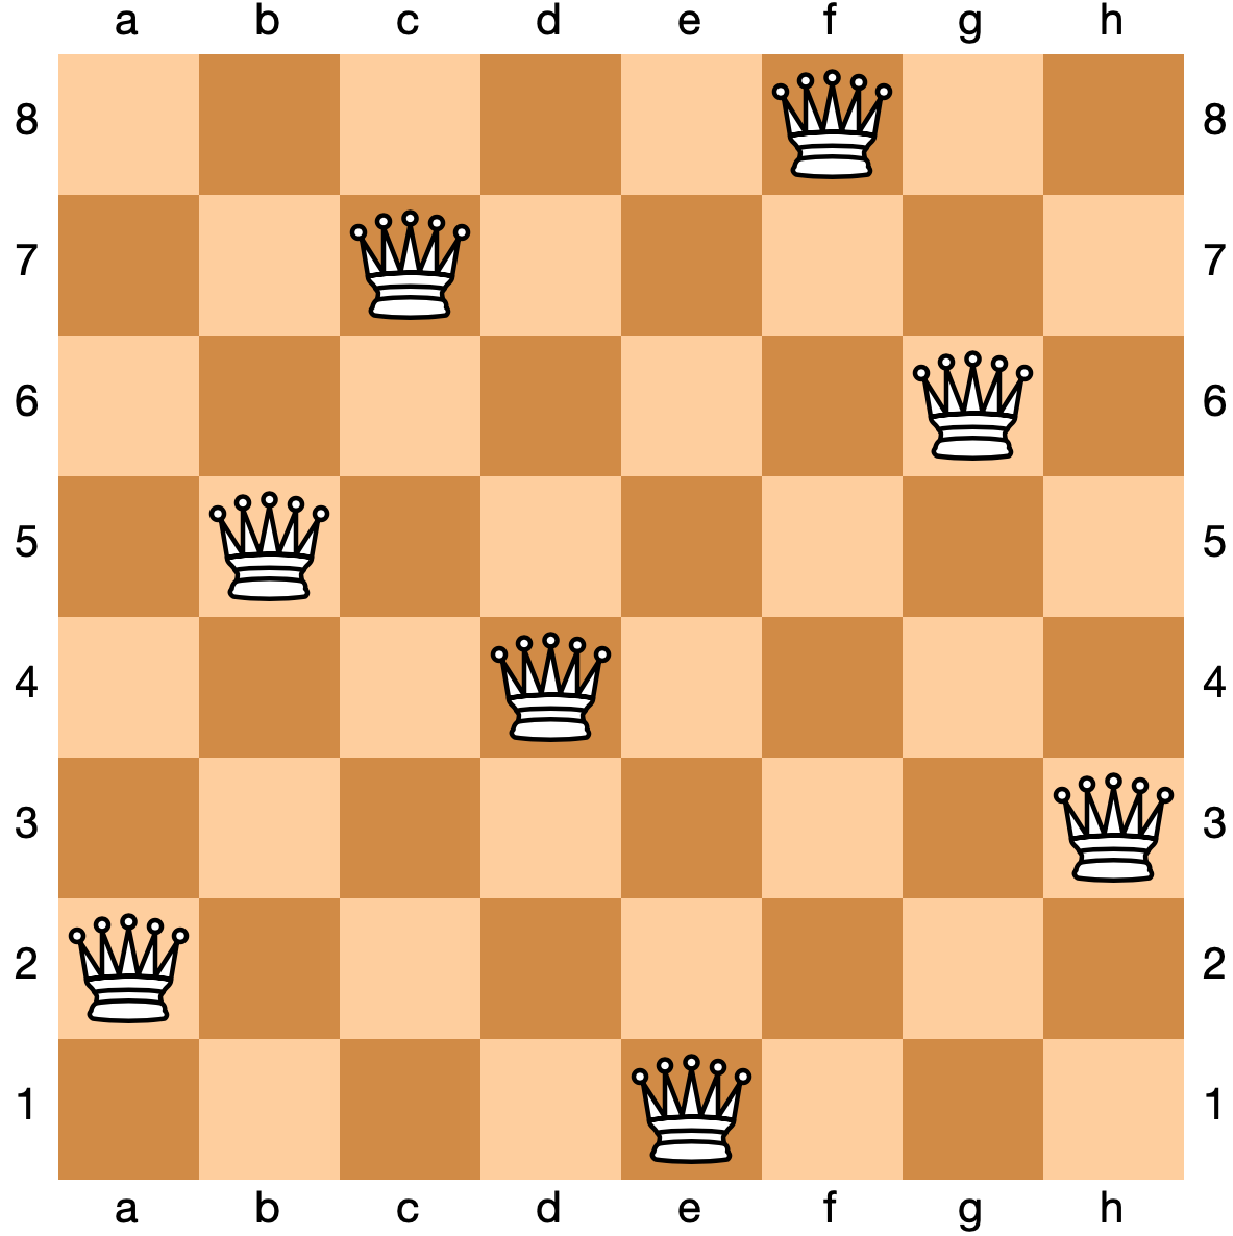
\epsfig{file=Figures/8-queens.pdf, scale=0.8}} 
  \caption{Eine Lösung des 8-Damen-Problems.}
  \label{fig:8-queens.pdf}
\end{figure}

Jessica Roth und Koen Loogman (das sind zwei ehemalige DHBW-Studenten) haben eine Animation des Verfahren von
Davis und Putnam implementiert.  Sie können diese Animation unter der Adresse
\\[0.2cm]
\hspace*{1.3cm}
\href{https://koenloogman.github.io/Animation-Of-N-Queens-Problem-In-JavaScript/}{https://koenloogman.github.io/Animation-Of-N-Queens-Problem-In-JavaScript/}
\\[0.2cm]
im Netz finden und ausprobieren.

Das 8-Damen-Problem ist natürlich nur eine spielerische Anwendung der Aussagen-Logik.
Trotzdem zeigt es die Leistungsfähigkeit des Algorithmus von Davis
und Putnam sehr gut, denn die Menge der Klauseln, die von der Funktion \texttt{allClauses}
berechnet wird, besteht aus 512 verschiedenen Klauseln.  In dieser Klausel-Menge kommen 64 verschiedene
Variablen vor. 

In der Praxis gibt es viele Probleme, die sich in ganz ähnlicher Weise auf die Lösung einer
Menge von Klauseln zurückführen lassen.  Dazu gehört zum Beispiel das Problem, einen
Stundenplan zu erstellen, der gewissen Nebenbedingungen genügt.  Verallgemeinerungen des
Stundenplan-Problems werden in der Literatur als \blue{Scheduling-Probleme} bezeichnet.
Die effiziente Lösung solcher Probleme ist Gegenstand der aktuellen Forschung.

\section{Reflexion}
\begin{enumerate}[(a)]
\item Wie haben wir die Menge der aussagenlogischen Formeln definiert?
\item Wie ist die Semantik der aussagenlogischen Formeln festgelegt worden?
\item Wie können wir aussagenlogische Formeln in \textsl{Python} darstellen?
\item Was ist eine Tautologie?
\item Was ist eine konjunktive Normalform?
\item Wie können Sie die konjunktive Normalform einer gegebenen aussagenlogischen Formel berechnen und wie lässt
      sich diese Berechnung in \textsl{Python} implementieren?
\item Wie haben wir den Beweis-Begriff $M \vdash C$ definiert?
\item Welche Eigenschaften hat der Beweis-Begriff $\vdash$?
\item Wann ist eine Menge von Klauseln lösbar?
\item Wie funktioniert das Verfahren von Davis und Putnam?
\item Wie können Sie das 8-Damen-Problem als aussagenlogisches Problem formulieren?
\end{enumerate}

%\section{Der Kompaktheits-Satz der Aussagen-Logik}
Das Ziel dieses Abschnittes ist der Beweis des Kompaktheits-Satzes der Aussagen-Logik.  
Dieser Satz liegt tiefer als alle bisher behandelten S\"{a}tze.  Wir ben\"{o}tigen den Kompaktheits-Satz
sp\"{a}ter, um die Widerlegungs-Vollst\"{a}ndigkeit der Pr\"{a}dikaten-Logik beweisen zu k\"{o}nnen.
Wir folgen bei unserer Darstellung des Kompaktheits-Satzes dem Artikel von Jon Barwise
\cite{barwise:1991a} aus dem Handbuch der mathematischen Logik \cite{barwise:1991}.

\begin{Definition}[endlich erf\"{u}llbar, maximal endlich erf\"{u}llbar]
  {\em Eine Menge $M$ von aussagenlogischen Formeln hei\3t \emph{endlich erf\"{u}llbar} (abgek\"{u}rzt: e.e.) genau
    dann, wenn jede endliche Teilmenge von $M$ erf\"{u}llbar ist:
    \\[0.2cm]
    \hspace*{1.3cm} 
    $M$ e.e. \quad g.d.w. \quad 
    $\forall E \subseteq M: \textsl{card}(E) < \infty \rightarrow 
    \exists \mathcal{I} \in \textsc{Ali}: \forall f \in E: \mathcal{I}(f) = \mathtt{true}$
    \\[0.2cm]
    Eine Menge $M$ von aussagenlogischen Formeln hei\3t \emph{maximal endlich erf\"{u}llbar}
    (abgek\"{u}rzt m.e.e.) genau dann, wenn $M$ endlich erf\"{u}llbar ist und wenn au\3erdem f\"{u}r
    jede aussagenlogische Formel $f$ entweder $f$ oder die Negation $\neg f$ ein Element von $M$ ist:
    \\[0.2cm]
    \hspace*{1.3cm}
    $M$ m.e.e. \quad g.d.w. \quad 
    $M$ e.e.$\;$ und $\;\forall f \el \mathcal{F}: f \el M \,\vee\, (\neg f) \el M$. \qed
  }
\end{Definition}

\begin{Satz} \label{satz28}
{\em
  Es sei $M$ maximal endlich erf\"{u}llbar.  Dann gilt 
  \\[0.2cm]
  \hspace*{1.3cm}
  $(f \wedge g) \el M$ \quad g.d.w. \quad $f \el M$ und $g \el M$.
}
\end{Satz}

\noindent
\textbf{Beweis}: Wir beweisen beide Richtungen des ``g.d.w.'' getrennt.
\begin{description}
\item[``$\Rightarrow$''] Sei $(f \wedge g) \el M$.  Wir f\"{u}hren den Beweis indirekt und
  nehmen an, es gelte $f \notel M$. Da
  $M$ maximal endlich erf\"{u}llbar ist, muss dann die Formel $\neg f$ ein Element der Menge
  $M$ sein.  Damit enth\"{a}lt $M$ aber die endliche Teilmenge 
  \\[0.2cm]
  \hspace*{1.3cm}
  $E := \{ f \wedge g, \neg f\}$, 
  \\[0.2cm]
  die offenbar nicht erf\"{u}llbar ist, denn jede Belegung, die $f \wedge g$ wahr macht, macht
  sicher auch $f$ wahr und damit $\neg f$ falsch.  Die Unerf\"{u}llbarkeit von $E$ steht im
  Widerspruch zur endlichen Erf\"{u}llbarkeit von $M$.  Damit muss die Annahme $f \notel M$
  falsch sein und wir haben $f \el M$ gezeigt. 

  Der Nachweis von $g \el M$ kann analog gef\"{u}hrt werden.
\item[``$\Leftarrow$''] Sei nun $f \el M$ und $g \el M$.  
  Wir f\"{u}hren den Beweis indirekt und nehmen an, dass $(f \wedge g) \notel M$ gelte.  Da $M$
  maximal endlich erf\"{u}llbar ist, muss dann die Formel $\neg (f \wedge g)$ ein Element der
  Menge $M$ sein.  Dann enth\"{a}lt $M$ aber die endliche Teilmenge
  \\[0.2cm]
  \hspace*{1.3cm}
  $E := \{ \neg (f \wedge g), f, g \}$
  \\[0.2cm]
  die offensichtlich nicht erf\"{u}llbar ist, denn jede Belegung, die $f$ und $g$ wahr macht,
  macht auch die Formel $f \wedge g$ wahr und muss damit die Formel $\neg (f \wedge g)$
  falsch machen.  Die Unerf\"{u}llbarkeit von $E$ steht im Widerspruch zur endlichen
  Erf\"{u}llbarkeit von $M$.  Damit muss die Annahme $(f \wedge g) \notel M$ falsch sein und
  es gilt $(f \wedge g) \el M$. \qed
\end{description}

\begin{Satz} \label{satz29}
{\em
  Es sei $M$ maximal endlich erf\"{u}llbar. Dann gilt:
  \begin{enumerate}
  \item $(\neg f) \el M$ \quad g.d.w. $f \notel M$.
  \item $(f \vee g) \el M$ \quad g.d.w. $f \el M$ oder $g \el M$.
  \item $(f \rightarrow g) \el M$ \quad g.d.w. $(\neg f) \el M$ oder $g \el M$.
  \item $(f \leftrightarrow g) \el M$ \quad g.d.w. 
        $(f \rightarrow g) \el M$ und $(g \rightarrow f) \el M$.
  \end{enumerate}
}
\end{Satz}

\noindent
\textbf{Beweis}:  Der Beweis der einzelnen Behauptungen verl\"{a}uft ganz analog zu dem Beweis
von Satz \ref{satz28}.  Exemplarisch zeigen wir den Beweis der vierten Behauptung.
Wir beweisen beide  Richtungen des ``g.d.w.'' getrennt.
\begin{description}
\item[``$\Rightarrow$''] Sei $(f \leftrightarrow g) \el M$.  Wir f\"{u}hren den Beweis indirekt und
  nehmen an, es gelte $(f \rightarrow g) \notel M$. Da
  $M$ maximal endlich erf\"{u}llbar ist, muss dann die Formel $\neg (f \rightarrow g)$ ein Element der Menge
  $M$ sein.  Damit enth\"{a}lt $M$ aber die endliche Teilmenge 
  \\[0.2cm]
  \hspace*{1.3cm}
  $E := \{ f \leftrightarrow g, \neg (f \rightarrow g)\}$, 
  \\[0.2cm]
  die offenbar nicht erf\"{u}llbar ist, denn jede Belegung, die $f \leftrightarrow g$ wahr macht, macht
  sicher auch $f \rightarrow g$ wahr und damit $\neg (f \rightarrow g)$ falsch.  Die
  Unerf\"{u}llbarkeit von $E$ steht im 
  Widerspruch zur endlichen Erf\"{u}llbarkeit von $M$.  Damit muss die Annahme $(f \rightarrow g) \notel M$
  falsch sein und wir haben $(f \rightarrow g) \el M$ gezeigt. 

  Der Nachweis von $(g \rightarrow f) \el M$ kann analog gef\"{u}hrt werden.
\item[``$\Leftarrow$''] Sei nun $(f \rightarrow g) \el M$ und $(g \rightarrow f) \el M$.  
  Wir f\"{u}hren den Beweis indirekt und nehmen an, dass $(f \leftrightarrow g) \notel M$ gelte.  Da $M$
  maximal endlich erf\"{u}llbar ist, muss dann die Formel $\neg (f \leftrightarrow g)$ ein Element der
  Menge $M$ sein.  Dann enth\"{a}lt $M$ aber die endliche Teilmenge
  \\[0.2cm]
  \hspace*{1.3cm}
  $E := \{ \neg (f \leftrightarrow g), f \rightarrow g, g \rightarrow f \}$
  \\[0.2cm]
  die offensichtlich nicht erf\"{u}llbar ist, denn jede Belegung, die $f \rightarrow g$ und $g
  \rightarrow f$ wahr macht,
  macht auch die Formel $f \leftrightarrow g$ wahr und muss damit die Formel $\neg (f \leftrightarrow g)$
  falsch machen.  Die Unerf\"{u}llbarkeit von $E$ steht im Widerspruch zur endlichen
  Erf\"{u}llbarkeit von $M$.  Damit muss die Annahme $(f \leftrightarrow g) \notel M$ falsch sein und
  es gilt $(f \leftrightarrow g) \el M$. \qed
\end{description}

\begin{Satz} \label{satz30}
{\em
  Jede maximal endlich erf\"{u}llbare Menge $M$ ist erf\"{u}llbar.
}
\end{Satz}

\noindent
\textbf{Beweis}:
Die Menge $M$ sei maximal endlich erf\"{u}llbar.  Wir konstruieren eine Variablen-Belegung
$\mathcal{I}$ wie folgt:
\\[0.2cm]
\hspace*{1.3cm}
$\mathcal{I} := \bigl\{ \pair(p, \mathtt{true})  \mid p \el M \bigr\} \cup
                \bigl\{ \pair(p, \mathtt{false}) \mid p \notel M \bigr\}$.
\\[0.2cm]
Wir behaupten, dass diese Belegung  jede Formel $f\el M$ wahr und jede Formel $f \notel M$
falsch macht und beweisen diese
Behauptung durch Induktion nach dem Aufbau der Formel $f$. Wir beweisen also
\\[-0.2cm]
\hspace*{1.3cm}
$f \el M$ \quad g.d.w. \quad $\mathcal{I}(f) = \mathtt{true}$
\\[0.2cm]
durch Induktion nach $f$.
\begin{enumerate}
\item $f = p \el \mathcal{P}$, \ $f$ ist also eine aussagenlogische Variable.
    
      Falls $p \el M$ ist, dann folgt $\mathcal{I}(f) = \mathtt{true}$ aus der Definition
      von $\mathcal{I}$.   Falls $p \notel M$ ist, folgt aus der Definition von
      $\mathcal{I}$ sofort $\mathcal{I}(p) = \mathtt{false}$.
      
\item $f = \neg g$.  

      Sei zun\"{a}chst $f \el M$. Nach Satz \ref{satz29} folgt aus $(\neg g) \el M$ sofort
      $g \notel M$.  Nach Induktions-Voraussetzung gilt dann $\textsl{I}(g) = \mathtt{false}$ und
      daraus folgt sofort $\textsl{I}(f) = \textsl{I}(\neg g) = \mathtt{true}$.
      
      Sei nun $f \notel M$. Wieder nach Satz \ref{satz29} folgt aus $(\neg g) \notel M$ sofort
      $g \el M$.  Nach Induktions-Voraussetzung gilt dann $\textsl{I}(g) = \mathtt{true}$ und
      daraus folgt sofort $\textsl{I}(f) = \textsl{I}(\neg g) = \mathtt{false}$.
\item $f = (g \wedge h)$.

      Sei zun\"{a}chst $f \el M$.  Nach Satz \ref{satz29} folgt aus $(g \wedge h) \el M$ sofort
      $g \el M$ und $h \el M$.  Wenden wir die Induktions-Voraussetzung auf $g$ und $h$ an, so sehen
      wir, dass $\textsl{I}(g) = \mathtt{true}$ und
      $\textsl{I}(h) = \mathtt{true}$ gelten muss, woraus sofort
      $\textsl{I}(f) = \textsl{I}(g \wedge h) = \mathtt{true}$ folgt.
      
      Sei nun $f \notel M$. Nach Satz \ref{satz29} folgt aus $(g \wedge h) \notel M$, dass
      entweder $g \notel M$ oder $h \notel M$ ist.  Wir betrachten nur den Fall $g \notel M$, 
      der Fall $h \notel M$ ist analog.  Aus $g \notel M$ folgt mit der Induktions-Voraussetzung,
      dass $\mathcal{I}(g) = \mathtt{false}$ gilt.  Dass impliziert aber die Behauptung 
      $\textsl{I}(g \wedge h) = \mathtt{false}$, womit wir $\mathcal{I}(f) = \mathtt{false}$ haben.
\item $f = (g \vee h)$,
      $f = (g \rightarrow h)$,
      $f = (g \leftrightarrow h)$.
      
      Da der Beweis dieser F\"{a}lle ganz analog zum Beweis des Falles $f = (f \wedge g)$ verl\"{a}uft,
      k\"{o}nnen wir auf einen expliziten Beweis dieser F\"{a}lle verzichten. \qed
\end{enumerate}

\begin{Satz}[Kompaktheits-Satz]
{\em
  Die Menge $M$ sei endlich erf\"{u}llbar.  Dann ist $M$ erf\"{u}llbar, es gibt also eine aussagenlogische
  Belegung $\mathcal{I}$, so dass gilt:
  \\[0.2cm]
  \hspace*{1.3cm}
  $\forall f \in M: \mathcal{I}(f) = \mathtt{true}$.
} 
\end{Satz}

\noindent
\textbf{Beweis}:  Wir werden $M$ so zu einer maximal endlich erf\"{u}llbaren Menge $\widehat{M}$
erweitern, dass 
\\[0.2cm]
\hspace*{1.3cm}
$M \subseteq \widehat{M}$
\\[0.2cm]
gilt.  Da die Menge $\widehat{M}$ nach Satz \ref{satz30} erf\"{u}llbar ist, ist $M$ als Teilmenge von
$\widehat{M}$ dann erst recht erf\"{u}llbar.
Zu diesem Zweck definieren wir eine Folge $(M_n)_{n\in \mathbb{N}}$ von Mengen, die alle endlich
erf\"{u}llbar sind und die in einem gewissen Sinne gegen die Menge $\widehat{M}$ konvergieren.
Die Definition der Mengen $M_n$ verl\"{a}uft durch Induktion nach der Zahl $n$.  Bevor wir diese
Induktion durchf\"{u}hren k\"{o}nnen, ben\"{o}tigen wir eine \emph{Aufz\"{a}hlung} aller aussagenlogischen Formeln.
Darunter verstehen wir eine Folge aussagenlogischer Formeln $(g_n)_{n \in \mathbb{N}}$, in der jede
aussagenlogische Formel mindestens einmal vorkommt, es soll also gelten:
\\[0.2cm]
\hspace*{1.3cm}
$\forall f \in \mathcal{F}: \exists n \in \mathbb{N}: f = g_n$.
\\[0.2cm]
Falls die Menge der Aussagen-Variablen endlich ist, so kann eine solche Folge zum Beispiel dadurch konstruiert
werden, dass wir erst alle Formeln der L\"{a}nge 1, dann die Formeln der L\"{a}nge 2 und so weiter
aufz\"{a}hlen.  

Die induktive Definition der Mengen $M_n$ verl\"{a}uft nun wie folgt.
\begin{enumerate}
\item[I.A.] $n = 0$:  Wir setzen
  \\[0.2cm]
  \hspace*{1.3cm}
  $M_0 := M$.
  \\[0.2cm]
  Dann ist die Menge $M_0$ nach Voraussetzung endlich erf\"{u}llbar.
\item[I.S.] $n \mapsto n + 1$:  Die Definition von $M_{n+1}$ erfolgt \"{u}ber eine Fall-Unterscheidung:
  \\[0.2cm]
  \hspace*{1.3cm}
  $M_{n+1} := \left\{
  \begin{array}[c]{ll}
    M_n \cup \{ f_n \}      & \mbox{falls $M_n \cup \{ f_n \}$ endlich erf\"{u}llbar ist;} \\[0.2cm]
    M_n \cup \{ \neg f_n \} & \mbox{sonst.}
  \end{array}
  \right.
  $
  \\[0.2cm]
  Wir m\"{u}ssen zeigen, dass $M_{n+1}$ endlich erf\"{u}llbar ist.  Es gibt zwei F\"{a}lle.
  \begin{enumerate}
  \item $M_n \cup \{ f_n \}$ ist endlich erf\"{u}llbar.

        Dann gilt $M_{n+1} = M_n \cup \{ f_n \}$ und die Behauptung ist trivial.
  \item $M_n \cup \{ f_n \}$ ist nicht endlich erf\"{u}llbar.

        Da $M_n$ alleine nach Induktions-Voraussetzung endlich erf\"{u}llbar ist, muss es dann eine
        endliche Teilmenge $E = \{ e_1, \cdots, e_k \} \subseteq M_n$ geben, so dass
        \\[0.2cm]
        \hspace*{1.3cm}
        $E \cup \{ f_n \}$
        \\[0.2cm]
        nicht erf\"{u}llbar ist.  Damit gilt dann
        \\[0.2cm]
        \hspace*{1.3cm}
        $\{ e_1, \cdots, e_m, f_n \} \models \falsum$
        \\[0.2cm]
        und daraus folgt
        \\[0.2cm]
        \hspace*{1.3cm}
        $ \models e_1 \wedge \cdots \wedge e_n \rightarrow \neg f_n$.
        \\[0.2cm]
        Wir f\"{u}hren den Beweis nun indirekt und nehmen an, dass die Menge
        \\[0.2cm]
        \hspace*{1.3cm}
        $M_n \cup \{ \neg f_n \}$ 
        \\[0.2cm]
        nicht endlich erf\"{u}llbar w\"{a}re.  Dann gibt es eine endliche Menge 
        $G = \{ g_1, \cdots, g_k \} \subseteq M_n$,
        so dass gilt:
        \\[0.2cm]
        \hspace*{1.3cm}
        $\{ g_1, \cdots, g_k, \neg f_n \} \models \falsum$.
        \\[0.2cm]
        Daraus folgt aber
        \\[0.2cm]
        \hspace*{1.3cm}
        $\models g_1 \wedge \cdots \wedge g_k \rightarrow f_n$.
        \\[0.2cm]
        Insgesamt haben wir damit aber sowohl
        \\[0.2cm]
        \hspace*{1.3cm}
        $\models e_1 \wedge \cdots \wedge e_m \wedge g_1 \wedge \cdots \wedge g_k \rightarrow f_n$
        \\
        als auch 
        \\[-0.2cm]
        \hspace*{1.3cm}
        $\models e_1 \wedge \cdots \wedge e_m \wedge g_1 \wedge \cdots \wedge g_k \rightarrow \neg f_n$.
        \\[0.2cm]
        Zusammengenommen zeigt dies, dass die Menge $G := \{ e_1, \cdots, e_m, g_1, \cdots, g_k \}$
        nicht erf\"{u}llbar ist:
        \\[0.2cm]
        \hspace*{1.3cm}
        $\{ e_1, \cdots, e_m, g_1, \cdots, g_k \} \models \falsum$.
        \\[0.2cm]
        Dies steht im Widerspruch dazu, dass diese Menge eine endliche Teilmenge von $M_n$ ist und
        $M_n$ ist nach Induktions-Voraussetzung endlich erf\"{u}llbar.  Daher haben wir die Annahme,
        dass $M_n \cup \{ \neg f_n \}$ nicht endlich erf\"{u}llbar ist, widerlegt. 
  \end{enumerate}
  Nach Konstruktion der Mengen $M_n$ gilt offenbar
  \\[0.2cm]
  \hspace*{1.3cm}
  $M_0 \subseteq M_1 \subseteq M_2 \subseteq \cdots \subseteq M_n \subseteq M_{n+1} \subseteq \cdots$.
  \\[0.2cm]
  Daher definieren wir die Menge $\widehat{M}$ nun als den Grenzwert der Folge $(M_n)_{n \in \mathbb{N}}$:
  \\[0.2cm]
  \hspace*{1.3cm}
  $\widehat{M} = \bigcup\limits_{n \in \mathbb{N}} M_n$.
  \\[0.2cm]
  Wir zeigen zun\"{a}chst, dass $\widehat{M}$ endlich erf\"{u}llbar ist.  Sei also $E$ eine endliche
  Teilmenge von $\widehat{M}$:
  \\[0.2cm]
  \hspace*{1.3cm}
  $E = \{ e_1, \cdots, e_m \} \subseteq \bigcup\limits_{n \in \mathbb{N}} M_n$.
  \\[0.2cm]
  Dann gibt es f\"{u}r jedes $i \in \{ 1, \cdots, m \}$ eine Zahl $n(i)$, so dass
  \\[0.2cm]
  \hspace*{1.3cm}
  $e_i \in M_{n(i)}$ 
  \\[0.2cm]
  ist.  Wir definieren
  \\[0.2cm]
  \hspace*{1.3cm}
  $\widehat{n} := \max\bigl(\bigl\{n(1), \cdots, n(m) \bigr\}\bigr)$
  \\[0.2cm]
  Daraus folgt aber sofort $E \subseteq M_{\widehat{n}}$ und da $M_{\widehat{n}}$ endlich erf\"{u}llbar
  ist, muss die Menge $E$ als endliche Teilmenge von $M_{\widehat{n}}$ erf\"{u}llbar sein.
  Damit haben wir gezeigt, dass $\widehat{M}$ endlich erf\"{u}llbar ist.

  Als n\"{a}chstes zeigen wir, dass $\widehat{M}$ maximal endlich erf\"{u}llbar ist.  Betrachten wir eine
  beliebige aussagenlogische Formel $f$.  Wir m\"{u}ssen zeigen, dass entweder $f \el \widehat{M}$ oder 
  $(\neg f) \el \widehat{M}$ gilt.  Wir hatten vorausgesetzt, dass die Folge $(f_n)_{n \in \mathbb{N}}$ 
  die Menge aller aussagenlogischen Formeln aufz\"{a}hlt.  Also gibt es ein $n$, so dass $f = f_n$ ist.
  Nach Definition gilt dann aber 
  \\[0.2cm]
  \hspace*{1.3cm}
  $M_{n+1} = M_n \cup \{ f_n \}$ \quad oder \quad 
  $M_{n+1} = M_n \cup \{ \neg f_n \}$
  \\[0.2cm]
  und da $M_{n+1} \subseteq \widehat{M}$ ist, folgt
  \\[0.2cm]
  \hspace*{1.3cm}
  $f_n \el \widehat{M}$ \quad oder \quad
  $(\neg f_n) \el \widehat{M}$.
  \\[0.2cm]
  Also ist $\widehat{M}$ maximal endlich erf\"{u}llbar und daher ist $\widehat{M}$ nach Satz \ref{satz30} erf\"{u}llbar. \qed
\end{enumerate}

%%% Local Variables: 
%%% mode: latex
%%% TeX-master: "logik"
%%% End: 


%%% Local Variables: 
%%% mode: latex
%%% TeX-master: "logic"
%%% ispell-local-dictionary: "deutsch8"
%%% End: 
